%==============================================================================
%  OpenRC - Open Region Computation Library
%  Codebase guide
%
%  Build:  latexmk -pdf openrc_guide.tex
%==============================================================================
\documentclass[11pt,a4paper]{report}

\usepackage[utf8]{inputenc}
\usepackage[T1]{fontenc}
\usepackage{lmodern}
\usepackage[margin=2.6cm]{geometry}
\usepackage{amsmath,amssymb}
\usepackage{booktabs}
\usepackage{longtable}
\usepackage{array}
\usepackage{enumitem}
\usepackage{xcolor}
\usepackage{graphicx}
\usepackage{listings}
\usepackage{upquote}
\usepackage{caption}
\usepackage{subcaption}
\usepackage{tikz}
\usetikzlibrary{arrows.meta,positioning,fit,backgrounds,calc,shapes.geometric}
\usepackage[most]{tcolorbox}
\usepackage{titlesec}
\usepackage{fancyhdr}
% Long module paths in \texttt must be breakable, or they run
% into the margin.
\usepackage[htt]{hyphenat}
\usepackage[colorlinks=true,linkcolor=nbblue,urlcolor=nbblue,citecolor=nbblue]{hyperref}
\hypersetup{pdftitle={OpenRC: User and Method Guide},pdfauthor={eesgong}}

%------------------------------------------------------------------ colours ---
\definecolor{nbblue}{HTML}{2E6DA4}
\definecolor{nbgrey}{HTML}{555555}
\definecolor{codebg}{HTML}{F6F8FA}
\definecolor{coderule}{HTML}{D0D7DE}
\definecolor{keyword}{HTML}{0550AE}
\definecolor{strcol}{HTML}{0A7D33}
\definecolor{comcol}{HTML}{6E7781}
\definecolor{warnbg}{HTML}{FFF6E5}
\definecolor{warnrule}{HTML}{D9822B}
\definecolor{notebg}{HTML}{EDF4FB}

%------------------------------------------------------------------ listings --
\lstdefinestyle{py}{
  language=Python,
  basicstyle=\ttfamily\footnotesize,
  keywordstyle=\color{keyword}\bfseries,
  stringstyle=\color{strcol},
  commentstyle=\color{comcol}\itshape,
  showstringspaces=false,
  backgroundcolor=\color{codebg},
  frame=single,
  rulecolor=\color{coderule},
  framesep=5pt,
  xleftmargin=6pt,
  breaklines=true,
  columns=fullflexible,
  keepspaces=true,
  morekeywords={with,as,yield,None,True,False,self}
}
\lstdefinestyle{sh}{
  language={},
  keywords={},
  basicstyle=\ttfamily\footnotesize,
  backgroundcolor=\color{codebg},
  frame=single,
  rulecolor=\color{coderule},
  framesep=5pt,
  xleftmargin=6pt,
  breaklines=true,
  columns=fullflexible,
  keepspaces=true
}
\lstset{style=py,upquote=true}

%-------------------------------------------------------------------- boxes ---
\newtcolorbox{notebox}[1][]{
  enhanced, breakable, sharp corners,
  colback=notebg, colframe=nbblue, boxrule=0.4pt,
  left=7pt, right=7pt, top=6pt, bottom=6pt,
  borderline west={2.5pt}{0pt}{nbblue}, #1}

\newtcolorbox{warnbox}[1][]{
  enhanced, breakable, sharp corners,
  colback=warnbg, colframe=warnrule, boxrule=0.4pt,
  left=7pt, right=7pt, top=6pt, bottom=6pt,
  borderline west={2.5pt}{0pt}{warnrule}, #1}

\newcommand{\why}[1]{\par\medskip\begingroup\noindent #1\par\endgroup\medskip}
\newcommand{\trap}[1]{\begin{warnbox}#1\end{warnbox}}

%--------------------------------------------------------------- shorthands ---
\newcommand{\code}[1]{\texttt{\small #1}}
\newcommand{\pymod}[1]{\texttt{\small\color{nbblue} #1}}
\newcommand{\file}[1]{\texttt{\small\color{nbgrey} #1}}

%------------------------------------------------------------------ headers ---
\pagestyle{fancy}
\fancyhf{}
\fancyhead[L]{\small\color{nbgrey}\leftmark}
\fancyhead[R]{\small\color{nbgrey}\thepage}
\renewcommand{\headrulewidth}{0.3pt}

\titleformat{\chapter}[display]
  {\normalfont\huge\bfseries\color{nbblue}}{\chaptertitlename\ \thechapter}{16pt}{\Huge}
\titlespacing*{\chapter}{0pt}{-20pt}{26pt}

\setlist[itemize]{leftmargin=1.4em,itemsep=0.25em,topsep=0.4em}
\setlist[enumerate]{leftmargin=1.6em,itemsep=0.25em,topsep=0.4em}
\setlist[description]{leftmargin=1.4em,itemsep=0.35em,topsep=0.4em,style=nextline}
\captionsetup{font=small,labelfont={bf,color=nbblue}}
% Let TeX loosen a line rather than push an unbreakable \code{...} word
% into the margin.
\setlength{\emergencystretch}{2.5em}

% Shared styles for the schematics.
\tikzset{
  blk/.style={draw=nbblue, fill=notebg, rounded corners=2pt, align=center,
              inner sep=4pt, font=\scriptsize},
  res/.style={draw=nbgrey, fill=codebg, rounded corners=2pt, align=center,
              inner sep=3pt, font=\scriptsize},
  lab/.style={font=\scriptsize, color=nbgrey},
  arr/.style={-{Stealth[length=4pt]}, draw=nbgrey},
  axis/.style={-{Stealth[length=4pt]}, draw=nbgrey},
  vtx/.style={circle, fill=nbblue, inner sep=1.2pt},
}

%==============================================================================
\begin{document}

\hypersetup{pageanchor=false}
\begin{titlepage}
\centering
\vspace*{2.5cm}
{\Huge\bfseries\color{nbblue} OpenRC\par}
\vspace{0.6em}
{\LARGE Open Region Computation Library\par}
\vspace{2.2em}
{\Large User and Method Guide\par}
\vspace{1.2em}
{\large Security regions for radial distribution networks\par}
\vfill
\begin{minipage}{0.82\textwidth}
\small
OpenRC computes polyhedral approximations of feasible power exchanges at
selected points of connection. This guide describes the network conventions,
power-flow models, construction methods, validation procedures and Python API.

\medskip
The source studies and their implementations are listed in
Chapter~\ref{ch:provenance}. Reproduced numerical results are reported in
Chapter~\ref{ch:evidence}.
\end{minipage}
\vfill
{\normalsize Version 0.1.0 \quad\textperiodcentered\quad MIT License,
 \copyright\ 2026 eesgong\par}
\vspace{1cm}
\end{titlepage}
\hypersetup{pageanchor=true}

\tableofcontents

%==============================================================================
\chapter*{Getting started}
\addcontentsline{toc}{chapter}{Getting started}
\markboth{Getting started}{}

\textbf{Installation.} In the source directory containing
\file{pyproject.toml}, run:

\begin{lstlisting}[style=sh]
python -m pip install .
python -c "import OpenRC; print(OpenRC.__version__)"
# Optional plotting, memory tools and Gurobi bindings:
python -m pip install '.[viz,resources,gurobi]'
\end{lstlisting}

The runtime requires Python 3.9 or newer; the optional development tools require
Python 3.11 or newer. For an editable checkout use
\code{python -m pip install -e .}; installing \file{requirements.txt} alone
installs dependencies, not OpenRC. Solver bindings need an appropriate licence.
The installed package carries its network data and works outside the source
directory; tutorials, scripts and this guide are supplied in the source
distribution. Project-specific verification and generated outputs should be
kept separately from the release tree.

\medskip
\noindent
\textbf{Tutorial.} Chapters~\ref{ch:idea} and~\ref{ch:architecture} introduce
the region representation and software structure. The executable tutorial
covers the main workflow:

\begin{lstlisting}[style=sh]
python examples/tutorial.py --list
python examples/tutorial.py      # quick start, with the equation-candidate example
python examples/tutorial.py 14   # run only that example
\end{lstlisting}

\noindent
\textbf{Conventions.} Chapter~\ref{ch:conventions} defines units, signs and
axis labels. These conventions apply to all public interfaces.

\medskip
\noindent
\textbf{Network import.} Chapter~\ref{ch:pandapower} covers
\code{pandapowerNet} import and the built-in network catalogue. The conversion
report records modelling choices and identifies applicable oracle families.

\medskip
\noindent
\textbf{Construction and certification.} Chapter~\ref{ch:conservative}
describes the conservative constructions. Section~\ref{sec:certificate}
separates global operating-limit bounds from solution existence and states the
assumptions of each certificate scope.

\medskip
\noindent
\textbf{Reference.} Chapter~\ref{ch:recipes} collects common workflows,
Chapter~\ref{ch:cli} covers the command line, and
Appendix~\ref{app:api} is the API summary.

%==============================================================================
\chapter{Security-region computation}
\label{ch:idea}

\section{The security region}

A security region describes the feasible active and reactive power exchanges
at selected points of connection (POCs). Each coordinate corresponds to a bus
quantity, so three selected quantities define a three-dimensional region.
Related terms include \emph{hosting capacity region}, \emph{feasible
operating region} and \emph{dynamic operating envelope}. OpenRC represents
these sets by convex polytopes.

The polytope $\{x : Ax \le b\}$ replaces power-flow constraints in downstream
optimisation. When the objective and remaining constraints are linear, this
gives an LP over the selected POC variables. Its validity depends on the network model and on the region's
approximation and validation scope.

\begin{center}
\resizebox{\textwidth}{!}{%
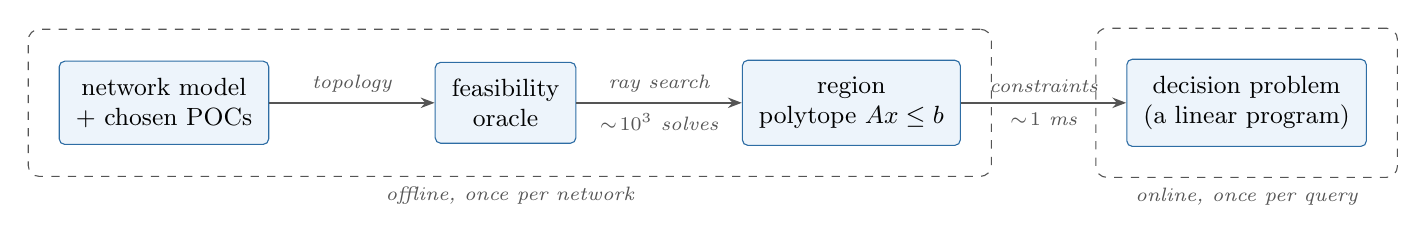
\begin{tikzpicture}[
  box/.style={draw=nbblue, fill=notebg, rounded corners=2pt, align=center,
              inner sep=6pt, font=\small},
  lab/.style={font=\scriptsize\itshape, color=nbgrey},
  ar/.style={-{Stealth[length=5pt]}, thick, draw=nbgrey}]

\node[box] (net) {network model\\+ chosen POCs};
\node[box, right=2.1cm of net] (or) {feasibility\\oracle};
\node[box, right=2.1cm of or] (reg) {region\\polytope $Ax\le b$};
\node[box, right=2.1cm of reg] (app) {decision problem\\(a linear program)};

\draw[ar] (net) -- node[lab, above]{topology} (or);
\draw[ar] (or) -- node[lab, above]{ray search}
                   node[lab, below]{$\sim\!10^3$ solves} (reg);
\draw[ar] (reg) -- node[lab, above]{constraints}
                   node[lab, below]{$\sim\!1$ ms} (app);

\begin{scope}[on background layer]
  \node[fit=(net)(reg), draw=nbgrey, dashed, rounded corners,
        inner sep=11pt, label={[lab]below:offline, once per network}] {};
  \node[fit=(app), draw=nbgrey, dashed, rounded corners,
        inner sep=11pt, label={[lab]below:online, once per query}] {};
\end{scope}
\end{tikzpicture}}
\end{center}

\section{The offline/online split}

Region construction typically requires hundreds to thousands of power-flow
queries. Once computed for a fixed network model, operating limits and base
point, the same region can serve repeated connection requests, preference-weight
sweeps, Pareto-front calculations or capacity-allocation problems.

\why{Construction and compression are evaluated mainly by oracle calls,
geometry cost and memory use. Applications are evaluated by solution time and
objective value. The software interfaces separate these stages.}

\section{Region representation}

A region is stored as a \textbf{vertex set}, and its convex hull is the region.
Two derived forms are computed on demand and cached (a region \emph{built} from
inequalities keeps them exactly, Section~\ref{sec:setops}):

\begin{description}
\item[The hull] gives the facets and the hypervolume. Hypervolume is the
  geometric coverage measure, reported alongside feasibility validation.
\item[The half-space form $Ax \le b$] is how membership is tested and how the
  region enters an optimisation model, with one row per stored inequality.
\end{description}

Facet count can dominate geometry cost: one measured 8-D region with
60 vertices had over 28\,000 facets. Chapters~\ref{ch:execution}
and~\ref{ch:compression} describe memory control and compression.

%==============================================================================
\chapter{Software architecture}
\label{ch:architecture}

\section{The layers}

\begin{center}
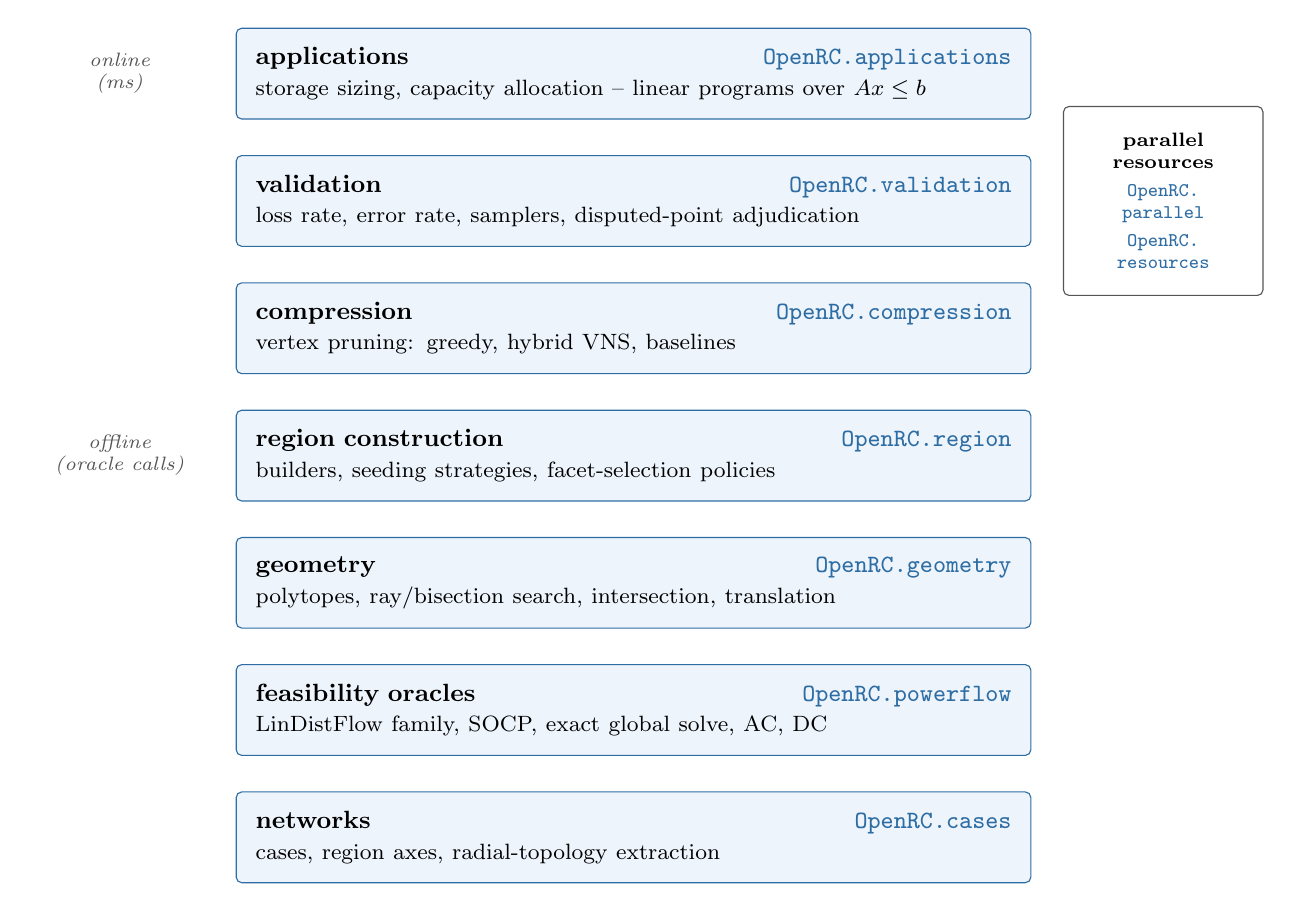
\begin{tikzpicture}[
  layer/.style={draw=nbblue, fill=notebg, rounded corners=2pt, align=left,
                text width=9.6cm, inner sep=7pt, font=\small},
  side/.style={font=\scriptsize\itshape, color=nbgrey, align=center,
               text width=2.1cm},
  node distance=4.5mm]

\node[layer] (app) {\textbf{applications} \hfill \pymod{OpenRC.applications}\\
  \footnotesize storage sizing, capacity allocation -- linear programs over $Ax\le b$};
\node[layer, below=of app] (val) {\textbf{validation} \hfill \pymod{OpenRC.validation}\\
  \footnotesize loss rate, error rate, samplers, disputed-point adjudication};
\node[layer, below=of val] (comp) {\textbf{compression} \hfill \pymod{OpenRC.compression}\\
  \footnotesize vertex pruning: greedy, hybrid VNS, baselines};
\node[layer, below=of comp] (reg) {\textbf{region construction} \hfill \pymod{OpenRC.region}\\
  \footnotesize builders, seeding strategies, facet-selection policies};
\node[layer, below=of reg] (geo) {\textbf{geometry} \hfill \pymod{OpenRC.geometry}\\
  \footnotesize polytopes, ray/bisection search, intersection, translation};
\node[layer, below=of geo] (pf) {\textbf{feasibility oracles} \hfill \pymod{OpenRC.powerflow}\\
  \footnotesize LinDistFlow family, SOCP, exact global solve, AC, DC};
\node[layer, below=of pf] (cas) {\textbf{networks} \hfill \pymod{OpenRC.cases}\\
  \footnotesize cases, region axes, radial-topology extraction};

\node[side, left=3mm of app] {online\\(ms)};
\node[side, left=3mm of reg] {offline\\(oracle calls)};

\node[draw=nbgrey, fill=white, rounded corners=2pt, right=4mm of val,
      text width=2.3cm, align=center, font=\scriptsize, minimum height=2.4cm]
      (par) {\textbf{parallel}\\\textbf{resources}\\[2pt]
             {\ttfamily\color{nbblue} OpenRC.\\parallel}\\[2pt]
             {\ttfamily\color{nbblue} OpenRC.\\resources}};
\end{tikzpicture}
\end{center}

Region algorithms query a feasibility-oracle interface rather than embedding
power-flow equations. The same construction method can therefore use a linear,
conic or AC model, subject to the model's assumptions and verdict semantics.

\section{Component registries}

Sixteen component families use a \code{Registry}. Implementations are added
with a registration decorator:

\begin{lstlisting}
from OpenRC.compression.base import COMPRESSORS, Compressor

@COMPRESSORS.register("my-method", doc="One line, shown in --help")
class MyCompressor(Compressor):
    name = "my-method"
    def _run(self, polytope, *, target_vertices, max_volume_loss_pct):
        ...
\end{lstlisting}

Registration makes the compressor available through
\code{get\_compressor("my-method")}, the component listing, CLI and benchmark
interfaces.

\begin{table}[h]
\centering\small
\caption{The sixteen registries}
\begin{tabular}{@{}llp{6.4cm}@{}}
\toprule
Registry & Module & Scope \\
\midrule
\code{CASES}           & \pymod{cases.builtin}        & Network models and axis presets \\
\code{ORACLES}         & \pymod{powerflow.base}       & Power-flow feasibility oracles \\
\code{EQUATION\_SOLVERS} & \pymod{powerflow.equations} & Local equation candidates, independently verified \\
\code{STRUCTURED\_SOLVERS} & \pymod{powerflow.equations} & Network-structured solver candidates, such as the certified sweep (Section~\ref{sec:sweep}) \\
\code{MODELING\_LAYERS} & \pymod{powerflow.modeling} & Solver modelling backends (Section~\ref{sec:modeling}) \\
\code{BUILDERS}        & \pymod{region.base}          & Region construction methods \\
\code{SEEDS}           & \pymod{region.base}          & Initial polytope seeding strategies \\
\code{FACET\_POLICIES} & \pymod{region.facet\_policy} & Facet-selection policies \\
\code{FACET\_SCREENS}  & \pymod{region.facet\_policy} & Candidate-facet pre-filters \\
\code{COMPRESSORS}     & \pymod{compression.base}     & Vertex-pruning methods \\
\code{SCHEDULES}       & \pymod{compression.schedule} & Online compression triggers and targets \\
\code{REFINERS}        & \pymod{region.refine}        & Fixed-cardinality vertex refinement \\
\code{RAY\_STRATEGIES} & \pymod{region.ray\_growth}   & Ray-direction and vertex-update strategies \\
\code{SAMPLERS}        & \pymod{validation.samplers}  & Validation sampling distributions \\
\code{APPLICATIONS}    & \pymod{applications.base}    & Downstream optimisation problems \\
\code{BENCHMARK\_METHODS} & \pymod{benchmark}          & Methods compared by the benchmark harness \\
\bottomrule
\end{tabular}
\end{table}

\code{orc.registries()} lists the implementations available in the installation.

\why{Worker processes reconstruct cases and oracles from registered names and
factory options. This avoids transferring live solver handles between
processes (Section~\ref{sec:workers}).}

\clearpage
\section{Source layout}

\begin{lstlisting}[style=sh,basicstyle=\ttfamily\scriptsize]
OpenRC/
  OpenRC/                    the package
    registry.py              the Registry class
    utils.py                 logging, timing
    resources.py             memory budgets, hull-size measurement
    parallel.py              worker pools, sequential/parallel planning
    benchmark.py             random instances, paired runs, intervals
    cases/                   networks + region axes
      pandapower_adapter.py  any pandapowerNet -> GridCase
      pp_networks.py         pandapower.networks, registered lazily as pp:<name>
      data/<name>/*.csv      curated network tables
    powerflow/               feasibility oracles; modeling.py: Pyomo,
                             MOSEK or Gurobi modelling layers;
                             equations.py: SciPy/custom candidate interface;
                             sweep.py: certified radial fixed-point sweeps;
                             interval.py: outward-rounded interval arithmetic
    geometry/                polytopes, ray search, set operations,
                             live_hull.py: the hull kept alive while growing
    region/                  builders, seeds, facet policies and screens,
                             refine.py: vertex relocation at a fixed size,
                             ray_growth.py: pluggable ray strategies
    compression/             vertex pruning; schedule.py: when to compress
    validation/              loss/error rate, samplers, adjudication,
                             inner-region certificate, existence proof,
                             verification modes
    applications/            decision problems
    viz.py                   plots (optional; imports matplotlib lazily)
  scripts/
    demo.py                  command-line driver
    benchmark.py             methods x networks x dimensions x seeds
    benchmark_memory.py      growth under a memory budget, by schedule
    benchmark_performance.py timings across networks, with intervals
    generate_readme_figures.py
                             regenerates the README figures
  examples/
    tutorial.py              the runnable tutorial
  docs/                      this document; the README figures
\end{lstlisting}

%==============================================================================
\chapter{Units and conventions}
\label{ch:conventions}

The conventions below apply across the library. Earlier unit and indexing
inconsistencies are documented in Section~\ref{sec:unitbug}.

\section{Units}

\begin{center}
\begin{tabular}{@{}ll@{}}
\toprule
Quantity & Unit at every public interface \\
\midrule
Active power & MW (three-phase) \\
Reactive power & Mvar (three-phase) \\
Voltage & kV (line-to-line) \\
Current & kA \\
\bottomrule
\end{tabular}
\end{center}

The DistFlow models are written in SI per-phase units (W, V, A, $\Omega$).
Unit conversion is performed in \pymod{powerflow/distflow.py} via
\code{scale = 1e6 / 3.0}.

\section{Sign}

\textbf{Positive is consumption.} A region coordinate is the \emph{additional}
power a POC may draw, so a negative coordinate means generation or export. The
origin of region space is the network's base operating point.

\section{Axes}

A region dimension is a \code{(bus, quantity)} pair, where quantity is
\code{"p"} or \code{"q"}. The first four calls below produce the same axes
on the 9-bus case; the last defines a mixed P/Q region:

\begin{lstlisting}
case.resolve_axes("247")            # a named preset
case.resolve_axes([1, 3, 6])        # bus indices
case.resolve_axes("1,3,6")          # a comma string (the CLI form)
case.resolve_axes(["1p","3p","6p"]) # fully explicit
case.resolve_axes(["1p","1q"])      # a mixed P/Q region at one bus
\end{lstlisting}

\trap{Bus indices are \textbf{0-based}, while preset \emph{names} follow the
1-based numbering of the papers. ``POC 2,4,7'' is the preset \code{"247"}, which
resolves to buses \code{[1, 3, 6]}.}

\section{Determinism}

Builders accept \code{seed\_rng} for reproducible random streams. Reproduction
also requires the same model, numerical settings and software versions.
Parallel batch APIs return results in input order; serial and worker
comparisons are included in the validation workflow.

%==============================================================================
\chapter{Networks}
\label{ch:cases}

\section{\code{GridCase}}

\file{OpenRC/cases/base.py}

A \code{GridCase} contains the \code{pandapower} network, per-bus base
injections in MW/Mvar, nominal voltage, voltage limits and named axis presets.
It provides the network data used by the oracle and region interfaces.

\begin{lstlisting}
case = orc.get_case("9bus")
print(case.summary())

case.n_bus, case.n_line, case.slack_bus
case.base_p_mw            # per-bus, consumption positive
case.topology             # lazily built RadialTopology
case.resolve_axes("247")  # -> RegionAxes
case.injection_vector(axes, delta)   # -> full per-bus (p, q) arrays
\end{lstlisting}

\section{Included networks and primary test cases}

\begin{center}\small
\begin{tabular}{@{}>{\raggedright\arraybackslash}p{4.7cm}r>{\raggedright\arraybackslash}p{8.9cm}@{}}
\toprule
Case & Buses & Description and primary role \\
\midrule
\code{9bus} & 9 & Built-in Dutch 10.5\,kV radial MV feeder at nameplate ratings; 3-D to 16-D growth, conservative methods, certification and memory-budget tests \\
\code{9bus-scaled} & 9 & Built-in 9-bus variant (ratings $\times 6$, cable lengths $\div 3$); 8-D growth and vertex-compression studies \\
\code{cigre-hv} & 13 & Built-in 380\,kV CIGRE HV benchmark with transformers (meshed; \code{dcopf}, \code{acopf}) \\
\code{pp:case33bw} & 33 & IEEE 33-bus Baran--Wu 12.66\,kV radial feeder; cross-network 3/5/8-D benchmarks, interval sweep and unrated-branch handling \\
\code{pp:mv\_oberrhein} (\code{feeder=1}) & 109 & Radial substation area of pandapower's 20\,kV MV Oberrhein network; large-feeder growth, worker scaling and 3/5/8-D benchmarks \\
\code{pp:create\_cigre\_network\_mv} (\code{load\_scale=0.8}) & 15 & 20\,kV CIGRE MV feeder (two collapsed transformers, three open ties); transformer collapse, line charging and 3/5/8-D benchmarks \\
\code{pp:case9} & 9 & WSCC 345\,kV transmission ring (meshed; radiality guard and \code{dcopf} tests) \\
\code{pp:<name>} & -- & Any of the 60 networks in \code{pandapower.networks}; oracle applicability is classified in Chapter~\ref{ch:pandapower} \\
\bottomrule
\end{tabular}
\end{center}

\noindent The 9-bus feeder is described in S.~Gong, \emph{Grid Feasibility with
Massive Integration: A Dutch MV Charging Infrastructure Case}, PhD thesis,
Eindhoven University of Technology, 2025.

\subsection{Load scaling}
\label{sec:loadscale}

Region growth requires a feasible starting point. A network whose recorded
operating point violates its own limits therefore needs reduced loading or
another feasible origin. The \code{load\_scale} argument applies a common
scaling factor to loads and static generators and so selects a different
operating point. The \code{pp:mv\_oberrhein} feeder (\code{feeder=1}), for
example, is feasible as recorded: AC power flow gives a minimum voltage of
0.930\,p.u. and a maximum line loading of 86.2\,\%. At \code{load\_scale=1.5}
it is not (0.873\,p.u., 136.6\,\%). Variants are cached separately:

\begin{lstlisting}
orc.get_case("9bus", load_scale=0.70)
orc.get_case("pp:mv_oberrhein", feeder=1, load_scale=0.70)
\end{lstlisting}

\paragraph{Configuration lifetime.} Oracles, point verifiers and adjudicators
use private configuration snapshots. Use \code{rebuild} to derive a variant:
\begin{lstlisting}
case = orc.get_case("pp:mv_oberrhein", feeder=1)
lighter = case.rebuild(load_scale=0.4)
oracle = orc.get_oracle("lindistflow", lighter)
\end{lstlisting}
\code{rebuild} clears derived caches and rescales the recorded injections,
including recovery from zero load. To change network tables, edit a private
copy and re-import it with \code{case\_from\_pandapower}; the edited tables
then define the new base. Configuration checks run at task boundaries and
exclude solver results and internal working state. Custom workflows can use
\code{case.assert\_unchanged()} and \code{case.snapshot()}. Cases must remain
unchanged during a computation or snapshot operation. Extension copy hooks
retain responsibility for their own state; implementation details are in the
README.

\trap{\code{9bus} and \code{9bus-scaled} are not interchangeable. Under the
scaled ratings the \code{tight-intersect} construction cannot start at the
default origin, because its worst-case loss/voltage correction
grows with the \emph{square} of the current rating. Section~\ref{sec:method2}
has the details.}

\section{Radiality and root selection}
\label{sec:radiality}

\file{OpenRC/powerflow/topology.py}

\subsection{DistFlow applicability}

DistFlow applicability is checked before root selection. A graph is a tree
when it has one connected component and $E = V - 1$; the number of independent
loops is the cyclomatic number $E - V + C$.

The DistFlow family requires one connected component, no loops, supported
electrical elements and at most one infeed. Multiple infeeds may occur in
separate components or in a connected network. Component extraction is
described in Chapter~\ref{ch:pandapower}, using \code{mv\_oberrhein}
(two infeeds) and \code{lv\_schutterwald} (fourteen) as examples.

\begin{lstlisting}
case.is_radial                 # bool
case.radiality                 # RadialityReport
print(case.radiality.message)  # one actionable paragraph
\end{lstlisting}

The native AC/DC power-flow and OPF oracles support meshed networks
(Section~\ref{sec:opf}). A failed DistFlow applicability check therefore
restricts the choice of oracle rather than excluding the network from OpenRC.

DistFlow reports unsupported topology or devices before constructing a tree or
solver model. The diagnostic lists the reasons and alternative oracle families:

\begin{lstlisting}[style=sh]
MeshedNetworkError: case 'cigre-hv': the DistFlow oracles cannot be used on
this network because it contains 6 two-winding transformers, which the
DistFlow oracles cannot represent directly (on a radial network,
OpenRC.case_from_pandapower collapses two-winding transformers into equivalent
branches automatically); it is MESHED: 13 buses and 15 branches leave 3
independent loop(s), where a radial network has exactly 12 branches and none
(open the loops to a radial configuration). This restricts the DistFlow family
only - the network still has a security region. Compute it with an oracle that
carries no radiality assumption: 'dcopf'/'acopf' if the generation is
dispatchable, or 'dcpf'/'acpf' to evaluate a fixed dispatch.
\end{lstlisting}

\trap{Radiality checks include
\code{net.line}, \code{net.trafo}, \code{net.impedance} and
\code{net.trafo3w} (with \code{trafo3w} represented as a star from its HV
winding) and exclude out-of-service rows. The 13-bus CIGRE
network has 15 branches and three loops when transformers are included; its
six transformers also require a model outside the direct DistFlow formulation.}

\code{MeshedNetworkError} and \code{AmbiguousSlackError} both subclass
\code{ValueError}, so a handler for \code{ValueError} catches them.

\subsection{Automatic root selection}

A radial feeder's upstream connection defines the tree root. OpenRC infers
this bus from the network and records the selection rule:

\begin{lstlisting}
case.slack_bus      # 8
case.slack_source   # 'external grid'
\end{lstlisting}

The selection rules are applied in this order:

\begin{enumerate}
\item a single external grid;
\item a single slack generator;
\item the unique bus at the highest nominal voltage, which on a distribution
  feeder is the substation busbar;
\item if several buses share that voltage, the unique one among them with a
  single incident branch, corresponding to the feeder head.
\end{enumerate}

If these rules do not identify a unique bus, OpenRC raises
\code{AmbiguousSlackError}. For example, a path at one voltage with no
declared infeed has two indistinguishable ends.

\begin{lstlisting}
# only when the network itself does not identify its infeed
GridCase(..., slack_bus_override=3)   # slack_source == 'explicit slack_bus_override'
\end{lstlisting}

\why{The recorded \code{slack\_source} makes the root selection auditable.
An incorrect root changes branch orientation and power-flow results even if
the graph remains a valid tree.}

\subsection{The tree}

Once the root is known, \code{RadialTopology} derives the parent/child structure
by breadth-first search, giving each branch its parent, child, $r$, $x$ and
thermal limit, plus the mapping from bus index to variable position.

\why{Topology extraction replaces the network-specific root and variable
indices used in the original scripts (Section~\ref{sec:unitbug}).}

The queries \code{path\_to\_root(bus)}, \code{depth(bus)} and
\code{electrical\_distance(bus)} describe each POC's position relative to the
substation and help interpret differences in voltage sensitivity.

\section{Adding a network}

Use \code{case\_from\_pandapower} for existing network models
(Chapter~\ref{ch:pandapower}). The CSV format below is intended for curated
cases distributed with the library.

Place four files in \file{OpenRC/cases/data/<name>/}:

\begin{center}\small
\begin{tabular}{@{}ll@{}}
\toprule
\file{bus.csv}  & \code{bus, name, vn\_kv, vm\_min\_pu, vm\_max\_pu, is\_slack} \\
\file{line.csv} & \code{line, name, from\_bus, to\_bus, length\_km, r\_ohm\_per\_km,} \\
                & \code{x\_ohm\_per\_km, c\_nf\_per\_km, max\_i\_ka, std\_type} \\
\file{load.csv} & \code{bus, name, p\_mw, q\_mvar} (several rows per bus are summed) \\
\file{meta.json}& \code{v\_nom\_kv}, \code{poc\_presets}, \code{notes} \\
\bottomrule
\end{tabular}
\end{center}

Register the case in \file{OpenRC/cases/builtin.py}:

\begin{lstlisting}
_register_tabular_case("my-feeder", DATA_ROOT / "my-feeder",
                       doc="One line describing the network.")
\end{lstlisting}

(The IEEE 33-bus Baran--Wu feeder does not need this: it is already available
as \code{pp:case33bw}.)

Branch parameters are stored per line rather than through a standard-type
library, so each directory is self-contained and can be inspected or edited
directly as plain text.

A programmatically constructed case uses a zero-argument factory returning
\code{GridCase}; \code{cigre-hv} provides an example.

%==============================================================================
\chapter{Pandapower network import}
\label{ch:pandapower}

\file{OpenRC/cases/pandapower\_adapter.py} \quad
\file{OpenRC/cases/pp\_networks.py}

The adapter imports \code{pandapowerNet} objects, JSON network files and
networks from \code{pandapower.networks}. The native AC/DC oracles retain
meshes, transformers and multiple infeeds. DistFlow applicability is checked
separately against its topology and device assumptions.

\begin{lstlisting}
import pandapower as pp
import OpenRC as orc

case = orc.case_from_pandapower(my_net, name="my-feeder",
                                axis_presets={"poc": [1001, 1045, 1102]})
case = orc.case_from_pandapower(pp.from_json("feeder.json"))
case = orc.get_case("pp:case33bw")        # any built-in network, by name
orc.list_pandapower_networks()            # all sixty
orc.classify_pandapower_networks()        # which oracles apply to each
orc.get_case("pp:create_cigre_network_mv",           # pandapower builder options
             network_kwargs={"with_der": "pv_wind"})  # (preserved across workers)
\end{lstlisting}

Built-in networks are constructed on first use and cached. Each
\code{get\_case} call returns a private copy. Keyword options are passed to
the adapter; for example, \code{orc.get\_case("pp:mv\_oberrhein", feeder=1)}
selects one AC component.

\section{Conversion and model assumptions}

The conversion report is stored in \code{case.metadata["conversion"]}.

\subsection{Switch states}

Switch states determine the operating topology. An open-ring MV feeder, for
example, can operate radially. The adapter applies switch states before
classifying connectivity:

\begin{center}\small
\begin{tabular}{@{}lll@{}}
\toprule
Switch & State & Effect \\
\midrule
line / transformer (\code{et="l"}, \code{"t"}) & open   & the switched terminal is disconnected \\
bus--bus (\code{et="b"}, $z=0$)                 & closed & the buses are fused \\
bus--bus (\code{et="b"}, $z>0$)                 & closed & the impedance is preserved \\
bus--bus (\code{et="b"})                        & open   & no connection \\
\bottomrule
\end{tabular}
\end{center}

One open terminal does not take an entire line out of service: the connected
end can still draw charging current. AC retains the native line and switch
model; a line with both ends disconnected is removed. The branch-flow
conducting graph excludes open-terminal branches. Its default
\code{line\_charging="omit"} omits their shunts as it does for closed lines;
\code{"constant"} explicitly rejects single-open capacitive lines, whose
terminal equivalent is not represented. Finite-impedance bus couplers also
remain available to AC/DC/OPF and are outside the DistFlow model.

\trap{Switch handling changes the classification of
\code{simple\_mv\_open\_ring\_net} from a structural ring to an operating
tree. It also preserves the connectivity of \code{example\_multivoltage},
whose buses are joined by closed bus--bus switches; omitting those switches
would create 32 apparent components.}

\subsection{Transformers: collapse through per-unit}

The branch-flow models use one nominal voltage. For networks with a substation
transformer, the adapter forms a series equivalent on a common reference base.
For a branch with per-unit impedance $z_{pu}$ on base $S_{base}$, the
equivalent at reference voltage $V_{ref}$ is
\[
  z = z_{pu} \frac{V_{ref}^2}{S_{base}}, \qquad
  I^{max} = \frac{s^{max}_{pu} \, S_{base}}{\sqrt{3} \, V_{ref}} .
\]
Applying this conversion to lines and transformers gives a single-voltage
series-equivalent network. The curated 9-bus cases use the same
idealisation for their substation transformer.

\code{transformer\_handling="auto"} (the default) collapses only when the network
is already a tree. Transformer collapse preserves connectivity and therefore
does not make a meshed network eligible for DistFlow.

\trap{The collapse accepts the standard series per-unit idealisation: an
off-nominal tap position, phase shift and no-load branch are not represented.
All are detected and listed in the conversion warnings. Conversion is atomic:
if any transformer lacks usable data, no unrepresented transformer is deleted.}

\subsection{Compatibility contract}

AC power flow checks voltage plus loading in \code{line}, \code{trafo} and
\code{trafo3w}; a transformer-only network is valid. For lines, DistFlow uses
$I^{max}=\code{max\_i\_ka}\,\code{df}\,\code{parallel}$ and divides series
impedance by \code{parallel}, matching pandapower. \code{load\_scale} scales
\code{load}, \code{sgen} and \code{storage} together. AC validation keeps each
bus's native voltage limits; the scalar DistFlow representation uses the
strictest common interval across non-infeed buses. If there is no common interval, AC/DC/OPF remain
available and DistFlow is disabled explicitly. When a case specifies a scalar
voltage envelope different from that derived from the bus table (for example,
via direct construction or \code{case.rebuild(vm\_min\_pu=...)}), the
overridden envelope is applied to every non-infeed bus in both AC and DistFlow,
whether stricter or looser; when the bus table has no common interval, the
envelope recorded at import serves as the reference. Kept transformers,
impedance branches, voltage-controlled generators, voltage-dependent shunts or ZIP loads,
Ward/xWard equivalents, motors, FACTS compensators and AC/DC converters are
rejected by the DistFlow family but stay
available to AC/DC/OPF. A generic OPF solver failure remains
\code{INCONCLUSIVE}. Parallel workers rebuild the full case
recipe, including dict-valued options and feeder/rating/transformer choices.

A disconnected bus with a nonzero requested total injection cannot be served,
even if pandapower converges after excluding that bus. AC checks both $P$ and
$Q$; the DC models check $P$ only because they have no reactive-power balance.
A zero total request remains admissible when a control injection cancels the
bus's base load.

Control loads offset the native fixed-power load, sgen and storage actually
present, including supported sgen limit clipping; separately declared case
bases still define the requested operating point. Native PV, shunt and ZIP
behaviour is retained. Thermal checks require full branch results even when
the source network requests voltage-only output.

\subsection{Asymmetric loads}

OpenRC uses single-phase equivalents of a balanced network. To keep AC, DC,
OPF and branch flow consistent across pandapower versions, each
\code{asymmetric\_load} or \code{asymmetric\_sgen} is replaced by an ordinary
element carrying its three-phase total. This includes the 907-bus IEEE
European LV feeder. A conversion warning records that phase imbalance is not
represented; upstream aggregation support depends on the version and solver.

\subsection{Placeholder ratings}
\label{sec:unrated}

MATPOWER-derived transmission cases often use placeholder thermal ratings.
MATPOWER encodes ``no limit'' as $\text{rateA} = 9900$\,MVA and pandapower
as $I^{max} = 99\,999$\,kA; the former becomes 41\,kA at 138\,kV and 27\,000\,kA
at 0.2\,kV, so the current alone does not reveal it. OpenRC therefore judges the
rating as apparent power, $\sqrt{3}\,V I$, and treats anything at or above
\textbf{9\,GVA} as unrated. For comparison, a 765\,kV circuit carries about
5\,GVA.

\begin{warnbox}
On \code{case33bw}, placeholder ratings caused models that bound branch losses
by $r \, I^{max\,2}$ to assign reactive losses of order $10^{11}$\,Mvar, and
caused the \code{socp} oracle to report the base point as \textbf{infeasible}
even though AC power flow converged, violating the outer-relaxation property.
Supplying a finite thermal rating resolved this discrepancy.
\end{warnbox}

In the branch-flow models, an unrated line has no thermal constraint;
\code{lindistflow}, \code{socp} and \code{exact} support this convention.
Native AC/DC/OPF oracles retain the ratings and loading limits in the imported
\code{pandapower} network, so a finite placeholder remains a finite constraint.
Model-II and both Method-2 models
use the thermal rating to bound neglected branch losses and therefore raise
\code{UnratedBranchError} when a branch is unrated. An explicit rating can be
supplied when appropriate for the study:

\begin{lstlisting}
orc.get_case("pp:case33bw", default_rating_ka=0.4)   # explicit thermal rating
\end{lstlisting}

\subsection{Bus numbering}

OpenRC uses contiguous zero-based bus indices. The adapter renumbers custom
IDs and gaps left by bus fusion, translates axis presets from the original
IDs, and records the map in the conversion metadata.

\begin{lstlisting}
case = orc.case_from_pandapower(net, axis_presets={"poc": [300, 400, 500]})
case.axis_presets["poc"]          # [2, 3, 4]
\end{lstlisting}

\subsection{Several feeders}

Separate AC components with their own infeeds can be selected individually.
Several infeeds alone do not imply independent or radial feeders. Extraction
preserves native devices and settings, and rejects cuts across HVDC/DC coupling
or remote AC controls that would change the physical problem:

\begin{lstlisting}
orc.list_feeders(pn.mv_oberrhein())       # feeder, infeed bus, size
case = orc.case_from_pandapower(pn.mv_oberrhein(), feeder=1)   # radial
\end{lstlisting}

\section{Built-in network catalogue}

\code{orc.classify\_pandapower\_networks()} builds and classifies every network.
With pandapower 3.4.0 and 3.5.6, all \textbf{60} networks import and
\textbf{27} are eligible for DistFlow
after switch handling and transformer collapse, and \textbf{33} require
AC/DC/OPF. Re-run after upgrading pandapower because its catalogue may change.

\begin{center}\small
\begin{tabular}{@{}lp{9.6cm}@{}}
\toprule
Radial -- DistFlow applies & \code{case33bw} (IEEE 33, Baran--Wu), the Kerber and
  \code{kb\_extrem} LV libraries, \code{ieee\_european\_lv\_asymmetric},
  \code{create\_synthetic\_voltage\_control\_lv\_network},
  \code{simple\_mv\_open\_ring\_net}, \code{create\_cigre\_network\_mv}, \dots \\[3pt]
AC/DC/OPF only & \code{case9} \dots\ \code{case9241pegase}, CIGRE HV,
  \code{example\_simple},
  \code{iceland}, \code{GBnetwork}, \code{example\_multivoltage}; and the
  multi-infeed \code{mv\_oberrhein}, \code{lv\_schutterwald},
  \code{case6495rte}. Inspect each extracted component: meshed or
  multi-infeed components still require the native models \\
\bottomrule
\end{tabular}
\end{center}

\trap{On \code{case33bw} with a 0.4\,kA
rating, \code{intersect-shift} with the default \code{shift\_scope="path"}
may fail to find a common shifted-slice centre. The accumulated worst-case
loss along the 17-branch path to bus 17 is a 4.4\,Mvar reactive shift.
An unsuccessful finite centre search is reported separately from an empty
polytope intersection and does not prove that the shifted slice is empty.
\code{shift\_scope="feeding\_branch"}
gives an 18-vertex region there, which the certificate proves inner. This region
excludes the base point: the remote feeder voltage requires some local
generation to accommodate the reactive-loss correction. Method~2 applies the
same per-branch loss bound and can encounter similar restrictions.}

\section{From the command line}

\code{-{}-case pp:<name>} and \code{-{}-case-file model.json} work with every
subcommand, together with \code{-{}-feeder}, \code{-{}-default-rating-ka},
\code{-{}-load-scale} and \code{-{}-transformer-handling}:

\begin{lstlisting}[style=sh]
python scripts/demo.py pp list
python scripts/demo.py pp classify --only case33bw,create_kerber_dorfnetz
python scripts/demo.py pp feeders --case mv_oberrhein
python scripts/demo.py region --case pp:case33bw --axes 17,24,32
python scripts/demo.py region --case-file my_feeder.json --axes 10,20,28
python scripts/demo.py region --case pp:mv_oberrhein --feeder 1 --axes 30,60,90
\end{lstlisting}


%==============================================================================
\chapter{Feasibility oracles}
\label{ch:oracles}

\section{Oracle interface and verdicts}

\file{OpenRC/powerflow/base.py}

An oracle assesses the feasibility of a per-bus injection vector. Region
algorithms use this common interface to query different power-flow models.

\begin{lstlisting}
oracle = orc.get_oracle("lindistflow", case)
oracle.feasible_at(axes, [1.0, 2.0, -0.5])   # -> bool
oracle.verdict_at(axes, [1.0, 2.0, -0.5])    # -> Verdict
oracle.stats.as_dict()                       # calls, time, ms/call
\end{lstlisting}

The answer is \textbf{three-valued}:

\begin{center}\small
\begin{tabular}{@{}lp{9.6cm}@{}}
\toprule
\code{Verdict.FEASIBLE} & An operating point exists and respects every limit. \\
\code{Verdict.INFEASIBLE} & No such operating point exists. \\
\code{Verdict.INCONCLUSIVE} & The solver could not decide. \\
\bottomrule
\end{tabular}
\end{center}

\why{Non-convergence of Newton--Raphson does not establish infeasibility.
\code{INCONCLUSIVE} preserves this distinction in validation results.
\code{bool(verdict)} is \code{True} only for \code{FEASIBLE}, so region
construction excludes points whose feasibility has not been established.}

Only an explicit solver termination \code{infeasible} is interpreted as an
infeasibility proof. Pyomo's \code{noSolution} means no feasible solution was
found; \code{infeasibleOrUnbounded} does not distinguish the two cases. Both
remain \code{INCONCLUSIVE}, as do direct exact-solver failures, with the latter
recorded in \code{last\_solve}. Candidate residuals must be finite and
non-negative in every constraint family; an undefined or overflowed cone
residual forces fallback.

\section{The LinDistFlow family}

\file{OpenRC/powerflow/distflow.py}

The exact branch-flow equations use per-phase SI quantities, with consumption
positive:
\begin{align}
P_{ij} &= \textstyle\sum_{k:(j,k)\in E} P_{jk} + r_{ij} l_{ij} + P_j
  \label{eq:bal} \\
Q_{ij} &= \textstyle\sum_{k:(j,k)\in E} Q_{jk} + x_{ij} l_{ij} + Q_j \\
v_j &= v_i - 2 (r_{ij} P_{ij} + x_{ij} Q_{ij}) + (r_{ij}^2 + x_{ij}^2) l_{ij}
  \label{eq:vdrop} \\
l_{ij} &= (P_{ij}^2 + Q_{ij}^2) / v_i \;\le\; l^{max}_{ij}
  \label{eq:therm}
\end{align}

Four convex models share one implementation. They differ in the loss term in
\eqref{eq:bal}, the treatment of $(r^2+x^2)l$ in \eqref{eq:vdrop}, and the use
of nameplate or tightened thermal limits in \eqref{eq:therm}.

\begin{table}[h]
\centering\small
\caption{The four production variants. The reproduction variants
\code{legacy-tight-voltage} and \code{legacy-tight-flow} are retained for
archive reproduction and are not used by \code{ConservativeBuilder}.}
\begin{tabular}{@{}llllp{3.1cm}@{}}
\toprule
Oracle & Balance loss & $v_{child}$ term & Thermal & Role \\
\midrule
\code{lindistflow}       & dropped & dropped            & nameplate & Method~1, Model~I \\
\code{lindistflow-vdrop} & dropped & $+(r^2{+}x^2)l^{max}$ & nameplate & Method~1, Model~II \\
\code{tight-voltage}     & dropped & $+(r^2{+}x^2)l^{max}$ & path-tightened & Method~2, Model~I \\
\code{tight-flow}        & $+r\,l^{max}$, $+x\,l^{max}$ & dropped & nameplate & Method~2, Model~II \\
\bottomrule
\end{tabular}
\end{table}

\subsection{Paired models}

The exact voltage carries $+(r^2+x^2)l$ with $l \in [0, l^{max}]$. A model that
sets $l = 0$ and one that sets $l = l^{max}$ therefore \textbf{bracket} the true
voltage, and their intersection is contained in the region of the model that
retains \eqref{eq:vdrop} exactly. Both methods use this bracket.

The methods treat the balance loss in \eqref{eq:bal} differently:

\begin{description}
\item[Method 1] leaves it out of both models and compensates afterwards, in
  region space, by requiring every combination of the $P$ and $Q$ loss shifts
  (Section~\ref{sec:method1}).
\item[Method 2] charges it inside \code{tight-flow}, and tightens
  \code{tight-voltage}'s thermal limits, so no translation is needed.
\end{description}

\subsection{Thermal tightening}

When a variant tightens, the limit becomes
$(I^{max} - \sqrt{\Delta l})^2$, where $\Delta l$ converts the loss power
accumulated along a branch's path into a current margin. The default scope is
the \textbf{complete path to the slack}. Two other scopes are available:
\code{"upstream\_legacy"} (the original scripts' scope, which omitted the
slack-connected branch) and \code{"subtree"}: the branch and everything below
it, whose losses are the ones that flow through it. With the subtree scope the
thermal check is taken at $v^{min}$, which makes Method~2 a theorem
(Section~\ref{sec:method2}).

\code{DistFlowOracle.binding\_tightening()} reports the tightened/nameplate
ratio per branch and can help diagnose an empty Method~2 component. On the
9-bus case the ratios range from 0.35 to 0.84, accounting for the volume
reduction in Table~\ref{tab:audit}.

\subsection{Closed-form evaluation}
\label{sec:closed-form}

For fixed injections, each variant has a unique solution obtained by tree
traversal: the balances determine branch flows, followed by voltage drops
from the slack. With $T$ the branch-by-bus subtree incidence ($T_{bj} = 1$ when
bus $j$ lies below branch $b$), the model reads
\begin{align*}
P &= T p + c_P, \qquad Q = T q + c_Q, \\
v &= v_0 \mathbf{1} - 2\,T^{\top}\!\left(r \circ P + x \circ Q\right) + c_v ,
\end{align*}
where the constants $c_P = T_{\cdot,\mathrm{child}}(r \circ l^{max})$,
$c_Q$ and $c_v = s\,T^{\top}((r^2{+}x^2)\circ l^{max})$ are the loss charges
selected by the variant's switches. Feasibility then reduces to the voltage
bounds and $P_b^2 + Q_b^2 \le l^{max,\mathrm{eff}}_b\, v_{\mathrm{parent}(b)}$,
each checked to a relative $10^{-9}$. \code{DistFlowOracle(backend="analytic")},
the default, evaluates these expressions using sparse $T$, with one entry per bus and branch
on its path to the slack, and \code{feasible\_mask} evaluates a whole batch
of points in one matrix product. \code{backend="solver"} keeps the Pyomo
model and a conic solver, as an independent cross-check. A subclass that
changes the model in \code{\_build} should either select it or override
\code{\_evaluate} to match.

\begin{center}\small
\begin{tabular}{@{}lrr@{}}
\toprule
 & 9-bus, 3-D & 9-bus, 8-D \\
\midrule
one query, analytic / solver     & 22\,\textmu s / 0.8\,ms & \\
per point in a batch of 2000     & 0.2\,\textmu s & \\
region build, analytic / solver  & 0.07 / 2.37\,s & 0.25 / 1.32\,s \\
\bottomrule
\end{tabular}
\end{center}

\noindent Region builds used \code{generation}, with 120 and 60 vertices.
Call counts were identical under both backends and volumes agreed to
$5\cdot10^{-5}$.

\paragraph{Agreement with the solver.} The two backends were compared on every
random point for all six variants on \code{9bus} (4-D), on \code{9bus-scaled}
(5-D) and on \code{pp:case33bw}. Every random point
received the same verdict. The observed disagreements occur within $3.2\cdot10^{-5}$
(relative) \emph{inside} the boundary. Within that band the solver rejects some
feasible points non-monotonically (for example, reporting ``infeasible'' at
$10^{-5}$ inside the boundary and ``feasible'' at $10^{-6}$ along the same ray),
whereas no exterior point was accepted. Regions produced with the analytic
backend are correspondingly slightly larger. The
archived 14-vertex volume (Chapter~\ref{ch:evidence}) is reproduced to
$+3.1\cdot10^{-5}$ instead of $\pm2\cdot10^{-5}$. A trajectory-sensitive
policy such as \code{adaptive-ema} amplifies such differences. Across five
bisection tolerances its 120-vertex Model-I volume averages
$542.6 \pm 6.2$ with the analytic backend and $542.5 \pm 10.4$ with the
solver. The regions are equally valid, but not bit-identical between backends.

\section{Reference and adjudicating oracles}

\begin{center}\small
\begin{tabular}{@{}llp{7.4cm}@{}}
\toprule
Oracle & Needs & Role \\
\midrule
\code{socp}  & MOSEK/Gurobi & Second-order-cone relaxation of the exact model.
  An \emph{outer} approximation. \\
\code{exact} & Gurobi \code{NonConvex=2} & Global solve of the exact equations.
  The adjudicator. \\
\code{acpf}  & \code{pandapower} & Newton--Raphson AC with limit checks; the
  first-line reference. \\
\code{dcpf}  & \code{pandapower} & DC flow, thermal limits only. Screening. \\
\code{dcopf} & \code{pandapower} & DC optimal power flow with dispatchable
  resources. No radiality requirement. \\
\code{acopf} & \code{pandapower} & AC optimal power flow. No radiality
  requirement. \\
\bottomrule
\end{tabular}
\end{center}

\subsection{Optimal power flow on meshed networks}
\label{sec:opf}

\file{OpenRC/powerflow/opf.py}

The DistFlow family checks a fixed injection pattern. The OPF oracles instead
optimise controllable generation to accommodate the requested injection,
subject to network and resource limits. They also support meshed networks.

\begin{lstlisting}
case = orc.get_case("cigre-hv")          # meshed, with transformers
region = ExpansiveBuilder().build(
    case, case.resolve_axes("026"),
    orc.get_oracle("dcopf", case), max_vertices=40).polytope
\end{lstlisting}

An OPF-ready network must specify power limits for controllable generators and
a cost on at least one resource. Missing data raises \code{NotOpfReadyError}.

The CIGRE-HV base point illustrates the distinction between fixed-dispatch
power flow and OPF:

\begin{center}\small
\begin{tabular}{@{}lll@{}}
\toprule
\code{dcpf}  & feasible     & fixed dispatch, thermal limits only \\
\code{acpf}  & infeasible   & fixed dispatch violates the voltage envelope \\
\code{dcopf} & feasible     & a dispatch exists \\
\code{acopf} & feasible     & a dispatch exists in the AC model \\
\bottomrule
\end{tabular}
\end{center}

\why{For both OPF oracles, a converged result proves feasibility. A generic
exception or non-convergence maps to \code{INCONCLUSIVE}: pandapower's wrapper
has not supplied a solver certificate that distinguishes true infeasibility
from a numerical or modelling failure.}

\trap{The interior-point AC-OPF is sensitive to its start. \code{acopf} tries a
power-flow solution, then a flat start (\code{inits=("pf", "flat")}), and calls a
point feasible once one converges. A flat start alone did not converge at the
CIGRE-HV base point, nor on 6 of 40 random points; both starts converged on 39
of 40, agreeing with \code{dcopf} on 39, in less time. \code{inits=("flat",)}
restores the single attempt. Screen with \code{dcopf} first where no start
converges.}

\paragraph{Reusing the AC model.} With \code{recycle=True} (default), a query
can reuse pandapower's internal model and the previous Newton--Raphson
solution. Reuse is restricted to previous feasible solutions. In one
\code{case33bw} test, starting from a heavily loaded state at 0.58\,p.u. led
the next query to a limit-violating low-voltage solution at 0.16\,p.u.; a flat
start found 0.94\,p.u. After an infeasible or inconclusive result, the next
query therefore starts flat. A recycled attempt that fails numerically or
converges outside a limit is also repeated from a flat start before the
remaining retry chain. Convergence of the recycled attempt alone does not
establish infeasibility.

Every ray search resets the warm state with \code{reset\_warm\_state}.
Without this reset, differences within Newton's tolerance changed subsequent
margin-search probes: boundary coordinates differed by $3\cdot10^{-14}$
according to the preceding rays, affecting bitwise agreement between serial
and parallel runs. With the reset, verdicts were identical on 680 random
points across four networks, in every order and region build compared.

The cross-network benchmark (Section~\ref{sec:performance}) found little
benefit from recycling alone: AC build times changed by factors of
0.95--1.05. For scattered queries, mean time decreased by 7\,\% on CIGRE MV
and increased by 7--17\,\% elsewhere; failed warm starts required an
additional flat solve. Recycling remains enabled with the confirmation rules
above. Most of the measured AC acceleration came from margin search.

pandapower's numba-compiled power flow is used whenever numba is installed
(\code{numba=None}): 1.8--1.9$\times$ per AC query with identical verdicts on
900 points, AC builds 1.8--2.6$\times$. Its voltages differ at $10^{-13}$,
which can redirect a trajectory; \code{numba=False} uses the uncompiled
power flow.

\trap{\textbf{Directional validity of relaxations and inner approximations.}
Because SOCP is an outer relaxation, an \emph{infeasible} verdict certifies
exact infeasibility, whereas a \emph{feasible} verdict leaves exact
feasibility undecided. Conversely, rejection by an inner approximation does
not establish exact infeasibility. The adjudicator applies these rules
according to each oracle's declared approximation role
(Section~\ref{sec:adjudication}).}

\why{The \code{exact} and \code{socp} oracles are formulated in a
\textbf{1\,MVA per-unit} base rather than SI. The SI form made Gurobi stop with
numerical difficulties on an ordinary $[2,2,2]$\,MW point; the algebraically
equivalent per-unit form returns \code{optimal} there and still proves
$[100,100,100]$\,MW infeasible. Through Pyomo, the SI form of \code{socp} left
Gurobi's barrier short of its tolerances at 17 of 18 feasible 9-bus points,
all reported inconclusive.}

\section{Pyomo and direct solver APIs}
\label{sec:modeling}

\file{OpenRC/powerflow/modeling.py}

Three oracles solve a model per query: \code{socp}, \code{exact}, and the
DistFlow family with \code{backend="solver"}. Only the injections change from
one query to the next, but Pyomo translates the whole model for the solver at
every solve. Each of these oracles therefore takes a \code{modeling} argument.

\begin{description}
\item[\code{"pyomo"} (default)] Pyomo formulation; \code{solver=} selects any
  compatible Pyomo solver. Serves as the portable reference implementation.
\item[\code{"mosek"}] MOSEK Fusion API. The model is constructed once with bus
  injections represented as a Fusion \code{Parameter} and reused across
  queries. Restricted to convex formulations (unsupported for \code{exact}).
\item[\code{"gurobi"}] Native \code{gurobipy} API. The model is constructed
  once and each query updates only the power-balance right-hand sides;
  supports the non-convex quadratic equality of \code{exact}.
\end{description}

The direct layers use a solver-neutral \code{ConicForm}, independently of the
Pyomo model:
$\min c^\top x$ subject to $Ax = b + Bu$ (with $u$ the per-bus injections),
$l \le x \le u_x$, and per branch $P_k^2 + Q_k^2 \le f_k g_k$ (or $=$ in the
exact model), where each factor is affine in a single variable.
\code{branch\_flow\_form} writes this form for all three oracles from the
network's SI constants. It divides them through by per-unit bases,
because in SI the coefficients span ten orders of magnitude. The SI form
caused Gurobi's barrier to stop short of optimality on feasible SOCP points,
which it then reported as infeasible. A new layer, such as CVXPY or another
solver interface, registers a class in \code{MODELING\_LAYERS}: it receives a
\code{ConicForm} and answers \code{verdict}.

\subsection{Optional equation candidates}
\label{sec:equation-candidate}

\file{OpenRC/powerflow/equations.py}

A Newton or Gauss--Seidel iteration finds a root; it does not prove that no root
exists. Nor does solving $Ax=b+Bu$ alone enforce the bounds and cones. OpenRC
therefore treats a fast local result as a \emph{candidate}, never as an
infeasibility certificate. The feature is opt-in through
\code{candidate\_solver="newton"} or \code{"gauss-seidel"}. The default is
\code{None}, so the configured optimiser remains the reference. A rejected
candidate always falls through to that optimiser.

\begin{figure}[h]
\centering
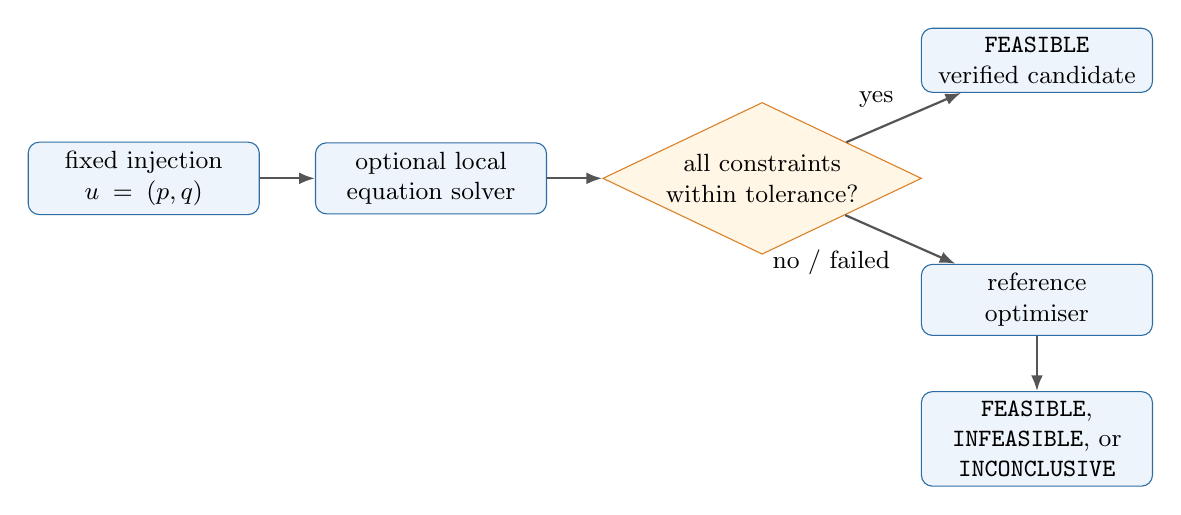
\begin{tikzpicture}[
  node distance=7mm and 7mm,
  every node/.style={font=\small},
  box/.style={draw=nbblue, rounded corners, fill=notebg, align=center,
              minimum height=8mm, text width=27mm},
  decision/.style={draw=warnrule, diamond, aspect=2.1, fill=warnbg,
                   align=center, inner sep=1.5pt},
  arrow/.style={-{Latex[length=2mm]}, thick, draw=nbgrey}
]
\node[box] (query) {fixed injection\\$u=(p,q)$};
\node[box, right=of query] (local) {optional local\\equation solver};
\node[decision, right=of local] (check) {all constraints\\within tolerance?};
\node[box, above right=6mm and 10mm of check] (yes) {\code{FEASIBLE}\\verified candidate};
\node[box, below right=6mm and 10mm of check] (opt) {reference\\optimiser};
\node[box, below=of opt] (verdict) {\code{FEASIBLE},\\\code{INFEASIBLE}, or\\\code{INCONCLUSIVE}};
\draw[arrow] (query) -- (local);
\draw[arrow] (local) -- (check);
\draw[arrow] (check) -- node[above left]{yes} (yes);
\draw[arrow] (check) -- node[below left]{no / failed} (opt);
\draw[arrow] (opt) -- (verdict);
\end{tikzpicture}
\caption{Candidate verification and optimiser fallback. Only the reference
optimiser may supply an infeasibility certificate.}
\label{fig:equation-fallback}
\end{figure}

Acceptance independently re-evaluates the scaled equality residual, lower and
upper bounds, non-negativity of both rotated-cone factors, and every cone
inequality. Pyomo exceptions and unknown termination conditions remain
\code{INCONCLUSIVE}; region construction treats that conservatively as outside,
while validation can escalate it.

\begin{lstlisting}
oracle = orc.get_oracle(
    "lindistflow", case,
    backend="solver",                 # optimiser remains the fallback
    modeling="mosek",
    candidate_solver="newton",       # or "gauss-seidel"
    candidate_tolerance=1e-9,
)
verdict = oracle.verdict_at(axes, point)
print(oracle.candidate_stats.as_dict())
print(oracle.describe()["last_candidate_certificate"])
\end{lstlisting}

Both inner-region constructions pass the same option to their component
models:

\begin{lstlisting}
builder = ConservativeBuilder(
    method="tight-intersect",
    oracle_kwargs={"backend": "solver",
                   "candidate_solver": "newton"})
\end{lstlisting}

The command-line equivalent is:

\begin{lstlisting}[style=sh]
python scripts/demo.py conservative --case 9bus --axes 247 \
  --oracle-option backend=solver \
  --oracle-option candidate_solver=newton
\end{lstlisting}

\why{The four linear DistFlow construction models have a square, nonsingular
affine equation matrix. Tree traversal evaluates their unique solution
directly (Section~\ref{sec:closed-form}), without Newton or Gauss--Seidel
iteration. Candidates are available with \code{backend="solver"} and can also
support extensions without a closed-form solution.}

The prepared Newton implementation caches one sparse LU factorisation and
changes only the right-hand side per query. Gauss--Seidel first obtains a
non-zero diagonal with a sparse bipartite matching, then caches the lower and
upper sparse factors. No candidate history is retained, so memory is linear in
the model size; the oracle's existing re-entrant lock protects the cache, and
each process worker builds its own. After preparation on this machine, full
candidate generation and checking took 0.036\,ms per Newton query on
9 buses and 0.71\,ms with Gauss--Seidel. The closed form remains about
0.02--0.03\,ms.

\subsection{Certified backward/forward sweeps}
\label{sec:sweep}

\file{OpenRC/powerflow/sweep.py}

\paragraph{Limitations of generic candidates.} On the SOCP and exact forms, the
exported equations are the linear ones only; the cones are checked
afterwards but are not equations. The system is under-determined, and a
Newton step can reach the affine set without satisfying a cone. From the default
start (the midpoint of the bounds, i.e.\ losses at half the rating) it also
diverged. A closed-form
LinDistFlow start converged in a few iterations, but the result was still rejected
at the cone boundary. Oracles therefore monitor candidate acceptance. After
\code{candidate\_patience} attempts (default 20), an acceptance rate below
\code{candidate\_min\_rate} (default 5\,\%) switches the candidate off; the
statistics record both \code{disabled} and the exact \code{disabled\_after}
attempt. Attempt counts must be positive integers.

\paragraph{Radial fixed-point iteration.} For the exact radial series-impedance
model with unit slack voltage (or slack voltage $v_0$ via
\code{slack\_vm\_pu}, replacing $\mathbf 1$ by $v_0\mathbf 1$ below), the bus
voltages satisfy $V = \mathbf 1 - Z\,\overline{s} \oslash \overline{V}$ with
$Z = T^{\top}\mathrm{diag}(z)\,T$. For two buses, $|V_2|^2$ is a root of a
quadratic. For larger feeders, OpenRC uses iterative sweeps rather than a
general closed-form solution. Each sweep is a closed-form \emph{step}: it
evaluates the right-hand side $F(V)$ as two sparse products, the currents
summed up the tree and the drops down it. Its first iterate, $V_1 = \mathbf 1 - Z\,\overline{s}$, is itself a
closed-form linear estimate. A converged iterate can be certified as follows.
For an iterate $\hat V$, let
$\delta = \|F(\hat V) - \hat V\|_\infty$. On the ball $B(\hat V, r)$ the map $F$ has
the Lipschitz bound
\[
  L(r) = \max_i \sum_j |Z_{ij}|\,|s_j| \,/\, (|\hat V_j| - r)^2
  \;\le\; \max_i \bigl[T^{\top}\bigl(|z| \circ T(|s| / (|\hat V| - r)^2)\bigr)\bigr]_i ,
\]
computed in $O(\mathrm{nnz}\,T)$. Require $0 < r < \min_j |\hat V_j|$,
$L(r) < 1$, and $\delta \le r\,(1 - L(r))$. The map then sends the closed
infinity-norm ball into itself as a contraction. By Banach's theorem it contains
a unique solution $V^\ast$ in $B(\hat V, r)$, with
$\|V^\ast - \hat V\|_\infty \le \delta/(1 - L(r))$ (uniqueness is local to the
ball rather than global). Every
voltage magnitude and every rated branch current is then checked against its
limit with that bound as margin; the bound on a current is
$\delta/(1-L)$ times the subtree sum of $|s_j|/((|\hat V_j| - r)|\hat V_j|)$. A
point that passes has a solution within all limits of the exact model, and
therefore of its SOC relaxation. The sweep does not claim infeasibility,
because a solution with large angles can lie outside the ball. The global
condition of Section~\ref{sec:certificate} (a ball around 1\,p.u., $\xi < 1/4$)
is more restrictive; this local one needs only $L < 1$
at the solution.

The full witness is public as
\code{RadialSweep.last\_certificate}: residual, ball radius, Lipschitz bound,
error bound, and the voltage/current margins after the enclosure.

\paragraph{Interval verification.} Evaluating these inequalities in floating
point does not prove them: every operation rounds, and a point whose margin is
smaller than the accumulated rounding error could be accepted wrongly. A safety
factor on the residual and the Lipschitz estimate alone is insufficient for a
proof. With \code{certificate="interval"} (the default), every point
that passes the floating-point test is therefore proven again in interval
arithmetic (\file{OpenRC/powerflow/interval.py}). IEEE~754 rounds $+$, $-$,
$\times$, $\div$ and $\sqrt{\ }$ correctly, so moving each computed bound one
ulp outward (\code{numpy.nextafter}) gives an interval that contains the exact
result; chaining such operations encloses every expression built from them.
The proof starts from the stored data ($r$, $x$, $s$, $\hat V$). It encloses
the per-unit impedances and the map $F(\hat V)$: the currents, then the subtree
and path sums, one outward-rounded addition at a time. From these it obtains
$\delta$, $L(r)$, $1 - L$, the error bound and the voltage and current margins,
each as the upper or lower bound the argument needs. The conditions then hold
for the real numbers, and the certificate's \code{rigorous} field is
\code{True}. \code{certificate="float"} keeps the floating-point test alone
(pass it with \code{candidate\_options=\{"certificate": "float"\}}).

The enclosures were checked against exact rational arithmetic
(\code{fractions.Fraction}) and 60-digit mpmath: 4\,000 elementary operations,
500 complex divisions and moduli, the tree sums of the \code{mv\_oberrhein} feeder, and
$F(\hat V)$, $\delta$ and $L$ at 24 points of two networks. All enclosures
contained the reference values. On the 720 points of the table below, the
proof accepted exactly the points the
floating-point test accepted. The two differ only in the last few ulps. Along 15
random rays per network (two runs on \code{9bus} and on \code{pp:mv\_oberrhein},
\code{feeder=1}), the edge
of what the proof accepts lay inside the floating-point edge every time, by a
relative $2\cdot10^{-15}$ to $1.3\cdot10^{-13}$. The last point the
floating-point test accepted on each ray failed interval verification.

\trap{Outward rounding can leave the range of a function. At a bus without
load, the squared modulus $0 + 0$ rounded down is $-5\cdot10^{-324}$, and its
square root fails. The exact value is non-negative, so the modulus clamps the
lower bound at 0 before the root.}

\begin{center}\small
\begin{tabular}{@{}lrrrrr@{}}
\toprule
Network & \multicolumn{2}{c}{exact-feasible = proven} & float test & with proof & exact solve \\
        & set 1 & set 2 & & & \\
\midrule
\code{9bus} (4-D)        & 54 & 66 & 0.10\,ms & 0.29\,ms & 1.2\,ms \\
\code{pp:case33bw}       & 36 & 63 & 0.21\,ms & 0.46\,ms & 21\,ms  \\
CIGRE MV (load 0.8)      & 42 & 52 & 0.15\,ms & 0.30\,ms & 0.7\,ms \\
\bottomrule
\end{tabular}
\end{center}

\noindent In two sets of 120 random points per network, the sweep proved every
exact-feasible point and accepted no exact-infeasible point
(Gurobi, \code{NonConvex=2}). Times are per point in set 2. Input intervals
are validated; intermediate bounds are ordered by construction, and NaN
results fail the final comparisons. Each of the four subtree sums and three
path sums requires one pass.

Through the oracles (Section~\ref{sec:performance}),
\code{candidate\_solver="sweep"} made the exact oracle 2.1 (\code{9bus}) to
3.6 (\code{case33bw}) times faster per query, with identical verdicts. For SOCP
the benefit depends on conic solve time. On the small networks, where Gurobi solves the SOCP
in 0.2--1\,ms, it broke even or was up to 2.1 times slower:
\begin{lstlisting}
orc.get_oracle("exact", case, candidate_solver="sweep")
orc.get_oracle("socp", case, modeling="gurobi", candidate_solver="sweep")
\end{lstlisting}
A candidate that uses the network's structure is registered in
\code{STRUCTURED\_SOLVERS} as a factory \code{(case, **options)} whose object
answers \code{solve(p\_mw, q\_mvar)} with an \code{EquationResult}. The SOCP and
exact oracles accept both kinds by name. DistFlow does not accept structured
candidates, because the sweep solves the exact model, not LinDistFlow.
\code{list\_structured\_solvers()} is the public discovery API.

\paragraph{SciPy and user-defined algorithms.} The public adapter avoids any
access to private oracle members:

\begin{lstlisting}
from scipy.optimize import least_squares

p_mw, q_mvar = case.injection_vector(axes, point)
problem = oracle.equation_problem(p_mw, q_mvar)
answer = least_squares(
    problem.fun, problem.x0, jac=problem.jac, bounds=problem.bounds)
if problem.accepts(answer.x):          # the mandatory final check
    print(dict(zip(problem.names, answer.x)))
else:
    print(problem.check(answer.x).as_dict())
\end{lstlisting}

The same \code{fun}, \code{jac} and \code{x0} work with
\code{scipy.optimize.root}; the result must still pass \code{accepts}.
Reusable methods register in \code{EQUATION\_SOLVERS} and return
\code{(candidate, equations\_converged, iterations, message)}.
Invalid results retain the optimiser fallback. Structured providers are
responsible for their declared evidence; result metadata alone supplies no
proof. Worker processes require importable, registered factories.
\code{candidate\_starts=} and \code{candidate\_seed=} control multi-start
for under-determined or nonlinear systems. Square affine DistFlow has one
root and ignores extra starts.

\begin{center}\small
\begin{tabular}{@{}llrrr@{}}
\toprule
Network & Oracle & \code{"pyomo"} & \code{"mosek"} & \code{"gurobi"} \\
\midrule
9-bus   & DistFlow (\code{backend="solver"}) & 0.88\,ms & 0.09\,ms & 0.04\,ms \\
        & \code{socp}                        & 1.28\,ms & 0.48\,ms & 0.19\,ms \\
        & \code{exact}                       & 2.89\,ms & --        & 1.17\,ms \\
\bottomrule
\end{tabular}
\end{center}

\noindent Times exclude the first query. Away from the boundary, all three
oracles gave the same verdicts through the direct and Pyomo layers.
Translation savings were largest for short solves; global optimisation
dominated the exact oracle.

\trap{\code{solver\_options} are passed to the chosen layer in that layer's
own naming: Pyomo's option names for \code{"pyomo"}, and Fusion's or
gurobipy's parameter names for the direct layers.}

%==============================================================================
\chapter{Geometry}
\label{ch:geometry}

\section{\code{Polytope}}

\file{OpenRC/geometry/polytope.py}

A region is stored by its vertices; the hull and the half-space form are built
lazily and cached. A region built from inequalities also carries them exactly,
as \code{region.hrep}, and then uses them instead of Qhull's facets.

\begin{lstlisting}
region.dim, region.n_vertices, region.n_facets
region.volume                 # hypervolume
A, b = region.facets          # region == {x : A x <= b}, one row per facet
region.hrep                   # the exact (A, b) it was built from, or None
region.contains(points)       # bool, or a bool array
region.bounding_box(margin)
region.translate(offset)      # rigid shift
region.subspace([0, 2])       # projection, for plotting a slice of 8-D
region.reduce_to_hull()       # drop interior points
region.save(path)             # CSV vertices + JSON provenance sidecar
\end{lstlisting}

\why{Membership is evaluated with $Ax \le b$. This avoids the full
triangulation constructed by the original
\code{Delaunay(vertices).find\_simplex(p) >= 0} test, whose memory cost becomes
prohibitive in higher dimensions. The original test was practical in 3-D but
not in 8-D.}

\why{Facet planes come from \code{ConvexHull.equations}. The original
optimisation models reconstructed each plane by inverting a $3\times3$ matrix of its
vertices, which is singular when the facet plane passes through the
origin.}

All geometry arrays are validated as finite \code{float64} arrays of compatible
dimensions prior to Qhull or solver calls; \code{NaN} and \code{Inf} entries
are rejected on input.

\subsection{Snapshots, identities and bounded queries}

Vertex inputs are copied; stored vertices and halfspaces are read-only.
Changes to an external NumPy array do not affect the cached hull or volume.
Use \code{region.replace} to derive a new body. Explicit vertex reassignment
clears the geometry caches and removes the old defining inequalities;
halfspace reassignment also clears the caches.
Polytopes compare and hash by object identity rather than geometric equality.
Saved metadata uses strict JSON; NumPy values become
ordinary JSON values, and non-finite metadata floats become \code{null}.
Vertices and inequalities must remain finite. Saves stage the CSV and JSON
before replacing their destinations and include a SHA-256 fingerprint of the
CSV in the sidecar. Loading rejects a changed CSV or a pair from different
saves; older sidecars without a fingerprint remain readable. Preparation
failures preserve the existing pair. The two replacements are not atomic as
a pair, so an interrupted save can leave mixed files; loading detects this
condition. Keep both files from the same completed save. The fingerprint
checks file integrity and does not provide authentication.
CSV loading uses exact round-trip float parsing to preserve saved
\code{float64} coordinates without rounding drift.
Positive rescaling of a halfspace by $10^{-300}$ or $10^{300}$ preserves its
meaning without underflowing or overflowing its norm. Facet deduplication
compares unit normals separately from relative offsets, so a large coordinate
scale cannot merge opposite faces. Almost-parallel faces can still bound
distinct corners. Deduplication therefore merges only identical unit normals
and retains the tightest inequality.

Vertex deduplication scales each coordinate by its own extent, with no absolute
one-unit floor, preserving small regions and narrow coordinate ranges.
Greedy neighbourhood queries avoid storing all near-point pairs, which can
require quadratic memory. Fallback hull validation uses unrounded facet
coefficients. Simplex measures use Gram determinants for well-conditioned
inputs and scaled edge factors and logarithms for thin or extreme-scale
inputs, avoiding the loss of accuracy from a Gram matrix. Numerically
rank-deficient inputs return zero.

\code{OpenRC.geometry.simplex\_volumes} accepts stacks of shape $(n,k,d)$
and returns $n$ measures in bounded working blocks. Unsafe, ill-conditioned
or subnormal Gram determinants take the same stable scalar fallback.
Input/output storage is outside the soft budget, and one simplex is the
minimum block. Facet scoring batches missing area/cone measures from dimension
four upwards, while small 3-D queue updates retain their scalar path. Cache
order, first-occurrence facet IDs and ragged-facet semantics are preserved.

\begin{lstlisting}
new_region = region.replace(vertices=new_vertices)
inside = region.contains(points, max_working_mb=16.0)
loaded = orc.Polytope.load(path, axes=axes)
\end{lstlisting}

Membership evaluates the point-by-facet matrix in blocks. The optional budget
is in MiB per temporary floating-point matrix, not total process RSS; the
output mask, comparison mask, cached hull and at least one full facet row
remain additional storage. A query with 3,000 points and 20,000 inequalities
uses under 4 MiB of traced temporary memory at a 2 MiB matrix budget, instead
of allocating the 480 MB dense product.

\trap{A saved CSV and JSON sidecar are one logical region. Loading rejects
explicit axes or CSV column labels/order that disagree with the sidecar.
Intersection also rejects differently ordered or differently named physical
axes. Presets belong to a case: \code{247} names a 9-bus preset; an imported
network such as \code{pp:mv\_oberrhein} has none, and its axes are given
explicitly. Qhull-backed construction requires at
least two axes; single-axis feasibility queries are still valid.}

\section{Ray search}

\file{OpenRC/geometry/bisection.py}

Ray search locates the boundary along a selected direction from a feasible
origin. It is the boundary-search primitive used by the construction methods.

\begin{lstlisting}
from OpenRC.geometry.bisection import ray_boundary
result = ray_boundary(oracle, axes, direction, tol=1e-4)
result.boundary        # last certified-feasible point
result.exterior        # first certified-infeasible point
result.n_oracle_calls
\end{lstlisting}

The bracket is grown automatically by doubling until the far end is infeasible,
then narrowed until it is shorter than \code{tol}, the iteration cap is reached,
or no floating-point number remains strictly between the endpoints. Inspect
\code{result.width} for the achieved accuracy, which is limited by
floating-point resolution. Extreme-scale arithmetic avoids overflowing the
ITP width square, interpolation product and iteration-count estimate.

\paragraph{Margin-based search.} An oracle can report its smallest limit
margin with the verdict: \code{margin\_at} returns
\code{(feasible, margin)} from one evaluation, with $\text{margin} \ge 0$
exactly when feasible. The AC and DC oracles report it in p.u.\ for voltages
and as a fraction of the rating for loadings; LinDistFlow reports the smallest
relative slack. \code{search="margin"} then narrows with ITP (interpolate,
truncate, project; Oliveira and Takahashi, 2020). ITP is superlinear on a smooth
margin, with a worst-case iteration count at most one greater than bisection.
The oracle verdicts and stopping rule are unchanged. \code{search="auto"} (the
default) uses the margin only for oracles that prefer it: AC and DC, whose
queries cost milliseconds. The closed-form LinDistFlow keeps plain bisection, so
its results stay bit-identical.

\begin{center}\small
\begin{tabular}{@{}lrrrr@{}}
\toprule
& \multicolumn{2}{c}{AC} & \multicolumn{2}{c}{LinDistFlow (\code{search="margin"})} \\
Network & fewer calls & faster & fewer calls & faster \\
\midrule
\code{9bus}        & 1.90$\times$ & 1.77$\times$ & 1.89$\times$ & 1.05$\times$ \\
\code{pp:case33bw} & 1.93$\times$ & 2.01$\times$ & 2.00$\times$ & 1.23$\times$ \\
\code{pp:mv\_oberrhein} & 1.88$\times$ & 1.78$\times$ & 1.83$\times$ & 1.13$\times$ \\
CIGRE MV           & 1.85$\times$ & 1.73$\times$ & 1.83$\times$ & 1.03$\times$ \\
\bottomrule
\end{tabular}
\end{center}

\noindent Bisection over margin search: geometric means over 20 random rays
per network (Section~\ref{sec:performance}); \code{pp:mv\_oberrhein} is its
\code{feeder=1}, timed on a different machine.
All boundaries agreed with bisection to within \code{tol}. A LinDistFlow query
costs 20--30\,$\mu$s, comparable to ITP bookkeeping. Reducing the call count
therefore gives little time saving, and \code{"auto"} uses bisection there.
AC region builds became 1.7--1.9 times faster, almost entirely because of the
margin search. Their volumes agreed to within
0.021\,\% under the \code{generation} policy, and moved by a few percent either
way under the trajectory-sensitive \code{adaptive-ema}.

\trap{The reported margin must correspond to the verdict being evaluated.
A subclass that overrides \code{\_verdict} to add a limit but inherits
\code{\_verdict\_margin} would otherwise retain the parent's search rule: with
a 3\,MW cap added at one bus, the margin search returned a boundary at
4.35\,MW. \code{margin\_available()} therefore requires \code{\_verdict\_margin}
to be defined at the same or a more derived class level than
\code{\_verdict}, and the pandapower oracles take their verdict from
\code{\_limits\_respected}, dropping the margin wherever an override makes the
two disagree. Public verdict wrappers and instance patches also get bisection.
Prefer matched \code{\_verdict}/\code{\_verdict\_margin} hooks; explicitly
override \code{margin\_available()} only for another verified matching path.}

\trap{If the bracket cannot be closed within \code{max\_ratio}, OpenRC raises
\code{UnboundedRayError}. The original routines used a fixed upper bracket
and truncated rays at that value. Set
\code{require\_bracket=False} only when deliberate truncation is acceptable.}

Ray-based construction requires a feasible starting point;
\code{InfeasibleOriginError} indicates only that the selected origin is
infeasible or undecided, and does not imply that the feasible set is empty. A network whose recorded operating point violates
its own limits rejects its base point until \code{load\_scale} reduces it
(Section~\ref{sec:loadscale}). A base point that passes ordinary Model-I can
still be rejected by conservative component models. Supply a known common feasible centre through
\code{ray\_kwargs=\{"origin": centre\}} where appropriate.

\section{Set operations}
\label{sec:setops}

\file{OpenRC/geometry/ops.py}

Set operations are exact in halfspace form. \code{intersect} stacks two
systems, \code{clip\_to\_box} appends $2d$ box rows (no $2^d$ corners), and
\code{erode\_by\_box} shifts offsets. Each then calls \code{from\_halfspaces}
once, which
\begin{enumerate}
\item merges redundant rows with identical unit normals, keeping the tighter
  one; distinct almost-parallel faces are retained;
\item enumerates the vertices, validated against the inequalities;
\item drops rows that support no facet, and keeps the rest as the exact
  \code{hrep}.
\end{enumerate}
\code{method="vertex\_filter"} in \code{intersect} reproduces the original
scripts' approximation (keep each body's vertices inside the other), an inner
approximation that loses volume.

The public \code{chebyshev\_center(A, b)} safely normalises constraint rows and
checks strict interior without an absolute radius cutoff. An unbounded radius
raises \code{ValueError}, and an inconclusive or invalid LP solve raises
\code{GeometryNumericsError} rather than reporting an empty region.

\trap{Near-coincident planes and vertices can trigger Qhull precision errors.
OpenRC retries tolerant modes (\code{Qx}, \code{Qt}, \code{Q12}, \code{Q14},
\code{QJ}) and validates fallback hulls against exact inequalities on fixed
samples, or with Qhull-independent linear programs. The option \code{Qbb}
must be avoided because SciPy can rescale the caller's last coordinate in
place; OpenRC passes private copies. A failed enumeration raises
\code{GeometryNumericsError} and does not establish that the region is empty.}

%==============================================================================
\chapter{Region construction}
\label{ch:construction}

\section{Expansive construction}

\file{OpenRC/region/expansive.py}

\begin{enumerate}
\item Seed a full-dimensional polytope.
\item Repeat:
  \begin{enumerate}
  \item a \textbf{facet policy} picks a facet from the queue;
  \item a ray is fired from the origin through that facet's centroid, and
    bisection returns the last feasible point (the \emph{candidate});
  \item if the candidate extends beyond the facet's hyperplane by more than
    \code{min\_bulge}, the facet is replaced by the $d$ facets formed by dropping
    one of its vertices and adding the candidate; otherwise it is retired as
    fully explored;
  \item the candidate joins the vertex set.
  \end{enumerate}
\item Stop on a vertex, oracle-call, time or memory budget, or when the volume
  satisfies the convergence criterion.
\end{enumerate}

\begin{figure}[htbp]
\centering
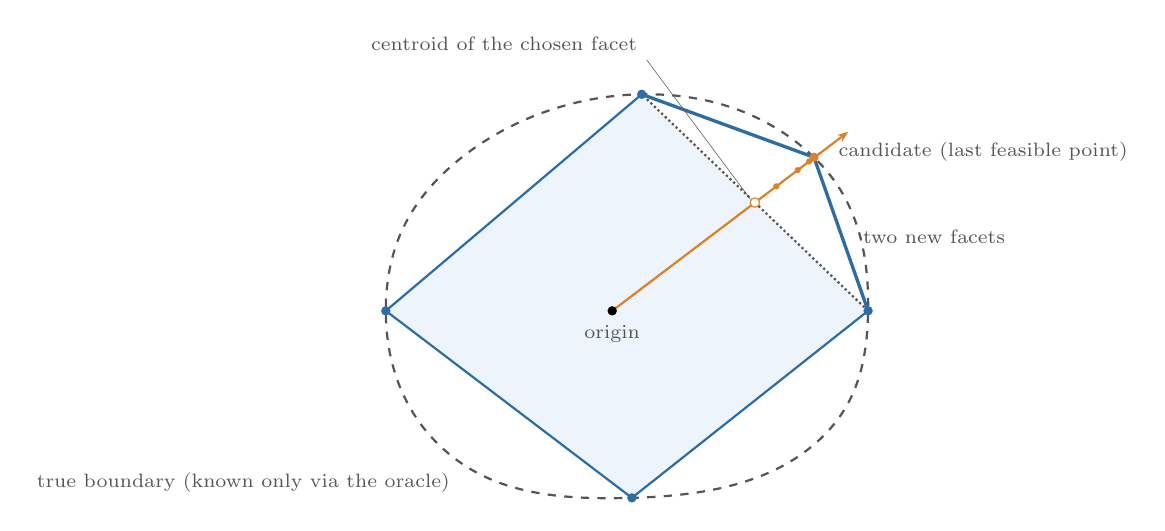
\begin{tikzpicture}[scale=1.25]
\draw[nbgrey, dashed, thick] plot[smooth cycle, tension=0.7] coordinates
  {(2.6,0) (2.05,1.56) (0.3,2.2) (-1.6,1.5) (-2.3,0) (-1.6,-1.5) (0.2,-1.9) (2.0,-1.4)};
\fill[notebg] (2.6,0) -- (0.3,2.2) -- (-2.3,0) -- (0.2,-1.9) -- cycle;
\draw[nbblue, thick] (0.3,2.2) -- (-2.3,0) -- (0.2,-1.9) -- (2.6,0);
\draw[nbgrey, thick, densely dotted] (2.6,0) -- (0.3,2.2);
\draw[nbblue, very thick] (2.6,0) -- (2.05,1.56) -- (0.3,2.2);
\draw[arr, draw=warnrule, thick] (0,0) -- (2.4,1.82);
\foreach \t in {1.15,1.3,1.38} \fill[warnrule] (1.45*\t,1.1*\t) circle (0.9pt);
\node[circle, fill=black, inner sep=1.2pt] at (0,0) {};
\node[lab, below] at (0,-0.05) {origin};
\node[circle, draw=warnrule, fill=white, inner sep=1.2pt] at (1.45,1.1) {};
\node[vtx] at (2.6,0) {}; \node[vtx] at (0.3,2.2) {}; \node[vtx] at (-2.3,0) {};
\node[vtx] at (0.2,-1.9) {}; \node[vtx, fill=warnrule] at (2.05,1.56) {};
\draw[nbgrey, very thin] (1.4,1.14) -- (0.35,2.55) node[lab, anchor=south east] {centroid of the chosen facet};
\node[lab, anchor=west] at (2.2,1.62) {candidate (last feasible point)};
\node[lab, anchor=west] at (2.45,0.75) {two new facets};
\node[lab, anchor=north east] at (-1.55,-1.55) {true boundary (known only via the oracle)};
\end{tikzpicture}
\caption{One step of the expansive loop in 2-D. The policy picks a facet
(dotted); bisection along the ray through its centroid finds the candidate,
which replaces the facet by $d$ new ones.}
\label{fig:expansive}
\end{figure}

\begin{lstlisting}
from OpenRC.region.expansive import ExpansiveBuilder

run = ExpansiveBuilder(
    policy="adaptive-gradient",       # which facet to break
    seed="random",                    # what to start from
    seed_kwargs={"n_samples": 2000, "batch_size": 500},
    n_workers="auto",
).build(case, axes, oracle,
        max_vertices=120,
        max_oracle_calls=20_000,
        max_seconds=600,
        memory_limit_mb=4096)

run.polytope, run.trace, run.oracle_stats, run.stopped_because
\end{lstlisting}

Oracle-call and time budgets count additional work from the beginning of this
build and are carried across memory-aware rounds. They are cooperative rather
than transactional: a ray bisection or random-seed batch already in progress
finishes before the next check. When an external service imposes a tight call
quota, keep the random seed's \code{batch\_size} below the remaining allowance.
A seed hull exceeding \code{max\_vertices} is reduced to that vertex budget,
with a warning. Greedy insertion starts from a large simplex and repeatedly
adds the vertex with the greatest volume gain; one matrix product scores all
candidates. In 5- to 8-D tests, the retained volume was within 2 percentage
points of greedy removal, with 100 to 1,000 times shorter execution time
(an 8-D seed of 1,010 vertices: 0.9\,s). \code{builder\_info["seed"]} records the
counts, the method and the volume lost. In \code{ExpansiveBuilder},
\code{max\_vertices} counts accepted boundary candidates (each requiring one
ray search), including points that become interior after subsequent insertions;
\code{RayGrowthBuilder} instead bounds the current hull vertex count.

\why{Boundary candidates are cached per facet. A surviving facet needs no
further boundary search, and nominations of the same facet by several policy
arms share one search. Table~\ref{tab:policies} reports the resulting search
counts.}

Throughout construction, the polytope is maintained in a single incremental
hull (\code{LiveHull}, Section~\ref{sec:livehull}): candidate volume gains are
evaluated directly from the visible facets, and accepted vertices are inserted
incrementally. Each step therefore requires one incremental update rather than
$2\times\text{arms}+1$ full hull reconstructions for
$\mathrm{vol}(V\cup p)-\mathrm{vol}(V)$, while producing identical vertices.
At termination the hull structure is released and only the vertex set is
retained, unless \code{keep\_hull=True} is specified.

\section{Facet-selection policies}
\label{sec:policies}

\file{OpenRC/region/facet\_policy.py}

Repeatedly selecting descendants of the same facet can concentrate exploration
in one part of the boundary, a Matthew effect. OpenRC provides four
single-measure policies and three adaptive policies, together with a random
baseline.

\begin{table}[h]
\centering\small
\caption{Expensive boundary searches per round, measured on \code{9bus}/\code{247}
with a 60-vertex budget. The facet queue averaged 41 entries.}
\label{tab:policies}
\begin{tabular}{@{}llr@{}}
\toprule
Policy & Rule & Searches/round \\
\midrule
\code{volume-gain}       & greedy: maximum realised hypervolume gain & 3.03 \\
\code{facet-area}        & largest facet $(d{-}1)$-volume            & 1.00 \\
\code{cone-volume}       & largest facet-to-origin cone              & 1.00 \\
\code{generation}        & oldest facet first                        & 1.00 \\
\code{random}            & uniform random selection (baseline)       & 1.00 \\
\code{adaptive-ema}      & full-information EMA bandit over the arms & 1.04 \\
\code{adaptive-egreedy}  & EMA plus $\varepsilon$ exploration        & 1.07 \\
\code{adaptive-gradient} & gradient bandit, arm sampled before reward& 1.00 \\
\bottomrule
\end{tabular}
\end{table}

\why{With caching, \code{volume-gain} requires one search per newly created
facet, or $d$ per break: the measured counts were 3.03, 4.03 and 8.06 at
$d = 3, 4, 8$. \code{adaptive-gradient} requires 1.00 search per round because
it samples an arm before evaluating its reward, then records the chosen
facet's realised gain in \code{observe}. The EMA policies evaluate each arm's
nomination.}

A cached gain is measured when its facet is first scored, and later insertions
can cover part of its added cap. Subsequent rankings can therefore use stale
gains. With \code{refresh\_gains=True}, the default of
\code{ExpansiveBuilder} and of the \code{facet-queue} and
\code{grow-and-polish} ray strategies, a queued facet's gain is re-measured on
the current hull from its cached boundary point, at no oracle cost. At equal
vertex counts this gives \code{volume-gain} $1.44\times$ (3-D), $1.63\times$
(5-D) and $107\times$ (8-D, 64 vertices) the volume of first-measurement
scoring; the adaptive policies are unaffected. \code{refresh\_gains=False}
scores as the published method did.
Refreshing adds geometry work without further oracle calls. Only gains
affected by an insertion are re-measured: a candidate that sees none of the
removed or created facets retains its gain. Facet areas are cached once
determinant evaluations have reached one per facet. In 8-D
(\code{volume-gain}, 120 vertices) refresh took 17.5\,s, against
5.8\,s without refresh and 74\,s re-measuring every gain, with the same
trajectory. \code{lazy=False} on an adaptive policy scores every queued facet,
as the unaccelerated method did: the same rule, at a higher search cost.

A policy can be preceded by a \textbf{screen}: step~1 of a two-step selection
decides which facets enter this iteration's pool, and the policy (step~2)
chooses within the pool only. The registered \code{debt} screen
(Section~\ref{sec:debt}) keeps facets that lie over vertices a compression
discarded out of the pool with high probability. Facet area and cone volume are
memoised per facet for the facet's lifetime, not per iteration, so a resumed
expansion over a hull of $10^5$ facets computes each measure once.

\section{Seeds and random acceleration}

\file{OpenRC/region/base.py}

\begin{center}\small
\begin{tabular}{@{}lp{9.9cm}@{}}
\toprule
\code{simplex} & $d+1$ rays: the unit axes plus one negative diagonal. \\
\code{axis}    & $2d$ signed axis rays; also yields an axis-intercept sampling box. \\
\code{random}  & The axis seed, plus $N$ uniform or Sobol points from that box;
  the feasible ones become vertices. \\
\bottomrule
\end{tabular}
\end{center}

The box spans the axis intercepts through the origin, not generally the entire
feasible set: coupled coordinates can allow points beyond these intercepts.

\label{sec:seeds}
The region CLI passes an explicit \code{--seed auto} unchanged to either
growth engine. Older ray-strategy CLI runs forced \code{axis} below 4-D;
use \code{--seed axis} explicitly to reproduce that trajectory.

\code{ExpansiveBuilder} defaults to \code{seed="auto"}: \code{axis} from 4-D up,
\code{simplex} in 3-D and below (\code{AXIS\_SEED\_FROM\_DIM}); a seed passed
explicitly is always used as given. The simplex seed uses the positive unit
axes and a single negative diagonal. Subsequent facet-centroid rays retain
this directional bias. Signed axis rays give a more symmetric initial coverage;
the measured volume ratios increase strongly with dimension:

\begin{center}\small
\begin{tabular}{@{}lrrrrrrr@{}}
\toprule
Dimension & 3 & 4 & 5 & 6 & 7 & 8 & 16 \\
\midrule
volume, axis / simplex seed & 1.3 & 3.8 & 21 & 101 & 3\,120 & 2\,410 & 27\,900 \\
\bottomrule
\end{tabular}
\end{center}
\noindent (\code{9bus}, AC oracle, \code{adaptive-ema}; 50 vertices up to 7-D,
60 in 8-D and 40 in 16-D; the oracle calls differ by under 20\,\%.) The
threshold of 4-D comes from the benchmark harness (Section~\ref{sec:benchmark}),
over random instances: 8 per network, P/Q axes, LinDistFlow. The axis seed gave
larger volumes in every 4-D instance, with a geometric-mean ratio to the
simplex seed of
2.3 on \code{9bus} and 38 on \code{pp:case33bw} at 20 vertices per dimension
(3.1 and 66 at 6 per dimension). It also gave larger volumes in all but one
3-D instance, by
1.16 and 4.4 (1.48 and 8.4). All intervals exclude 1. In 3-D \code{"auto"}
nevertheless keeps the simplex, so that the published low-dimensional results
reproduce. The 3-D comparisons also favour an explicit \code{seed="axis"}.

\why{A random feasibility test uses one oracle call, while a bisection needs
roughly thirty. Random sampling can therefore produce a coarse initial hull
with fewer calls than the same number of boundary searches.}

Large random starts are processed in bounded batches, each reduced to its hull
before the next is drawn. This preserves the final hull: a point interior to a
batch hull cannot be a vertex of the union hull.

\section{Memory-aware construction}
\label{sec:memaware}

\file{region/memory\_aware.py}, \file{compression/schedule.py},
\file{geometry/live\_hull.py} (all under \file{OpenRC/})

In high dimensions, combinatorial growth in the facet count can exhaust
memory before region construction converges (Table~\ref{tab:facetgrowth}).
\code{MemoryAwareBuilder} alternates expansion and compression on one live
hull. A configurable schedule determines when to compress and the stopping
criteria for compression.

\begin{table}[h]
\centering\small
\caption{Growth of a 16-D region (\code{9bus}, $P$ and $Q$ at all eight POCs,
\code{acpf}, \code{generation} policy). Two more vertices roughly double the
facets, with little additional volume.}
\label{tab:facetgrowth}
\begin{tabular}{@{}rrrrr@{}}
\toprule
Vertices & Facets & Volume & Process RSS & Hull build \\
\midrule
28 & 7\,590     & 1.06 & 354\,MiB   & 0.01\,s \\
32 & 56\,021    & 1.60 & 469\,MiB   & 0.16\,s \\
36 & 105\,537   & 2.22 & 605\,MiB   & 0.46\,s \\
40 & 534\,283   & 2.23 & 1\,134\,MiB & 2.54\,s \\
42 & 959\,086   & 2.23 & 1\,822\,MiB & 5.08\,s \\
\bottomrule
\end{tabular}
\end{table}

\subsection{Incremental hull operations}
\label{sec:livehull}

A \code{LiveHull} keeps one incremental Qhull object alive from the seed to the
last compression and supports the following operations:

\begin{center}\small
\begin{tabular}{@{}l>{\raggedright\arraybackslash}p{10.2cm}@{}}
\toprule
\code{gain(p)} & Exact added volume evaluated without invoking Qhull,
  $\sum_{F\ \text{visible from}\ p} |\det(F-p)|/d!$ over the triangulated
  visible facets. \\
\code{add(p)} & Qhull incremental insertion, updating only visible facets.
  Insertions nearly coplanar with an existing facet are cross-checked against
  \code{gain(p)} and trigger a full rebuild on mismatch (see below). \\
\code{marginal\_loss(i)} & $\mathrm{vol}(\mathrm{conv}(N_i\cup v_i)) -
  \mathrm{vol}(\mathrm{conv}(N_i))$, with $N_i$ the vertices sharing a facet with
  $v_i$ (two small hulls in 3-D, or one full rebuild in high dimensions when
  $N_i$ spans most of the vertex set). \\
\code{star\_volumes()} & Sum of centroid-to-facet cone volumes incident to each
  vertex (an upper bound on marginal loss, computed for all vertices in one pass). \\
\code{remove(i)} & Full hull rebuild upon vertex deletion (Qhull does not
  support incremental deletion), executed only for accepted removals. \\
\bottomrule
\end{tabular}
\end{center}

\why{Deleting $v_i$ changes only its adjacent facets. Their replacements are
the facets of $\mathrm{conv}(N_i)$ visible from $v_i$, so the removed cap is
the volume $v_i$ adds to $\mathrm{conv}(N_i)$. The local calculation agrees
with full rebuilds to
$10^{-15}$ in 2- to 6-D, including coplanar facets. It also makes the
incremental update exact: removing $v_j$ leaves $N_i$ unchanged unless $i$ and
$j$ are neighbours.}

\trap{Qhull can report an incorrect incremental volume when a new point is
coplanar with an existing facet while exterior to it: Qhull extends that facet
but retains its previous area. Reported volumes have been up to 60\,\% too
small, below the pre-insertion volume, with the error persisting across
subsequent insertions. This occurs mainly with box-shaped or grid-like point
sets and is uncommon in growth from ray boundaries. \code{add} therefore
compares nearly coplanar insertions (distance to a facet plane within
$10^{-9}$ of the coordinate scale) against \code{gain(p)} and rebuilds the hull
on mismatch. Across approximately 20\,700 degenerate insertions in 2- to 6-D,
all volumes matched full rebuilds; non-degenerate builds incur no runtime
overhead and yield identical hulls.}

Memory is modelled as $40d+108$ bytes per facet (Qhull's facet record plus
SciPy's arrays; measured 443--538\,B in 8-D and 690\,B in 16-D). A builder
returns the vertex set only; its volume is filled in from the hull, and the hull
is released.

\subsection{Compression schedules}

\begin{center}\small
\begin{tabular}{@{}lp{10.4cm}@{}}
\toprule
\code{"vertex-budget"} & The published rule, and the default: grow to
  \code{max\_vertices} ($M$), compress to \code{target\_vertices} ($\hat M$).
  The same vertex thresholds apply in every dimension. \\
\code{"memory-budget"} & At \code{high\_water}$\times$\code{budget\_mb}, compress
  until the live hull's \emph{measured} memory is under
  \code{low\_water}$\times$\code{budget\_mb}. \\
\code{"adaptive"} & \code{memory-budget}, with a per-removal loss limit and a
  stopping rule estimated from recent growth (Section~\ref{sec:adaptive}). \\
\code{None} & Never compress. \\
\bottomrule
\end{tabular}
\end{center}

The compressor defaults to \code{"auto"}: \code{local-search} up to 6-D and
\code{star-screened} above, where it is 3.2--3.9$\times$ faster in 7- and 8-D at
volume ratios 0.93--1.12; pass \code{compressor="local-search"} for exact greedy
in every dimension.

\begin{lstlisting}
from OpenRC.region.memory_aware import MemoryAwareBuilder

MemoryAwareBuilder(compressor="auto",               # star-screened above 6-D
                   schedule="adaptive", schedule_kwargs={"budget_mb": 80},
                   refiner="relocation",             # optional: move vertices
                   max_vertices=10_000, rounds=40)

# custom schedule subclass (registration optional)
from OpenRC.compression import CompressionPlan, CompressionSchedule

class EveryTenSteps(CompressionSchedule):
    def decide(self, state):                         # called every iteration
        if state.iteration >= 10:
            return CompressionPlan(max_volume_loss_pct=0.5, reason="ten steps")
        return None
MemoryAwareBuilder(schedule=EveryTenSteps())
\end{lstlisting}

A schedule receives a \code{GrowthState} each iteration: hull vertices, facets,
modelled memory, process RSS, volume, oracle calls, time, and the growth trace
since the last compression. These quantities are available without rebuilding
the hull. The schedule returns \code{None} or a \code{CompressionPlan}, whose four fields are
stopping rules of \code{Compressor.compress\_live}: a vertex target, a cumulative
loss budget, a memory goal and a per-removal price. Whichever binds first ends
the compression. Registering with \code{@SCHEDULES.register} additionally makes
it available by name.

\begin{figure}[htbp]
\centering
\resizebox{\textwidth}{!}{%
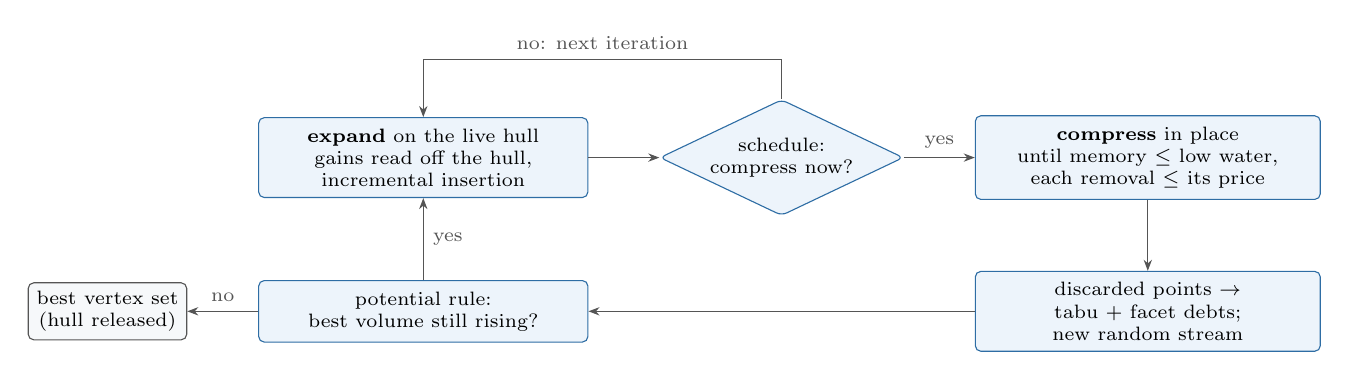
\begin{tikzpicture}[node distance=6mm and 9mm]
\node[blk, text width=3.9cm] (grow) {\textbf{expand} on the live hull\\gains read off the hull,\\incremental insertion};
\node[blk, diamond, aspect=2.1, inner sep=1pt, right=of grow] (ask) {schedule:\\compress now?};
\node[blk, text width=4.1cm, right=of ask] (comp) {\textbf{compress} in place\\until memory $\le$ low water,\\each removal $\le$ its price};
\node[blk, text width=4.1cm, below=9mm of comp] (carry) {discarded points $\rightarrow$\\tabu + facet debts;\\new random stream};
\node[blk, text width=3.9cm] (stop) at (grow |- carry) {potential rule:\\best volume still rising?};
\node[res, left=9mm of stop] (out) {best vertex set\\(hull released)};
\draw[arr] (grow) -- (ask);
\draw[arr] (ask) -- node[lab, above] {yes} (comp);
\draw[arr] (ask.north) -- ++(0,5mm) -| node[lab, pos=0.25, above] {no: next iteration} (grow.north);
\draw[arr] (comp) -- (carry);
\draw[arr] (carry) -- (stop);
\draw[arr] (stop) -- node[lab, right] {yes} (grow);
\draw[arr] (stop) -- node[lab, above] {no} (out);
\end{tikzpicture}}
\caption{The memory-aware cycle. Every stage works on the same hull; only the
vertex set leaves the builder.}
\label{fig:memaware}
\end{figure}

\subsection{Adaptive compression criteria}
\label{sec:adaptive}

\begin{enumerate}
\item \textbf{Compression trigger.} The live hull reaches \code{high\_water} (0.9) of
  \code{budget\_mb}; or the process RSS reaches \code{rss\_high\_water} of the
  run's \code{memory\_limit\_mb}; or the expansion hits \code{max\_vertices}.
\item \textbf{Memory target.} Remove vertices until the hull's memory,
  measured after every removal, is under \code{low\_water} (0.5) of the budget.
  Compression changes the relation between vertex and facet counts, making a
  growth-based memory prediction unreliable. In 8-D, 108$\to$92 vertices freed
  10\,\% of memory, while a fit based on the growth trajectory predicted 45\,\%.
\item \textbf{Per-removal loss limit.} A vertex is removed only if it costs at most
  $\ell_{\max} = \mathrm{payback}\cdot g$, where $g$ is the volume a new vertex
  currently adds (\code{payback} 0.5). Greedy compressors remove the cheapest
  vertex first, so compression stops when the next removal exceeds the allowed
  share of estimated growth.
\item \textbf{Growth estimate.} The volume gains $y_t$ of accepted vertices
  are modelled as noisy observations of a slowly varying mean $g_t$ under the
  local-level state-space model $g_t = g_{t-1}+w_t$, $y_t = g_t+e_t$. Its
  Kalman filter converges to
  $\hat g_t = \hat g_{t-1} + \eta\,(y_t-\hat g_{t-1})$ with
  $\eta = 2/(\text{window}+1)$, bias-corrected for its zero initialisation. The
  filter state persists across rounds, preserving the estimate even when an
  expansion phase terminates after a single insertion.
\item \textbf{Termination.} Stop after a compression that could not free
  \code{min\_free} vertices at a profitable price, or by the potential rule: the
  best volume $\Phi_k$ after round $k$ never falls and is bounded by the true
  region's volume $V^\ast$, so requiring a rise of \code{round\_tol} every
  \code{patience} rounds ends any run within
  $\mathrm{patience}\cdot(\lceil \ln(V^\ast/\Phi_0)/\ln(1+\mathrm{round\_tol})\rceil+1)$
  rounds. This rule excludes indefinitely repeated states with constant $\Phi$.
\item \textbf{Between rounds.} Round $r$ draws from its own stream, derived from
  $(\text{seed}, r)$ by \code{numpy.random.SeedSequence}: independent of the other
  rounds and independently reproducible. Discarded vertices are marked
  \emph{tabu} (excluded from re-insertion in the subsequent expansion) and
  contribute to facet debts (Section~\ref{sec:debt}). Boundary searches are
  cached by ray direction, so a facet that
  survives a compression costs no oracle call when it is explored again.
\end{enumerate}

\trap{Resetting every round to the same random seed repeats round~0's
tie-breaks. On the 16-D region, the builder then repeatedly added and removed
the same two vertices for eight rounds. The current implementation carries
the tabu set and uses a new stream each round. Returning to an earlier vertex
set alone does not establish a cycle; termination follows the potential rule.}

\subsection{Two-step facet selection: debts}
\label{sec:debt}

A discarded vertex $v$ lies beyond the facets of the compressed hull it can see,
and the cap it cut off is the union of the cones $\mathrm{conv}(F,v)$ over those
facets. Further exploration of these facets can recover points that compression
has already discarded. With \code{facet\_screen="debt"} (off by default):

\begin{enumerate}
\item every facet is charged a \emph{debt}: by default the number of discarded
  vertices that lie beyond it; with the \code{cone} weighting, one unit for the
  facet a vertex sits over most and $\mathrm{cone}(F,v)/\max\mathrm{cone}$ for
  the others;
\item step~1 keeps a facet in this iteration's pool with probability
  $\pi(F) = \max\bigl(e^{-\mathrm{debt}(F)/\tau},\ \pi_{\min}\bigr)$, with
  $\tau = 0.5$ and $\pi_{\min} = 0.01$: debt reduces selection probability
  without excluding a facet permanently;
\item step~2 is the ordinary policy, choosing within the pool;
\item a broken facet passes \code{inheritance}$\times$debt (0.8) to each child:
  its descendants therefore retain part of the selection penalty.
\end{enumerate}

Debt-free facets are always kept and cost no random draw, so a run without
discarded points is bit-for-bit the same with or without the screen. Screens are
a registry (\code{FACET\_SCREENS}); a new one implements \code{pool(debts, rng)}.

The screen's effect depends on the seed. With the one-sided simplex seed, it
increased the 8-D adaptive result from $+48$\,\% to $+85$\,\%; with the axis seed
(the default in 8-D) its effect is within the spread between random seeds:

\begin{center}\small
\begin{tabular}{@{}lrrrr@{}}
\toprule
8-D, 16\,MiB, gain over the first expansion & seed 0 & seed 1 & seed 2 & mean \\
\midrule
\code{adaptive}, no screen         & +26.3\,\% & +40.8\,\% & +27.5\,\% & +31.5\,\% \\
\code{adaptive} + debt (count)     & +19.3\,\% & +23.6\,\% & +31.2\,\% & +24.7\,\% \\
\code{adaptive} + debt (cone)      & +39.8\,\% & +45.2\,\% & +27.3\,\% & +37.4\,\% \\
\bottomrule
\end{tabular}
\end{center}

\subsection{Dimension-dependent effects of debt screening}
\label{sec:debtfade}

Measurements from resumed adaptive rounds characterise the effects of seed
coverage, debt screening and vertex placement:

\begin{center}\small
\begin{tabular}{@{}lrrr@{}}
\toprule
& \multicolumn{2}{c}{8-D, 16\,MiB} & 16-D, 80\,MiB \\
\cmidrule(lr){2-3}\cmidrule(l){4-4}
& simplex seed & axis seed & simplex seed \\
\midrule
vertices per dimension at the budget, $N/d$      & 13.5         & 13.9        & 2.25 \\
facets a discarded vertex can see               & 2.6--4.5\,\% & 0.6--2.9\,\% & 10.6--24.6\,\% \\
inserted points kept by the next compression    & 58--100\,\%  & 50--78\,\%  & 0\,\% \\
\bottomrule
\end{tabular}
\end{center}

\begin{enumerate}
\item \textbf{Seed coverage.} The simplex seed left many directions
  unexplored. Debt screening helped direct resumed expansions towards these
  directions. With the broader coverage of the axis seed, its effect was
  approximately neutral.
\item \textbf{Facet visibility.} With $N$ close to $2d$, the hull is nearly
  neighbourly, with a facet count near McMullen's upper bound
  $O(N^{\lfloor d/2\rfloor})$. A point just outside the 16-D hull sees a
  quarter of its facets, reducing the selectivity of the debt measure.
\item \textbf{Marginal volume.} In the 16-D runs, a new vertex added a fifth
  to two fifths of the volume retained by an established vertex. All points
  inserted by resumed expansions were removed at the next compression.
  The axis seed alone (32 vertices, $2^{16}$ facets) uses 58\,\% of an
  80\,MiB budget, and no further insertion recovered the required removal
  loss within that budget.
\item \textbf{Vertex placement.} The best inscribed
  polytope with $N$ vertices approaches the region as $N^{-2/(d-1)}$
  (Gruber's theorem, giving an exponent of $0.13$ in 16-D), so a
  memory-bounded $N$ remains far from the asymptotic regime. Refinement
  improves vertex placement within this fixed cardinality.
\end{enumerate}

\subsection{Refinement by vertex relocation}
\label{sec:refine}

\file{OpenRC/region/refine.py}

A \textbf{refiner} improves the live hull at a fixed vertex count. The
registered \code{relocation} is first-order local search for the
maximum-volume $N$-vertex polytope inscribed in the region. With the hull
triangulated into cones $\mathrm{conv}(c, F)$, each of volume
$V_F = |\det D_F|/d!$, Jacobi's formula gives the exact volume gradient of every
vertex at once:
\begin{equation}
\nabla_{v_i}\mathrm{vol} = \sum_{F \ni i} V_F\,\bigl(D_F^{-\top}\bigr)_{\text{row of } i}.
\end{equation}
A vertex must stay on the boundary, so only the gradient's component tangent to
the sphere of directions can be followed. A move selects the vertex with the
largest predicted gain, rotates its direction by its step angle towards the
tangent gradient,
finds the boundary point on that ray (one bisection), and accepts the
replacement only when it increases hypervolume within the memory cap,
preserving both vertex count and monotonicity. Each vertex maintains an
individual step size adapted via Rechenberg's $1/5$ success rule, and the
search terminates once all step sizes fall below \code{min\_step}. At that
angular resolution, this corresponds to \emph{Property~Z} (local volume
stationarity under single-vertex boundary perturbations), which is a necessary
condition for a maximum-volume inscribed polytope rather than a global
optimality guarantee.

\begin{lstlisting}
MemoryAwareBuilder(schedule="adaptive", schedule_kwargs={"budget_mb": 80},
                   refiner="relocation", refine_moves=None)   # None: 2 x vertices

# or on any stored region, at its own size
from OpenRC.region.refine import get_refiner
better, info = get_refiner("relocation").refine_polytope(region, oracle, axes)
\end{lstlisting}

Refiners are registered in \code{REFINERS}. An implementation provides
\code{refine(live, oracle, axes, ...)}, must never let the volume fall, and can
be passed as an instance. Refinement is disabled by default.

The measured benefit was largest at small $N/d$. In 16-D under 80\,MiB,
the axis seed allowed no further profitable insertion, while relocation
increased volume:
$+12.8$\,\% after the adaptive schedule (880 oracle calls) and $+55$\,\% as
the polishing stage of \code{grow-and-polish} with 400 moves (3\,412 calls;
Section~\ref{sec:rays}). In 8-D, refinement added little beyond compression
and regrowth ($+22.4$\,\% against $+22.3$\,\% for 12\,112 against 2\,373 calls). A
move costs one hull rebuild, which in 16-D grows with the facet count: about
2\,s at 32 vertices, 50\,s at 40. An optional first-order screen,
$\nabla_{v_i}\mathrm{vol}\cdot(p - v_i) \le 0$, can skip that rebuild, but it is
only a speed heuristic: the derivative holds the current facet structure fixed,
whereas a finite step may alter facet incidence and still increase hypervolume
(in 2-D, a move with a negative directional derivative can still increase exact
area by 22\,\%). Consequently
\code{first\_order\_screen=False} is the default in ray growth and relocation;
enable it when the measured speed/quality trade-off is acceptable.

\paragraph{Parallel move evaluation.} Several candidate replacements can be
evaluated together. With \code{batch=k} (on
\code{RayGrowthBuilder}, \code{GradientRelocation} and \code{run\_rays}), the
strategy proposes up to $k$ moves from the same state (\code{propose\_batch};
gradient moves for the $k$ most promising vertices). The engine fires their
rays, measures the $k$ replacement hulls in threads and applies the best
acceptable one; the others are reported as \code{"outranked"}, which the
gradient strategy treats as neutral. A strategy without \code{propose\_batch}
proposes one move at a time. In 8-D, \code{grow-and-polish} is
2.0--2.8 times faster at the same number of oracle calls (the move budget counts
proposals), and its volumes change by $-1.2$ to $+4.5\,\%$. The default,
\code{batch=1}, fires one ray at a time.

\subsection{Memory-budget comparisons}

\noindent\begin{minipage}{\linewidth}
\begin{center}\small
\captionof{table}{Growing under a live-hull memory budget on \code{9bus} with the AC
oracle, the \code{adaptive-ema} policy and the default (axis) seed. 8-D: $P$ at
all eight POCs, 16\,MiB; 16-D: $P$ and $Q$ at all eight, 80\,MiB. The 16-D
polish is sensitive to rounding (\code{numba=False}: 17\,691).
$^\ast$\,$M/\hat M$ = 78/58 in 8-D and 36/34 in 16-D; the vertex-budget rule is
independent of the memory limit.}
\label{tab:memaware}
\begin{tabular}{@{}lrrrrrr@{}}
\toprule
& \multicolumn{3}{c}{8-D, 16\,MiB} & \multicolumn{3}{c}{16-D, 80\,MiB} \\
\cmidrule(lr){2-4}\cmidrule(l){5-7}
& volume & calls & peak MiB & volume & calls & peak MiB \\
\midrule
grow to the budget, no compression & $4.08\cdot10^7$ & 1\,508 & 14.5 & 10\,812 & 388 & 46.8 \\
\code{vertex-budget}$^\ast$        & $2.29\cdot10^7$ & 2\,906 & 14.0 & 38\,719 & 672 & \textbf{433.2} \\
\code{adaptive}                    & $5.00\cdot10^7$ & 2\,373 & 14.7 & 10\,812 & 388 & 46.8 \\
\code{adaptive} + debt + relocation & $5.00\cdot10^7$ & 12\,112 & 14.8 & 12\,193 & 880 & 46.8 \\
\code{ray-growth}, \code{grow-and-polish} & $3.88\cdot10^7$ & 4\,094 & 15.9 & \textbf{16\,800} & 3\,412 & 46.8 \\
\bottomrule
\end{tabular}
\end{center}
\end{minipage}


\why{In the 8-D comparison, compression and regrowth within 16\,MiB increased
volume by $+22$\,\%; the published vertex-budget rule reduced it by 44\,\%.
In 16-D, the seed allowed no further profitable insertion within the budget,
so the adaptive schedule stopped immediately. Relocation increased volume
by $+55$\,\% with \code{grow-and-polish}. The vertex-budget rule obtained
$3.6\times$ the volume using $5.4\times$ the memory. Reproduce with
\code{python scripts/benchmark\_memory.py}.}

\section{Ray strategies}
\label{sec:rays}

\file{OpenRC/region/ray\_growth.py}

Ray-based growth selects a direction, locates its boundary point by bisection,
and decides whether to add or replace a vertex. \code{ExpansiveBuilder}
specifies the direction and update rules together.
\code{RayGrowthBuilder} (registered as \code{ray-growth}) separates them:

\begin{itemize}
\item a \textbf{ray strategy} proposes a \code{RayProposal} specifying a
  direction, an update action (\code{replace=None} for insertion or
  \code{replace=i} for vertex replacement) and an optional boundary-distance
  \code{hint}, and receives the resulting \code{RayOutcome};
\item the \textbf{engine} performs the cached, hint-initialised ray search,
  evaluates the exact candidate volume on the live hull, applies the acceptance
  criterion (strict volume increase by default) together with the vertex and
  hull-memory caps, and retains the highest-volume hull encountered across the
  run.
\end{itemize}

The cap concerns modelled live-hull memory, not process RSS. Both builders and
\code{run\_rays} reject a starting hull already above \code{max\_hull\_mb},
including a zero-move run, with \code{MemoryBudgetExceeded}. They release a
rejected hull they created, but leave a supplied \code{initial\_hull} usable.
Seed construction happens before its footprint can be measured; temporary
seed/Qhull allocations are not bounded by this test. Both region CLI growth
paths forward \code{--max-hull-mb}; an impossible cap fails before saving.

\begin{center}\small
\begin{tabular}{@{}l>{\raggedright\arraybackslash}p{10.6cm}@{}}
\toprule
\code{facet-queue} & The expansive builder's virtual facet queue with any
  facet-selection policy: facet breaking as a ray strategy. \\
\code{facet} & The best real facet of the live hull by a score: gain predicted
  from the vertex radii (default), cone volume, area, or a custom function; with
  \code{lookahead=k} the $k$ best are probed and the largest realised gain is used. \\
\code{gradient} & Relocation moves (Section~\ref{sec:refine}) plus
  Linde--Buzo--Gray splitting: while the budget has room, the most promising
  vertex is split into itself and a rotated copy. \\
\code{relocation} & The moves only: improvement at a fixed vertex count. \\
\code{grow-and-polish} & \code{facet-queue} until the vertex or memory cap,
  followed by \code{relocation} (default). \\
\bottomrule
\end{tabular}
\end{center}

\begin{lstlisting}
from OpenRC.region.ray_growth import RayGrowthBuilder, RayProposal, RayStrategy

RayGrowthBuilder(strategy="grow-and-polish").build(
    case, axes, oracle, max_vertices=60, max_hull_mb=16, max_moves=240)

class RandomDirections(RayStrategy):            # custom ray strategy
    def propose(self, ctx):                     # None: nothing left to try
        if not ctx.room:
            return None
        return RayProposal(direction=ctx.rng.normal(size=ctx.dim))

RayGrowthBuilder(strategy=RandomDirections())
\end{lstlisting}

A strategy reads a \code{RayContext}: the live hull, vertex radii and
directions, the exact volume gradient and its tangential part, facet
directions, origin cones and predicted gains (each computed at most once per
hull state), together with \code{ctx.boundary(direction, hint)}, a probe through the
engine's ray cache that counts towards every budget. \code{SequentialRays}
chains strategies (each runs until it returns \code{None}); \code{accept} can
be overridden, for instance for simulated annealing. Registering with
\code{@RAY\_STRATEGIES.register} makes a strategy available by name. The engine
rejects proposals with non-finite directions or out-of-range vertex indices.

Without a memory budget, at a fixed vertex count (\code{9bus}, AC oracle,
default seed):

\begin{center}\small
\begin{tabular}{@{}lrrrr@{}}
\toprule
& \multicolumn{2}{c}{8-D, 60 vertices} & \multicolumn{2}{c}{16-D, 40 vertices} \\
\cmidrule(lr){2-3}\cmidrule(l){4-5}
& volume & calls & volume & calls \\
\midrule
\code{ExpansiveBuilder}, \code{adaptive-ema} & $3.28\cdot10^6$ & 1\,503 & 65\,822 & 924 \\
\code{ray-growth}, \code{facet-queue}         & $4.44\cdot10^6$ & 1\,296 & 65\,564 & 884 \\
\code{ray-growth}, \code{grow-and-polish}     & $6.62\cdot10^6$ & 5\,122 & 155\,190 & 3\,816 \\
\bottomrule
\end{tabular}
\end{center}

In these comparisons, the facet queue inside the ray engine obtained more
volume with fewer calls through warm-started bisections and a budget applied
only to hull vertices; candidates adding no volume were discarded. Subsequent
polishing doubled the 8-D volume and increased the 16-D volume by a factor of
2.4. The \code{gradient} strategy alone produced $3.4\cdot10^5$ in 8-D for
6\,024 calls, substantially below the facet queue. These results favour the
facet queue's broader directional coverage over local moves during growth.

%==============================================================================
\chapter{Conservative construction}
\label{ch:conservative}

An inner approximation requires every point of the region to be feasible for
the exact model. Feasibility under a linearised model alone does not establish
this property.

OpenRC provides two conservative constructions based on intersections of
convex model regions. They use different model pairs, and Method~1 includes
a loss-shift step. Their guarantees depend on the loss-coverage conditions
described below; other configurations require certification.

\begin{center}
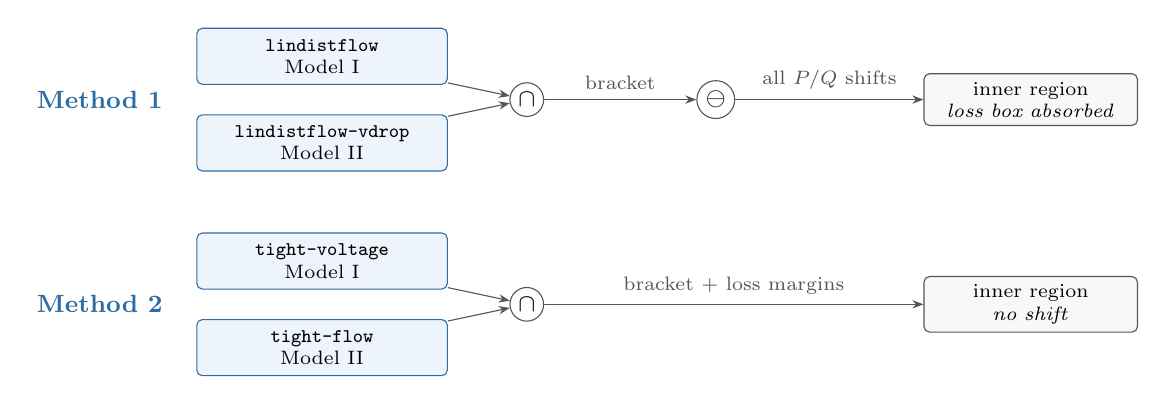
\begin{tikzpicture}[
  m/.style={blk, text width=2.9cm},
  op/.style={draw=nbgrey, fill=white, circle, font=\small, inner sep=1.5pt},
  r/.style={res, text width=2.5cm},
  ti/.style={font=\small\bfseries, color=nbblue, anchor=east}]
\node[ti] at (-1.9,1.3) {Method 1};
\node[m] (a1) at (0,1.85) {\texttt{lindistflow}\\Model~I};
\node[m] (b1) at (0,0.75) {\texttt{lindistflow-vdrop}\\Model~II};
\node[op] (i1) at (2.6,1.3) {$\cap$};
\node[op] (s1) at (5.0,1.3) {$\ominus$};
\node[r]  (o1) at (9.0,1.3) {inner region\\\emph{loss box absorbed}};
\draw[arr] (a1) -- (i1); \draw[arr] (b1) -- (i1);
\draw[arr] (i1) -- node[lab, above]{bracket} (s1);
\draw[arr] (s1) -- node[lab, above]{all $P/Q$ shifts} (o1);
\node[ti] at (-1.9,-1.3) {Method 2};
\node[m] (a2) at (0,-0.75) {\texttt{tight-voltage}\\Model~I};
\node[m] (b2) at (0,-1.85) {\texttt{tight-flow}\\Model~II};
\node[op] (i2) at (2.6,-1.3) {$\cap$};
\node[r]  (o2) at (9.0,-1.3) {inner region\\\emph{no shift}};
\draw[arr] (a2) -- (i2); \draw[arr] (b2) -- (i2);
\draw[arr] (i2) -- node[lab, above]{bracket + loss margins} (o2);
\end{tikzpicture}
\end{center}

\section{Method 1: \code{intersect-shift}}
\label{sec:method1}

Models: \code{lindistflow} (Model~I) and \code{lindistflow-vdrop} (Model~II).

\begin{enumerate}
\item Intersect the two regions, $\bar{C} = C^{I} \cap C^{II}$. They bracket
  the voltage-loss term.
\item Both models omit losses from the power balance. The exact model
  adds $r\,l$ to every branch's active flow and $x\,l$ to its reactive
  flow simultaneously, with $l \in [0, l^{max}]$. For every POC $j$
  the region is shifted along $P_j$ by $r_{ij} l^{max}_{ij}$ and along $Q_j$
  by $x_{ij} l^{max}_{ij}$, and a point is kept only if it stays in $\bar{C}$
  under every combination of these shifts, covering the full loss box:
  \begin{equation}
  R \;=\; \bigcap_{\delta \in \text{corners of the off-axis box}}
    \Bigl( \bar{C}(\delta) \ominus [0, s] \Bigr).
  \end{equation}
\item Optionally clip to each POC's own rating.
\end{enumerate}

Here $s$ collects the shifts along directions that are axes of the region,
and $\ominus [0, s]$ is the Pontryagin difference with their box
(\code{erode\_by\_box}). $\bar{C}(\delta)$ is the \emph{slice} of the feasible
set with the base injection raised by $\delta$. Off-axis shifts, such as a
$Q_j$ shift in an active-power region, require both component regions to be
rebuilt at that base through \code{OffsetOracle}. With $k$ off-axis directions,
the construction requires $2^k$ slice builds; a 4-D region over active power
needs 16. Figure~\ref{fig:method1}
shows both operations.

\begin{figure}[htbp]
\centering
\begin{subfigure}[t]{0.49\textwidth}
\centering
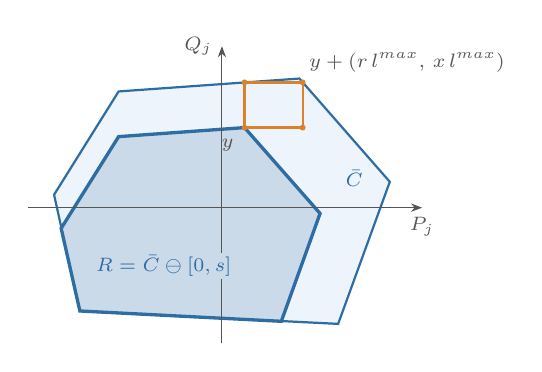
\begin{tikzpicture}[scale=0.82]
\filldraw[fill=notebg, draw=nbblue, thick]
  (-2.20,-1.60) -- (1.80,-1.80) -- (2.60,0.40) -- (1.20,2.00) -- (-1.60,1.80) -- (-2.60,0.20) -- cycle;
\filldraw[fill=nbblue!25, draw=nbblue, very thick]
  (-2.49,-0.32) -- (-2.20,-1.60) -- (0.92,-1.76) -- (1.52,-0.09) -- (0.35,1.24) -- (-1.60,1.10) -- cycle;
\draw[axis] (-3,0) -- (3.1,0) node[lab, below] {$P_j$};
\draw[axis] (0,-2.1) -- (0,2.5) node[lab, left] {$Q_j$};
\draw[warnrule, thick] (0.35,1.24) rectangle (1.25,1.94);
\foreach \p in {(0.35,1.24),(1.25,1.24),(0.35,1.94),(1.25,1.94)} \fill[warnrule] \p circle (1.3pt);
\node[lab, anchor=north east] at (0.33,1.22) {$y$};
\node[lab, anchor=south west] at (1.2,1.95) {$y + (r\,l^{max},\,x\,l^{max})$};
\node[font=\scriptsize, color=nbblue, fill=nbblue!25, inner sep=1pt] at (-0.9,-0.9) {$R = \bar C \ominus [0,s]$};
\node[font=\scriptsize, color=nbblue] at (2.05,0.45) {$\bar C$};
\end{tikzpicture}
\caption{On-axis shifts: $y$ is retained only if all four corners of its loss
box lie in $\bar C$. The dark region is the Pontryagin difference.}
\end{subfigure}\hfill
\begin{subfigure}[t]{0.49\textwidth}
\centering
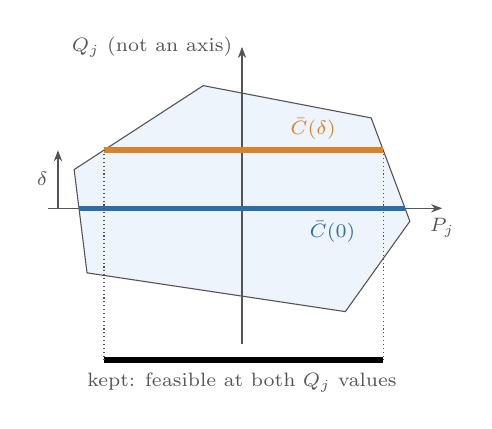
\begin{tikzpicture}[scale=0.82]
\filldraw[fill=notebg, draw=nbgrey]
  (-2.40,-1.00) -- (1.60,-1.60) -- (2.60,-0.20) -- (2.00,1.40) -- (-0.60,1.90) -- (-2.60,0.60) -- cycle;
\draw[axis] (-3,0) -- (3.1,0) node[lab, below] {$P_j$};
\draw[axis] (0,-2.1) -- (0,2.5) node[lab, left] {$Q_j$ (not an axis)};
\draw[nbblue, line width=2pt] (-2.525,0) -- (2.525,0);
\draw[warnrule, line width=2pt] (-2.138,0.9) -- (2.188,0.9);
\draw[arr, thick] (-2.85,0) -- node[lab, left] {$\delta$} (-2.85,0.9);
\node[font=\scriptsize, color=nbblue, anchor=north] at (1.4,-0.05) {$\bar C(0)$};
\node[font=\scriptsize, color=warnrule, anchor=south] at (1.1,0.92) {$\bar C(\delta)$};
\draw[black, line width=2pt] (-2.138,-2.35) -- (2.188,-2.35);
\draw[densely dotted, nbgrey] (-2.138,0.9) -- (-2.138,-2.35) (2.188,0.9) -- (2.188,-2.35);
\node[lab, anchor=north] at (0,-2.4) {kept: feasible at both $Q_j$ values};
\end{tikzpicture}
\caption{Off-axis shift: the original region is a slice at the base $Q_j$.
Raising $Q_j$ by $\delta = x\,l^{max}$ gives a second slice, rebuilt with
\code{OffsetOracle}; the retained region is their intersection.}
\end{subfigure}
\caption{The two operations of Method~1, drawn for one POC $j$.}
\label{fig:method1}
\end{figure}

\begin{lstlisting}
ConservativeBuilder(method="intersect-shift",
                    shift_scope="path")    # the default
\end{lstlisting}

\why{The shift operations have an exact inequality representation. A copy of
$\{Ay \le b\}$ shifted by $-t$ is $\{Ay \le b - At\}$. Requiring every
corner of the box tightens each row by its worst corner,
$\sum_k \max(0, a_k s_k)$. The rows of all slices are stacked, and the vertices
are enumerated once, by \code{from\_halfspaces}. The result carries those
inequalities as its exact \code{hrep}.}

\subsection{Loss-shift scope}
\label{sec:shiftscope}

\code{shift\_scope} selects the branches whose losses contribute to each shift:

\begin{description}
\item[\code{"path"} (default)] every branch from the POC to the slack.
\item[\code{"feeding\_branch"}] only the branch feeding the POC. This is exact
  when every bus is a POC.
\end{description}

\trap{On a reduced set of POC coordinates, \code{feeding\_branch} can miss a
downstream POC's load on an upstream branch whose loss no retained coordinate
carries. For example, on \code{9bus} (axes \code{247}), the two points
$(-0.853, 0.967, 3.945)$ and $(3.691, 0.378, 4.186)$\,MW lie inside the
direct-feeder region of the original scripts yet overload \code{Line 8-3} to
\textbf{101.07\%}. Both AC power flow and the exact Gurobi
model confirm they are infeasible, and both lie outside the \code{path}
region. The certificate refutes
the direct-feeder scope on 4-D regions as well (Table~\ref{tab:certificate}).
Neither scope is labelled theorem-backed when the selected axes omit buses
whose branch losses must be represented.}

\section{Method 2: \code{tight-intersect}}
\label{sec:method2}

Models: \code{tight-voltage} (Model~I) and \code{tight-flow} (Model~II),
intersected directly.

\begin{lstlisting}
ConservativeBuilder(method="tight-intersect")
\end{lstlisting}

Model~I includes the upper voltage-loss term and path-tightened thermal bounds;
Model~II includes maximum balance losses and the nameplate thermal bound.
Their direct intersection bounds the zero-loss and maximum-loss corners.
Mixed combinations of branch losses can fall outside both bounds, so the
default path-scope result requires certification. The construction follows the
paper's inner-approximation method, subject to its modelling assumptions,
solver tolerances and network data.

With \code{oracle\_kwargs=\{"tighten\_scope": "subtree"\}}, Model~I tightens
each branch $b$ by the largest losses of its own subtree,
$D_b = \sum_{e \in \mathrm{sub}(b)} (r_e, x_e)\, l^{max}_e$, and checks the
lossless flow at the lowest permissible voltage,
$|S^{LL}_b| \le (I^{max}_b - |D_b|/V^{min})\, V^{min}$. The result is then
theorem-backed (\code{method2\_covers\_losses}). For every loss vector
$l \in [0, l^{max}]$ the exact flows and voltages are affine in $l$. With
$r, x \ge 0$ and the slack held at or above $V^{min}$, the voltages lie between Model~II's (a lower bound) and Model~I's
(an upper bound), so within limits, and every flow lies within $|D_b|$ of the
lossless one, so $|S_b(l)|^2 / v_i(l) \le l^{max}_b$. The map
$l \mapsto |S(l)|^2 / v(l)$ therefore sends the box into itself, and Brouwer's
fixed-point theorem gives an exact branch-flow solution within every limit.
The path scope remains the default for reproducing the published results. On
\code{9bus}, axes \code{247}, at 40 vertices, the subtree scope gives about 3.3
times the default's volume of 95.4: it tightens branches near the leaves less
and those carrying a lossy subtree more.

\trap{Method~2 may have no feasible starting point at the selected origin. On \code{9bus-scaled} the
\code{tight-voltage} component rejects the default origin: its voltage term
grows with the \emph{square} of the current rating and the $\times 6$ ratings
push the transformer branch past the voltage envelope.
The exception identifies the failed component. This does not prove its whole
feasible set empty; inspect \code{binding\_tightening()} or provide a known
common feasible centre through the inner builder's ray options.}

\section{Volume and validation results}

\begin{table}[h]
\centering\small
\caption{Deterministic run: \code{9bus}, axes \code{247}, 40-vertex component
budgets, 1\,000 samples, AC reference with exact escalation. Reproduce with
\code{python scripts/demo.py conservative -{}-case 9bus -{}-axes 247
-{}-max-vertices 40 -{}-validate 1000 -{}-certify}. No unresolved points.}
\label{tab:audit}
\begin{tabular}{@{}lrrrl@{}}
\toprule
Construction & Volume (MW$^3$) & Error & Loss & Certificate \\
\midrule
Model-I only (no guarantee)          & 444.175 & 1.523\% & 29.455\% & refuted \\
Method 1, path scope (default)       & 238.080 & 0.000\% & 63.636\% & certified \\
Method 1, direct-feeder scope        & 410.379 & 0.000\% & 35.636\% & \textbf{refuted} \\
Method 2, direct tight intersection  & 95.369  & 0.000\% & 86.545\% & certified \\
\bottomrule
\end{tabular}
\end{table}

Table~\ref{tab:audit} illustrates the volume--feasibility trade-off. Model~I
retains the largest volume but includes infeasible points; Method~2 retains the
smallest volume and passes the certificate. The direct-feeder construction has
zero observed errors in 1\,000 samples, while certification finds a violation
at 100.90\% loading (Section~\ref{sec:certificate}). The validation methods in
Chapter~\ref{ch:validation} support the same comparison on other networks.

\section{Global limit bounds and inner-region certification}
\label{sec:certificate}

Finite sampling can miss a small violating subset of a region.
\code{certify\_inner\_region} instead bounds each operating limit over the
whole polytope. For every limit it solves
\begin{align}
\max_{x,\,v,\,l,\,P,\,Q}\quad & l_{ij}/l^{max}_{ij}
  \qquad \bigl(\text{or } \min / \max\ v_i\bigr) \nonumber\\
\text{s.t.}\quad & Ax \le b, \qquad \text{exact branch flow at the injection } x,
  \nonumber\\
& v \in \bigl[(v^{min}-0.15)^2,\ (v^{max}+0.15)^2\bigr]
\end{align}
with Gurobi's spatial branch-and-bound (\code{NonConvex=2}). The solver returns
a proven objective bound in addition to any incumbent solution
(Figure~\ref{fig:certificate}).

\begin{figure}[htbp]
\centering
\resizebox{\textwidth}{!}{%
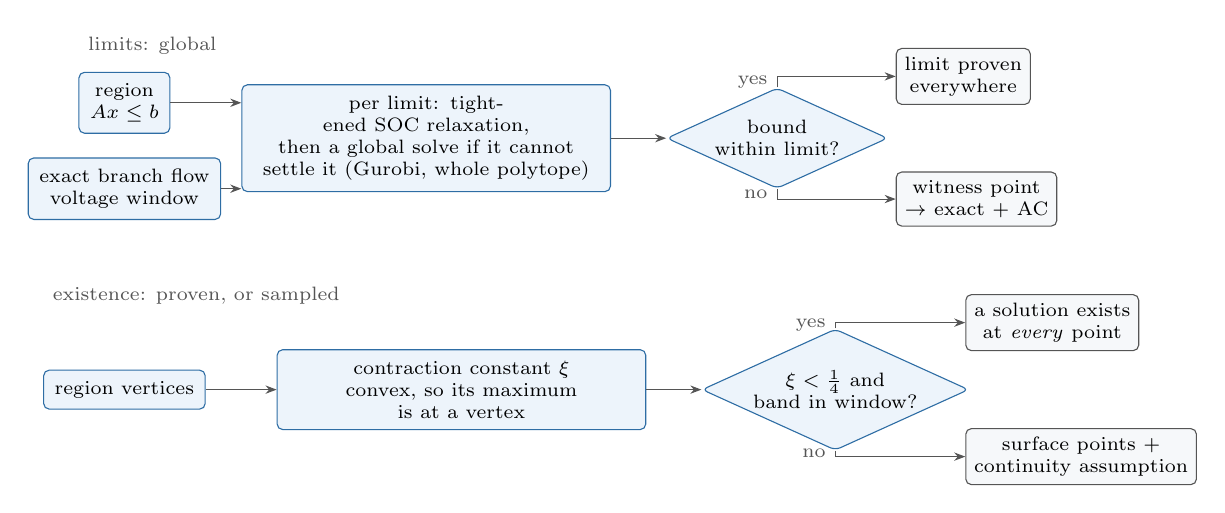
\begin{tikzpicture}[node distance=5mm and 7mm]
\node[blk] (reg) {region\\$Ax \le b$};
\node[blk, below=3mm of reg] (mod) {exact branch flow\\voltage window};
\node[blk, right=9mm of reg, yshift=-4.5mm, text width=4.4cm] (solve)
  {per limit: tightened SOC relaxation,\\then a global solve if it cannot\\settle it (Gurobi, whole polytope)};
\node[blk, diamond, aspect=2.2, inner sep=1pt, right=of solve] (dec) {bound\\within limit?};
\node[res, above right=1mm and 8mm of dec] (ok) {limit proven\\everywhere};
\node[res, below right=1mm and 8mm of dec] (bad) {witness point\\$\rightarrow$ exact + AC};
\draw[arr] (reg.east) -- (solve.west |- reg.east);
\draw[arr] (mod.east) -- (solve.west |- mod.east);
\draw[arr] (solve) -- (dec);
\draw[arr] (dec.north) |- node[lab, pos=0.25, left] {yes} (ok.west);
\draw[arr] (dec.south) |- node[lab, pos=0.25, left] {no} (bad.west);
\node[blk, below=19mm of mod] (vert) {region vertices};
\node[blk, right=9mm of vert, text width=4.4cm] (xi) {contraction constant $\xi$\\convex, so its maximum\\is at a vertex};
\node[blk, diamond, aspect=2.2, inner sep=1pt, right=of xi] (dec2) {$\xi<\frac14$ and\\band in window?};
\node[res, above right=1mm and 8mm of dec2] (ex) {a solution exists\\at \emph{every} point};
\node[res, below right=1mm and 8mm of dec2] (samp) {surface points +\\continuity assumption};
\draw[arr] (vert) -- (xi); \draw[arr] (xi) -- (dec2);
\draw[arr] (dec2.north) |- node[lab, pos=0.25, left] {yes} (ex.west);
\draw[arr] (dec2.south) |- node[lab, pos=0.25, left] {no} (samp.west);
\node[lab, anchor=south west] at ($(reg.north west)+(0,1mm)$) {limits: global};
\node[lab, anchor=south west] at ($(vert.north west)+(0,7mm)$) {existence: proven, or sampled};
\end{tikzpicture}}
\caption{Global limit bounds and solution-existence checks.}
\label{fig:certificate}
\end{figure}

If all bounds lie within their limits, every branch-flow solution in the
voltage window satisfies the selected limits. An attained violation includes a
\emph{witness}: a point of the region together with an exact power-flow
solution that breaches the limit. A loose bound alone is undecided. An unsafe
solution need not make its injection infeasible: another safe root may exist.
The result is \code{limit-violated} unless the all-limits exact solve proves
the witness injection infeasible (\code{witness\_infeasible=True}), in which
case the region is \code{refuted}. The default
\code{confirm\_witnesses=True} performs that exact check; AC is an independent
diagnostic. Existence must be established separately: limit bounds alone do
not show that a solution exists at every injection.

\paragraph{Existence at every point.} With the slack at 1\,p.u., the bus
voltages solve the fixed-point equation
$V = \mathbf 1 - Z\,\bar s \oslash \bar V$, where $Z = Y_{LL}^{-1}$; for a
radial network, $Z_{ij}$ equals the common upstream path impedance of buses
$i$ and $j$. Let $\xi(s) = \max_i \sum_j |Z_{ij}|\,|s_j|$. On the ball
$\max_i|V_i-1|\le\rho$ the map sends the ball into itself when
$\xi \le \rho(1-\rho)$ and contracts with constant $\xi/(1-\rho)^2$; for
$\xi<\frac14$ both hold at $\rho^\ast = (1-\sqrt{1-4\xi})/2$, so by Banach's
theorem a solution exists with every $|V_i-1|\le\rho^\ast$. The injection is
affine in the region coordinates and $|s_j|$ is convex, so $\xi$ is convex over
the region and attains its maximum at a vertex. Checking the vertices
therefore proves existence, inside the band $[1-\rho^\ast, 1+\rho^\ast]$, at every
point. If the band fits the voltage window, the limit bounds apply to that
solution and establish that the region is inner under the stated model: status \code{certified},
scope \code{"inner"} (\code{prove\_existence}; \code{existence="contraction"},
the default). The condition holds on all twelve 4-D \code{9bus} regions of
Table~\ref{tab:certificate}, refuted ones included: $\xi \le 0.154$, a band of
at worst $[0.81, 1.19]$ inside the window $[0.75, 1.25]$. The entries marked
``cert.'' therefore do not depend on the continuity assumption. With the slack at
$v_0$ (\code{slack\_vm\_pu}) the map is $V = v_0\mathbf 1 - Z\,\bar s \oslash \bar V$:
the condition becomes $\xi < v_0^2/4$, the radius
$\rho^\ast = 2\xi/(v_0+\sqrt{v_0^2-4\xi})$ and the band
$[v_0-\rho^\ast, v_0+\rho^\ast]$.

The implementation evaluates the small root as
$\rho^\ast=2\xi/(1+\sqrt{1-4\xi})$ to avoid cancellation at small nonzero
injections. \code{safety} is a finite relative margin in $[0,1)$; zero disables
the additional floating-point margin. An explicit \code{window} is a finite,
strictly increasing positive pair. \code{contraction\_constant} accepts one
point or an $(n,d)$ matrix and returns one value per point. The dense impedance
matrix requires $O(n_{bus}^2)$ work and storage and is assembled from a complete
parent-before-child tree. Supplied topologies must satisfy that ordering.

The interval sweep's tree-sum setup also uses the topological branch order:
it computes depths once and groups only depth/sibling-rank pairs that exist.
Storage for these groups is linear, with at most $O(n\log n)$ sorting work,
so a deep feeder with a wide terminal fan does not scan every empty pair.
This reduces setup work; the contraction condition and the sweep's separate
subtree-incidence storage are unchanged.

\paragraph{Existence by sampling.} The point verifier evaluates uniformly
drawn surface points (Figure~\ref{fig:escalation}); it does not re-sample the
vertices evaluated during construction. When the contraction proof holds,
these samples provide an independent cross-check. Otherwise, as may occur on
heavily loaded or long feeders, they establish existence only at the sampled
points. Extending existence between them requires a continuous high-voltage
solution with no voltage-collapse fold inside the window, giving scope
\code{"conditional\_inner"}. Without a proof or surface existence checks,
the result is \code{limits-certified}.

\paragraph{Subdivision of undecided limits.} A time-out or a numerical failure leaves
a limit \code{undecided}. The worst case over the region is the worst over any
cover of it, so the limit is re-solved on the two halves of the region cut across
its widest coordinate, and so on up to \code{split\_depth} (default 2); the pieces'
bounds combine into a valid bound for the whole region, and smaller pieces give
tighter relaxations. A piece with no solution in the window refutes the region
there, and its witness is retained; it does not mean the entire original
region has no solution. Settled limits are never split;
\code{INF\_OR\_UNBD} stays undecided.

The search window strictly contains the allowed voltage range. It expands
when the usual $[0.5,1.5]$ clipping would remove permitted voltages, so window
infeasibility cannot arise solely from excluding an allowed solution.

\paragraph{SOC screening and bound tightening.}
\label{sec:relax-first}
On a larger network a single global solve
can reach the 60\,s time-out, and a region there has hundreds of limits.
The SOC relaxation ($l v \ge P^2 + Q^2$ instead of $=$) contains every exact
solution, so its optimum also gives a valid bound. A convex solve costs about
10\,ms. Without tightening, it settles only the upper voltage limits. For
$r, x \ge 0$, raising a loss $l_k$ by $\delta$ lowers every voltage below
branch~$k$ by at least $(r_k^2 + x_k^2)\,\delta$. A relaxation free to inflate
losses therefore attains exact losses when maximising a voltage. When it
maximises a current or minimises a voltage, it inflates them up to the window
edge.

Bound tightening restricts these excess losses. Each round bounds every $P_k$ and $Q_k$
from both sides, and every $v_i$ from below, over the current relaxation. It
then adds the cut $v^{lo}_{\mathrm{parent}}\, l_k \le \sec(P_k) + \sec(Q_k)$,
where $\sec$ is the secant of the square on the current bounds
($P^2 \le (a{+}b)P - ab$ on $[a, b]$). Every exact solution satisfies every cut
($l v = P^2 + Q^2$, $v \ge v^{lo}$, and a square lies below its secant). Each
round's relaxation therefore still contains all of them, and so do the bounds
passed on to the global solves.

A limit the relaxation proves is certified with solver status
\code{relaxation}, and its bound is valid but may be looser than the exact
worst case. The remaining limits are solved globally using the tightened
bounds. The first tightening round is unconditional: the initial relaxation
does not settle current or lower-voltage limits, whose global solves may
reach the time limit. Each further round runs while the previous one settled at
least one more limit (\code{relaxation\_rounds}, at most 3 by default;
\code{None} disables the screen). The round count is independent of measured
runtime, so system load does not determine the bounds. A settled limit retains
its relaxation bound. Limits that could determine the reported worst loading,
lowest voltage or highest voltage are then solved globally, in order of worst
bound, until no remaining relaxation
bound is worse than the exact worst case found. The reported worst cases are
therefore exact and reproducible. On the twelve
regions of Table~\ref{tab:certificate} this costs 54\,s instead of 35\,s; \code{stop\_at\_limit=True}
skips the re-solve. \code{workers} solves the remaining limits
in parallel threads, each with its own Gurobi environment.

\begin{center}\small
\begin{tabular}{@{}lrrrr@{}}
\toprule
Region & limits & global only & relax first & by relaxation \\
\midrule
9-bus Method 1 (certified)     & 24  & 2.3\,s & 2.9\,s; 2.1\,s (4 w.)  & 19 \\
9-bus Method 2 (certified)     & 24  & 2.1\,s & 2.0\,s; 1.2\,s (4 w.)  & 19 \\
9-bus Model~I (refuted)        & 24  & 1.9\,s & 1.9\,s; 1.1\,s (4 w.)  & 19 \\
9-bus Method 1, 1p,1q,7p,7q    & 24  & 79\,s  & 3.5\,s                  & 14 \\
\bottomrule
\end{tabular}
\end{center}

\noindent The first three 9-bus entries use axes 2,4,7,0 from
Table~\ref{tab:certificate}; the fourth uses the axis seed. In the fourth,
one $v^{min}$ limit required subdivision after a 60\,s global-solve time-out;
tightening settled it directly. Timed tightening probes gave runtimes of
4\,s or 80\,s, motivating the fixed first round and count-based stopping
rule. The table records earlier measurements with timed further rounds.

Statuses and violations matched the global-only certificate. The largest
bound difference was $1.5\cdot10^{-6}$ in squared per-unit loading, within
solver tolerance. Below 1\,\% loading, this can mean about 1\,\% relative
variation in reported loading. All exact branch-flow extremes lay within the
tightened bounds. A 9-bus global solve cost about four relaxed solves, so
screening offered little benefit unless a time-out was avoided. Tightening proceeds from the slack, with each depth
in parallel: upstream flow bounds restrict downstream losses. Bounding all
flows simultaneously from the initial relaxation settled no additional limits
in the first round.

\begin{table}[h]
\centering\small
\caption{Certificates for 4-D \code{9bus} regions (80-vertex component
budgets, \code{adaptive-ema}, simplex seed, \code{rng} 0).
Entries give globally proven worst-case branch loading and volumes in MW$^4$.
Every limit that could attain the maximum is solved globally.
Refutation witnesses are checked by the exact all-limits model and independent
AC power flow. Reproduce with
\code{python scripts/demo.py conservative -{}-axes 2,4,7,0 -{}-max-vertices 80
-{}-certify}.}
\label{tab:certificate}
\begin{tabular}{@{}llll@{}}
\toprule
Axes & M1, path scope (default) & M1, direct-feeder scope & M2 \\
\midrule
1,3,5,6     & \textbf{cert.} 89.76\% (108) & refuted 100.78\% & \textbf{cert.} 70.59\% (254) \\
2,4,7,0     & \textbf{cert.} 94.11\% (4\,548) & cert. 99.66\% (8\,637) & \textbf{cert.} 92.89\% (3\,767) \\
1p,3q,5p,7p & \textbf{cert.} 98.20\% (2\,429) & refuted 100.93\% & \textbf{cert.} 93.10\% (2\,055) \\
1p,1q,7p,7q & \textbf{cert.} 99.19\% (9\,414) & cert. 99.97\% (14\,769) & \textbf{cert.} 98.81\% (4\,272) \\
\bottomrule
\end{tabular}
\end{table}

\why{The head branch (slack $\to$ bus 7) supplies every lateral and is
transformer-like ($x/r \approx 57$): its reactive loss at rating is
1.56\,Mvar, compared with a 0.026\,MW active loss. On regions without a $Q$
axis, the loss box in Section~\ref{sec:method1} accounts for this reactive loss
and simultaneous losses on other branches. The direct-feeder scope includes
only each POC's feeding branch and omits the head branch's losses from the
shifts, producing the refuted regions in the table. Method~2 tightens branch
limits using loss bounds.}

\code{shrink\_to\_certified} bisects the homothetic contraction factor
$\lambda$ towards the base point and finds the largest passing factor
within the requested tolerance. The conservative builder can apply this
procedure automatically:
\begin{lstlisting}
ConservativeBuilder(method="intersect-shift", certify=True)   # contracts only if refuted
region, cert, lam = orc.shrink_to_certified(region, case, axes)
\end{lstlisting}

\trap{An \code{"inner"} certificate combines global limit bounds with
existence throughout the region under the balanced series-impedance model
with fixed slack voltage. \code{"conditional\_inner"} relies on surface
existence checks and continuity/no-fold between samples;
\code{"limits\_only"} establishes no existence. Comparisons use solver
tolerance (about $10^{-6}$). An \code{undecided} result, including a time-out
unresolved by subdivision, does not certify the region.}

%==============================================================================
\chapter{Compression}
\label{ch:compression}

A grown region often contains vertices with small marginal contributions to
volume. Compression retains fewer vertices while controlling volume loss,
reducing storage and the size of vertex-based optimisation models.

\begin{lstlisting}
small = orc.get_compressor("local-search").compress(
    region, target_vertices=20).polytope

# or to a quality budget instead of a vertex count
result = orc.get_compressor("local-search").compress(
    region, target_vertices=4, max_volume_loss_pct=1.0)
result.volume_loss_pct, result.size_reduction_pct, result.trace
\end{lstlisting}

\begin{center}\small
\begin{tabular}{@{}lp{9.7cm}@{}}
\toprule
\code{local-search} & Greedy: drop the vertex with the smallest marginal volume
  loss. Losses are computed from each vertex's neighbourhood and, after a
  removal, refreshed only for affected neighbours; both calculations are exact
  (Section~\ref{sec:livehull}). \\
\code{star-screened} & Greedy for high dimension: rank vertices by their star
  volume (one pass over the facets), compute exact losses for the
  \code{screen} cheapest (default 4), remove the best. A few hulls per removal,
  independent of the vertex count. \\
\code{hybrid-vns} & Greedy plus backward recycling: every surviving vertex keeps
  a pool of the vertices pruned into it, and variable-neighbourhood search can
  restore a pruned vertex when it improves the retained volume. \\
\code{roulette}   & Randomised greedy over the $k$ cheapest removals. \\
\code{random}     & Uniform removal, used as a baseline. \\
\bottomrule
\end{tabular}
\end{center}

Every compressor returns a polytope contained in its input, using only retained
input vertices.

\paragraph{Threads for independent hulls.} Every marginal loss is its own
Qhull computation, and Qhull releases the interpreter lock. From 5-D up
(\code{PARALLEL\_FROM\_DIM}) \code{LiveHull.marginal\_losses} therefore runs
them in a shared thread pool, with identical results in the same order. On 8
threads the measured speedups were 1.7$\times$ in 5-D, 3.8$\times$ in 6-D and
4.4$\times$ in 8-D; in 3- and 4-D thread overhead exceeded hull cost. An 8-D
compress-and-regrow run went from 26.3\,s to 7.0\,s, with a bit-identical
volume and the same oracle calls. \code{OpenRC.geometry.set\_geometry\_workers(n)}
or \code{OPENRC\_GEOMETRY\_WORKERS} sets the thread count (1 turns threading
off). Pools are keyed by worker count. \code{parallel\_map} completes work in
the calling thread if a pool is closed concurrently; changing the worker
setting releases obsolete pools. A long-lived service or notebook can release
all shared geometry workers with
\code{shutdown\_geometry\_workers()}; the next parallel operation recreates the
pool. The benchmark harness gives each worker process its share of the cores.

All five support live-hull compression through \code{compress\_live}, which
the memory-aware builder uses directly. \code{compress} creates a hull from a
polytope for the duration of the call. Stopping criteria include a vertex
target, cumulative volume-loss budget and hull-memory goal measured after each
removal. A per-removal price limits absolute volume loss. For compressors
implemented through the polytope interface \code{\_run}, the base class passes
the vertices and reloads the live hull afterwards.

\why{In 16-D nearly every pair of vertices shares a facet. \code{local-search}
then refreshes every loss after each removal using full hull evaluations,
requiring 20--80\,s per compression of a 32-vertex region.
\code{star-screened} uses five hulls per removal, and
\code{compressor="auto"} selects it above 6-D.}

\trap{On the tested regions, \code{hybrid-vns} and \code{local-search}
converged to the same final vertex set, although individual recycling steps
increased hypervolume. \code{roulette} improved the extreme-tail results.
Use \code{python scripts/demo.py bench-compress} to compare methods on the
regions of interest. In \code{hybrid-vns}, the second VNS phase searches pruned
points nearest to the first phase's best point, and each recycled point can be
adopted only once.}

%==============================================================================
\chapter{Validation}
\label{ch:validation}

\section{Error and loss rates}

Region quality is estimated by sampling a domain containing the region and
surrounding operating points. Each sample is checked for region membership
and reference feasibility. With $N_R$ the points the region
accepts, $N_D$ the points \emph{proven} feasible, $N_{RD}$ their intersection
and $N_{U,R}$ the unresolved points inside the region:
\begin{align}
\text{error rate} &= 1 - \frac{N_{RD}}{N_R - N_{U,R}}
  &&\text{in-region points that are proven infeasible} \\
\text{loss rate}  &= 1 - \frac{N_{RD}}{N_D}
  &&\text{feasible samples outside the region}
\end{align}

\why{The loss numerator counts feasible points captured by the region,
$N_{RD}$. Substituting $N_R$ can produce a negative loss rate when the region
contains infeasible points. The error-rate denominator excludes unresolved
points because their feasibility has not been established.}

The loss rate is conditional on the sampling domain and distribution, not a
whole-space volume ratio. Independent draws carry Wilson 95\% intervals;
observing zero violations in 200 trials leaves greater uncertainty than in
20\,000 trials. Sobol
sequences, scenarios drawn without replacement and custom samplers that do
not declare independence retain point estimates but return \code{NaN}
interval bounds; a binomial confidence claim would be unjustified.

\begin{lstlisting}
quality = orc.evaluate_region(region, case, axes,
                              reference="acpf", n_samples=1000,
                              n_workers="auto",
                              escalate_to=("socp", "exact"))
print(quality.summary())
quality.error_rate, quality.loss_rate, quality.is_conservative
quality.violating_points, quality.unresolved_points, quality.adjudications
\end{lstlisting}

\section{Samplers}

\begin{center}\small
\begin{tabular}{@{}lp{9.5cm}@{}}
\toprule
\code{uniform-box} & Uniform in the region's bounding box grown by a margin,
  extending the validation domain beyond the region's coordinate bounds. \\
\code{sobol-box}   & Low-discrepancy points for more even coverage at a given
  number of reference solves. \\
\code{in-region}   & Uniform inside the region, for error-rate estimation.
  Rejection sampling falls back to a cone decomposition at its work budget. \\
\code{scenarios}   & Recorded operating points, suitable for validation
  against measured profiles. \\
\code{surface}     & Uniform on the region's boundary (area-weighted facet
  simplices), probing the facets between vertices for the certificate's
  existence checks. \\
\bottomrule
\end{tabular}
\end{center}

Samplers return an $(n,\mathrm{dim})$ matrix, including $(0,\mathrm{dim})$ for
an empty draw. Sobol preserves integer or \code{numpy.random.Generator} seeds.
Explicit boxes use paired finite bounds, and rejection sampling has a fixed
draw budget. Blocked surface sampling uses under 20 MiB of traced temporary
memory on a 65,536-facet 16-D
cross-polytope, versus over 360 MiB unblocked (stored hull and native allocations
excluded). Stable simplex measures and scaled log-area weights retain slender
facets without Gram cancellation or absolute-area overflow.

Scenario inputs are finite snapshots with the region's dimension. A result
with no decided in-region samples is \emph{undecided}. The in-region sampler offers
\code{method="auto"}, \code{"rejection"} and \code{"cones"}. Cones are selected
by volume and sampled with Dirichlet coordinates, avoiding poor box acceptance
in thin regions. The automatic fallback preserves uniformity and matches the
rejection draws wherever rejection succeeds.

\section{Adjudication of unresolved reference verdicts}
\label{sec:adjudication}

\file{OpenRC/validation/adjudicate.py}

\begin{enumerate}
\item AC power flow evaluates the point using several initialisations and algorithms.
\item Any answer without reference evidence is escalated. An outer relaxation
  (\code{socp}) can prove infeasibility but never feasibility; an inner
  approximation can prove feasibility but never infeasibility. The adjudicator
  enforces this from each oracle's declared role.
\item The exact global solve attempts a definitive verdict.
\item A solver timeout or numerical failure stays \code{INCONCLUSIVE}. The point
  is listed and excluded from the error-rate denominator.
\end{enumerate}

\why{Newton--Raphson can fail at a feasible point because of its initial
state or an ill-conditioned Jacobian. Treating such failures as infeasibility
would inflate the estimated modelling error. Rejections outside the region
also require evidence to avoid biasing the loss estimate. A weak reference may
require escalation for every sample; a converged, limit-compliant AC solution
provides a less expensive first-stage witness when its physics matches the target.}

When AC power flow \emph{converged} outside a limit and a compatible escalation
finds a safe alternative solution, the first root did not prove infeasibility.
Such a point is a \emph{singular point}: it counts as feasible and is
reported separately, in \code{RegionQuality.singular\_points} (and
\code{VerificationReport.singular\_points}; \code{n\_singular\_points} counts
them), with a SINGULAR line in the summary. The flag can indicate an alternative
nonlinear root or a tolerance effect, not necessarily a voltage-collapse
singularity. Different slack setpoints, line charging, voltage/current limits
or dispatch models require a separate comparison: an escalation without a
known relation to the reference physics leaves the point unresolved.
ACOPF and fixed-dispatch branch flow have no automatic inclusion relation.
Surface certificates target branch flow explicitly; a different AC model
cannot supply their existence evidence.

\code{PointVerifier(target\_model="primary")} uses the primary's physical
family: a weak linear or DC stage still needs evidence about the underlying
exact branch-flow or AC family. Model-relative quality comparisons use
\code{adjudicate=False}. A custom verifier passed to
\code{certify\_inner\_region} must expose a compatible
\code{reference\_oracle} or explicitly declare
\code{target\_model="branch-flow"}.

With default \code{adjudicate=True}, outer-model feasibility and answers
from individual linear or DC models also need escalation, inside and outside
the region. An absent optional escalation solver leaves points unresolved
and is attempted only once per adjudicator. Construct a new adjudicator to
retry after installing a solver.
An exact branch-flow stage on a meshed or otherwise unsupported network is
recorded as unavailable rather than treated as infeasible. An escalation model
declaring no reference-evidence capability is skipped without solving it.
\code{adjudicate=False} retains model-relative comparisons; in that mode an
outer reference provides only a lower bound on error and unknown model
relationships carry no AC/exact guarantee, as noted in the emitted warnings and
summaries.

\section{Global certification and Monte Carlo verification}
\label{sec:verify}

\file{OpenRC/validation/verify.py}, \file{pointcheck.py}, \file{certify.py}

\code{verify\_inner\_region} provides two modes with different evidential
strength (Figure~\ref{fig:modes}):

\begin{description}
\item[\code{mode="surface"}] The certificate of Section~\ref{sec:certificate}:
  global limit bounds, existence proven at every point where the contraction
  condition holds, and points on the region's surface. Only where the condition
  fails does the inner conclusion use the no-fold assumption. A violating
  solution returns a witness (\code{limit-violated}); an injection proven
  infeasible refutes the region (\code{refuted}).
\item[\code{mode="monte-carlo"}] Uniform draws in a large cube,
  \code{cube\_scale} times the region's widest extent. Only the draws inside
  the region are checked. For slender 4-D regions, fewer than 1\% of draws may
  fall inside. \code{min\_inside} continues sampling to obtain enough interior
  points. A \code{passed} result with a Wilson interval provides statistical
  evidence rather than an inner-region proof.
\end{description}

\begin{figure}[htbp]
\centering
\begin{subfigure}[t]{0.47\textwidth}
\centering
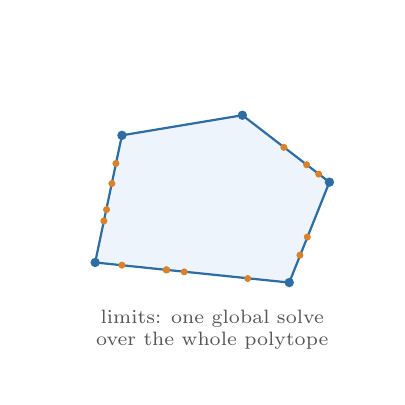
\begin{tikzpicture}[scale=0.85]
\filldraw[fill=notebg, draw=nbblue, thick]
  (-1.60,-0.90) -- (1.30,-1.20) -- (1.90,0.30) -- (0.60,1.30) -- (-1.20,1.00) -- cycle;
\foreach \p in {(-1.20,-0.94),(-0.53,-1.01),(-1.47,-0.28),(1.74,0.42),(1.57,-0.52),
  (-1.43,-0.11),(-0.27,-1.04),(1.22,0.82),(-0.54,-1.01),(-1.35,0.28),(1.46,-0.79),
  (1.56,0.56),(0.68,-1.14),(-1.29,0.58)} \fill[warnrule] \p circle (1.5pt);
\foreach \p in {(-1.60,-0.90),(1.30,-1.20),(1.90,0.30),(0.60,1.30),(-1.20,1.00)}
  \node[vtx] at \p {};
\node[lab, align=center] at (0.15,-1.9) {limits: one global solve\\over the whole polytope};
\draw[white] (-2.6,-2.6) rectangle (2.6,2.6);
\end{tikzpicture}
\caption{\code{surface}: limits proven over the whole polytope; existence
checked at surface points (orange), not at the vertices (blue).}
\end{subfigure}\hfill
\begin{subfigure}[t]{0.47\textwidth}
\centering
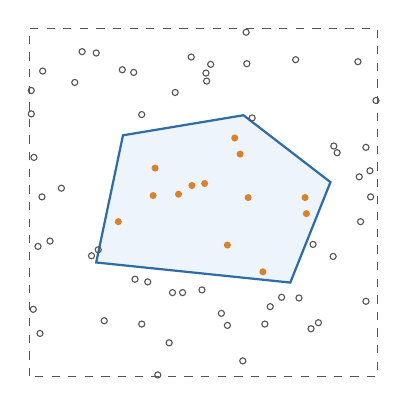
\begin{tikzpicture}[scale=0.85]
\draw[nbgrey, dashed] (-2.6,-2.6) rectangle (2.6,2.6);
\filldraw[fill=notebg, draw=nbblue, thick]
  (-1.60,-0.90) -- (1.30,-1.20) -- (1.90,0.30) -- (0.60,1.30) -- (-1.20,1.00) -- cycle;
\foreach \p in {(1.54,-0.17),(-1.27,-0.29),(0.02,0.28),(0.67,0.07),(-0.72,0.51),
  (0.55,0.72),(0.89,-1.04),(0.36,-0.64),(-0.17,0.25),(-0.37,0.12),(0.47,0.96),
  (-0.75,0.10),(1.52,0.07)} \fill[warnrule] \p circle (1.5pt);
\foreach \p in {(0.65,2.07),(1.43,-1.43),(-1.04,1.94),(-2.57,1.67),(-1.02,-1.15),
  (2.58,1.52),(0.64,2.54),(-1.48,-1.77),(0.59,-2.37),(-2.41,0.08),(-0.18,2.17),
  (-0.02,-1.31),(-2.54,-1.60),(1.00,-1.56),(-0.68,-2.58),(1.72,-1.80),(-1.21,1.98),
  (0.05,1.81),(0.73,1.26),(-2.12,0.21),(0.04,1.93),(-2.29,-0.58),(-0.92,-1.82),
  (1.64,-0.63),(2.49,0.47),(0.92,-1.82),(-0.31,-1.35),(-0.51,-2.10),(2.43,-1.48),
  (1.95,0.84),(-1.92,1.79),(2.31,2.10),(0.36,-1.84),(-1.60,2.23),(0.27,-1.66),
  (2.00,0.74),(-0.46,-1.35),(-2.40,1.96),(-0.92,1.31),(-2.47,-0.66),(-2.44,-1.96),
  (2.43,0.82),(1.94,-0.81),(1.38,2.13),(-1.81,2.25),(-2.57,1.32),(1.61,-1.89),
  (-0.42,1.64),(-2.53,0.67),(1.17,-1.42),(-1.57,-0.71),(-1.67,-0.80),(2.33,0.38),
  (-0.83,-1.19),(2.35,-0.29),(2.50,0.08),(0.11,2.06)}
  \draw[nbgrey] \p circle (1.3pt);
\end{tikzpicture}
\caption{\code{monte-carlo}: uniform draws in a cube; only the 13 of 70 that
land inside (orange) are checked.}
\end{subfigure}
\caption{The two verification modes, in 2-D.}
\label{fig:modes}
\end{figure}

In both modes, \code{PointVerifier} applies the stages in
Figure~\ref{fig:escalation}. A stage can settle a point only when its physical
model and operating limits match the target.

\begin{figure}[htbp]
\centering
\resizebox{\textwidth}{!}{%
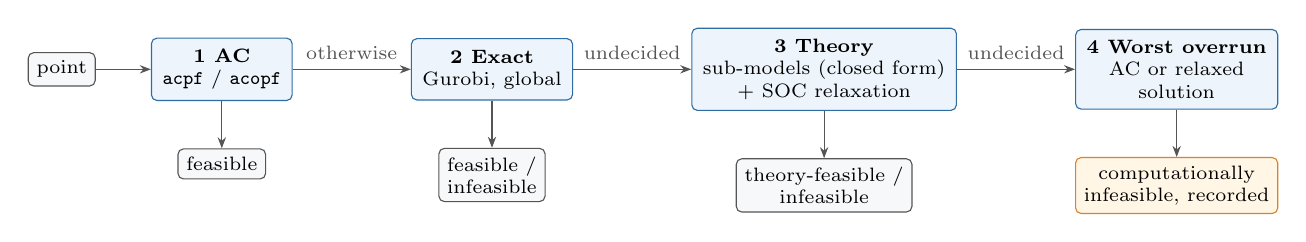
\begin{tikzpicture}[node distance=15mm]
\node[res] (pt) {point};
\node[blk, right=7mm of pt] (ac) {\textbf{1\ AC}\\\texttt{acpf} / \texttt{acopf}};
\node[blk, right=of ac] (ex) {\textbf{2\ Exact}\\Gurobi, global};
\node[blk, right=of ex] (th) {\textbf{3\ Theory}\\sub-models (closed form)\\+ SOC relaxation};
\node[blk, right=of th] (wo) {\textbf{4\ Worst overrun}\\AC or relaxed\\solution};
\draw[arr] (pt) -- (ac);
\draw[arr] (ac) -- node[lab, above] {otherwise} (ex);
\draw[arr] (ex) -- node[lab, above] {undecided} (th);
\draw[arr] (th) -- node[lab, above] {undecided} (wo);
\node[res, below=6mm of ac] (o1) {feasible};
\node[res, below=6mm of ex] (o2) {feasible /\\infeasible};
\node[res, below=6mm of th] (o3) {theory-feasible /\\infeasible};
\node[res, below=6mm of wo, draw=warnrule, fill=warnbg] (o4) {computationally\\infeasible, recorded};
\foreach \a/\b in {ac/o1, ex/o2, th/o3, wo/o4} \draw[arr] (\a) -- (\b);
\end{tikzpicture}}
\caption{Point-verification stages. Each stage uses evidence only in the
direction it proves; a point leaves the chain at the first stage that settles
it.}
\label{fig:escalation}
\end{figure}

\paragraph{Oracle evidence contracts.}
Outer-relaxation acceptance leaves exact feasibility unresolved, as does
inner-approximation rejection. These rules also apply to the primary stage.
Individual linear construction models have no inclusion
guarantee on their own, and a shifted oracle answers a different injection.
DC power flow and DC-OPF likewise do not certify AC voltage feasibility.
Their verdicts cannot settle the unshifted reference problem. The two
conservative methods establish feasibility through joint acceptance under
their construction assumptions.

An extension with an unknown reference relationship sets
\code{supports\_adjudication=False}. A reference oracle sets
\code{certifies\_infeasibility=True} only when every negative verdict is a
global infeasibility certificate. Failed iterations and locally converged
overruns do not meet this requirement.
\code{inner\_approximation=True/False} declares proven inner/outer inclusion;
\code{None} alone is not such a guarantee. \code{describe()} records both
capabilities. An escalation also requires a known physical relationship to the
target; capability flags alone do not establish it. Unknown oracle types
cannot supply cross-model proof.

\begin{enumerate}
\item \textbf{AC} (\code{acpf}, or \code{primary="acopf"}). A converged
  solution within limits: \code{feasible}.
\item \textbf{Exact}, the Gurobi global solve. It proves \code{feasible} or
  \code{infeasible}.
\item \textbf{Theory}: the two sub-models of the region's own method, read
  from its metadata and evaluated in closed form
  (Section~\ref{sec:closed-form}). For Method~1 the point must be accepted
  at every corner of the $P$/$Q$ loss-shift box; when every lossy branch
  feeds a region bus this is the construction's own argument, and
  acceptance is \code{theory-feasible}, as it is for Method~2 with the subtree
  scope (Section~\ref{sec:method2}). Otherwise acceptance is recorded but
  does not settle the point. The SOC
  relaxation also runs; if this outer model has no solution within
  limits, the point is \code{infeasible}. A minimal overrun of at most
  $10^{-4}$ counts only with the solver's infeasibility certificate, because at
  feasible points MOSEK can still return a small positive overrun. The
  relaxation is stated on a power base a decade below the network's load, its voltage band
  always contains the case's limits, and on a meshed network the exact and
  theory stages are reported unavailable instead of aborting the run.
\item \textbf{Worst overrun}. A point unresolved by the preceding stages is recorded
  as computationally infeasible (\code{computationally-infeasible}), together
  with its most severe limit overrun. The overrun comes from the AC solution if the power flow converged
  (lines and transformers against their own loading limits, buses against their own voltage limits),
  and otherwise describes the relaxed primal solution. The minimisation
  solver's proven dual/global lower bound on the common overrun can prove
  infeasibility; its primal objective is an upper bound and cannot do so.
  The displayed element is a diagnostic, not a universal lower bound on that
  element's violation.
\end{enumerate}

\begin{lstlisting}
report = orc.verify_inner_region(region, case, axes, mode="surface")
report = orc.verify_inner_region(region, case, axes, mode="monte-carlo",
                                 n_points=5000, min_inside=200)
report.status, report.records, report.computationally_infeasible
print(report.summary())
\end{lstlisting}

\trap{Monte Carlo did not detect the violations in Tables~\ref{tab:certificate}
and~\ref{tab:audit}: 187--505 in-region points (4-D) and 1\,000 draws (3-D)
were insufficient to detect the small violating subsets. Sampling estimates
rates; an inner-region claim requires global bounds and existence evidence.}

%==============================================================================
\chapter{Applications}
\label{ch:applications}

Representing the feasible set as $Ax \le b$ allows downstream decision problems
to enforce grid constraints without solving a power flow at each evaluation.

\begin{lstlisting}
app = orc.get_application("capacity-allocation")
batch = app.solve_batch(region, loading_ratio_scenarios)
batch.mean_objective, batch.mean_ms, batch.to_frame()
\end{lstlisting}

\begin{description}
\item[\code{storage-sizing}] Minimum weighted correction that moves a congested
  operating point back into the region:
  $\min \sum_i |\hat P_i - P_i|$ s.t.\ $P \in \mathcal{R}$.
\item[\code{capacity-allocation}] Largest weighted orthotope inside the region.
  Each POC receives a capacity range whose joint orthotope must be contained
  in the region.
\end{description}

\why{Capacity allocation expresses the worst of the $2^d$ orthotope corners analytically.
For each facet $a^\top P \le b$ the corresponding constraint is
$a^\top P_{low} + \max(a, 0)^\top(\alpha \odot \Delta P) \le b$, so the LP has
one row per stored halfspace inequality and $O(m \cdot d)$ memory for $m$
rows, compared with $O(m \cdot d \cdot 2^d)$ for corner enumeration. This exact
reformulation agrees with brute-force enumeration to $10^{-15}$.}

Compression reduces the vertex count, but can increase the number of facets
and stored inequalities. Its effect on downstream LP size and runtime must
therefore be measured.

Both applications are linear programs solved through SciPy's HiGHS interface.
Using a common solver supports comparison of the formulations' size and runtime.

%==============================================================================
\chapter{Execution: memory and workers}
\label{ch:execution}

\section{Memory}

\file{OpenRC/resources.py}

Hull memory depends on the facet count, which is not determined by the vertex
count in four or more dimensions. OpenRC provides direct measurements and
budget estimates:

\begin{lstlisting}
from OpenRC.resources import measure_polytope_memory, extrapolate_vertex_budget
measure_polytope_memory(region)                    # actual bytes
extrapolate_vertex_budget([(30, 4399), (60, 28414)], dim=8, limit_mb=500)
\end{lstlisting}

\begin{center}\small
\begin{tabular}{@{}rrrr@{}}
\toprule
$d$ & Vertices & Facets & Hull memory \\
\midrule
3 & 80 & 156 & 0.010\,MiB \\
8 & 40 & 10\,278 & 1.335\,MiB \\
8 & 80 & 53\,205 & 6.906\,MiB \\
\bottomrule
\end{tabular}
\end{center}

During growth, \code{live.memory\_mb()} estimates live-hull storage at
$40d+108$ bytes per facet. Memory-aware schedules use this estimate
(Section~\ref{sec:adaptive}).

\code{MemoryGuard} checks the process budget cooperatively between iterations:

\begin{description}
\item[Already over budget before any work] \code{MemoryBudgetExceeded}
  propagates. There is no partial region to return.
\item[Budget exceeded during growth] The loop stops, the region built so
  far is returned, and \code{stopped\_because} records why.
\end{description}

\why{Polling at iteration boundaries preserves partial results for
\code{MemoryAwareBuilder}. An immediate process exit through
\code{os.\_exit(1)} would discard them. Freed memory is not always returned to
the operating system, so a later round may start above the RSS budget. In that
case the builder stops and returns its best region.}

\section{Workers}
\label{sec:workers}

\file{OpenRC/parallel.py}

Random seeding, axis probes and validation sweeps consist of independent
queries and can run in parallel. The growth loop is sequential: every inserted
vertex changes the next decision.

\begin{lstlisting}
orc.evaluate_region(region, case, axes, n_workers="auto")
ExpansiveBuilder(seed="random", n_workers="auto")
\end{lstlisting}

\begin{description}
\item[Processes by default] A Pyomo model and its solver are stateful and not
  thread-safe. Each process worker reconstructs its own oracle from a registry
  recipe. Thread workers also receive separate oracles. Pyomo's output capture
  and bookkeeping remain process-global, so complete operations share a reentrant
  guard across threads, including the verifier's soft relaxation. Quiet AC
  Iwamoto retries use the same output lock. Use spawned processes for parallel
  Pyomo solves; analytic queries, ordinary AC retries and direct modelling
  layers do not acquire the Pyomo guard.
\item[Deterministic] Seeding and validation return the same results with one
  or eight workers. Before dispatch, the requested case is compared with the
  case reconstructed from its \code{get\_case} recipe, including limits, base
  injections and all network tables; this takes about 1\,ms. A variant derived
  with \code{case.rebuild} or \code{dataclasses.replace} runs serially with a
  warning if the recipe does not reproduce it. Evaluating the original recipe
  for \code{9bus} after raising \code{vm\_min\_pu} to 0.97 would give a region
  of 512.6 rather than 440.3\,MW$^3$.
  In-place physical edits instead fail at the configuration guard and require
  explicit reconstruction before another model can use them.
\item[Automatic worker selection] Spawned-pool startup takes seconds because
  each worker imports \code{pandapower} and reconstructs the case.
  \code{"auto"} times a calibration batch after the initial model build,
  which can otherwise inflate the estimate tenfold. Pool startup is measured
  once per session for each case, oracle and worker count. Parallel execution
  is selected only when the predicted saving exceeds startup cost. Random
  seeding reuses one pool across batches instead of starting a pool per batch.
\end{description}

\begin{figure}[htbp]
\centering
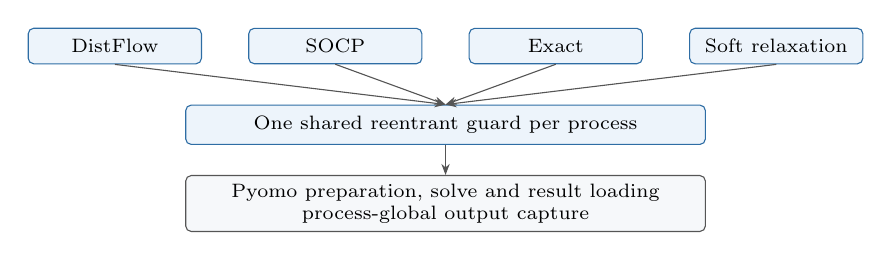
\begin{tikzpicture}
  \node[blk, minimum width=2.2cm] (df) at (0,0) {DistFlow};
  \node[blk, minimum width=2.2cm] (soc) at (2.8,0) {SOCP};
  \node[blk, minimum width=2.2cm] (ex) at (5.6,0) {Exact};
  \node[blk, minimum width=2.2cm] (soft) at (8.4,0) {Soft relaxation};
  \node[blk, minimum width=6.6cm] (guard) at (4.2,-1.0)
    {One shared reentrant guard per process};
  \node[res, minimum width=6.6cm] (capture) at (4.2,-2.0)
    {Pyomo preparation, solve and result loading\\process-global output capture};
  \foreach \item in {df,soc,ex,soft} \draw[arr] (\item.south) -- (guard.north);
  \draw[arr] (guard) -- (capture);
\end{tikzpicture}
\caption{Pyomo operations share a process-level guard for output capture and
  bookkeeping. Quiet Iwamoto redirection uses the same guard; direct layers
  bypass it, and spawned processes have independent guards.}
\label{fig:pyomo-guard}
\end{figure}

A custom Pyomo adapter should guard preparation, solving and result inspection
as one operation:
\begin{lstlisting}
from OpenRC.powerflow.modeling import synchronized_pyomo

@synchronized_pyomo
def query_pyomo(prepare, solve, read_result):
    model = prepare()  # include parameter updates
    result = solve(model)
    return read_result(model, result)
\end{lstlisting}
The guard covers OpenRC and participating extensions. External unguarded
Pyomo calls or output redirection remain outside its scope.
Equation candidates preserve the caller's warning policy across threads:
dense Newton steps do not modify warning filters, while sparse steps protect
their temporary rank-warning policy. A singular Jacobian causes the candidate
to be rejected and is not treated as evidence of model infeasibility.

Under solver-backed Pyomo evaluation, a 9-bus query takes approximately 1\,ms,
so batches of 1\,200 queries complete faster in a single process than in a
spawned worker pool; \code{n\_workers="auto"} selected serial execution in that
measurement.

\trap{Scripts using process workers need an
\code{if \_\_name\_\_ == "\_\_main\_\_":} guard, because \code{spawn} re-imports
the entry module. In a notebook or piped stdin OpenRC detects that spawned
import cannot be used and falls back to threads with an explanation, avoiding
\code{BrokenProcessPool} failures.}

\subsection{Batch and solver lifetimes}

\code{oracle.feasible\_mask(axes, points)} evaluates analytic DistFlow in
bounded blocks of injections, flows, voltages and limits. The general batch
and pool interfaces use this hook. A subclass or instance customisation of
\code{feasible\_at}, \code{is\_feasible}, \code{verdict} or
\code{\_verdict} uses its own single-point path, preserving any additional
constraints. Scalar, thread and spawned-process
evaluation of the same points give the same verdicts, in input order, with the
same call counts.
\code{OracleStats.record\_many} reduces ordinary batch counters in NumPy,
while preserving one event per point for an overridden logging callback.
\code{map\_rays(..., stats=stats)} collects worker query counts,
feasible counts and query time without counting start-up probes.

\begin{lstlisting}
with orc.get_oracle("exact", case, modeling="gurobi") as oracle:
    mask = oracle.feasible_mask(axes, points)
# The persistent direct solver is released, even on an exception.
oracle.close()  # idempotent; later queries may lazily rebuild
\end{lstlisting}

\code{PointVerifier} supports \code{with} and idempotent \code{close()}.
Each multi-stage check, including diagnostics and cleanup, is serialised.
Named stages rebuild lazily after close; caller-supplied primaries remain
open. Inspection of a shared AC oracle holds its query lock through the power
flow and result reading, preserving the correspondence between a point and its
diagnostics.

\code{verify\_inner\_region}, \code{certify\_inner\_region} and
\code{evaluate\_region} release models they construct, including on exceptions;
caller-supplied instances remain open. The reported time for
\code{evaluate\_region} includes cleanup. A directly managed
\code{Adjudicator} supports \code{with} and \code{close()}, and cannot be
queried after close. Escalation recipes are materialised once for execution
and provenance. Cleanup covers Pyomo-native tasks, environments and candidate
resources, including models constructed before a later factory fails.

Sequential \code{FeasibilityPool} instances own distinct oracles and close
them on exit. A worker's recipe cache holds at most four models and closes an
evicted direct model; \code{OpenRC.parallel.clear\_worker\_cache()} explicitly
clears the calling thread's cache. Thread pools reuse these models during
execution and close their owned caches after joining workers, including on
query errors. Cleanup continues through the remaining models if a close fails,
and pool close is idempotent.

Oracle worker recipes copy nested construction options independently. Editing
a caller's \code{solver\_options} dictionary afterwards leaves the local and
worker settings unchanged. Options containing opaque caller-owned handles may
be used locally; when they cannot be copied, the worker helpers report a
serial fallback.

The analytic batch timings apply to DistFlow evaluation; they do not establish
speedups for AC or exact solver queries.

%==============================================================================
\chapter{Common workflows}
\label{ch:recipes}

\section{Task reference}

\begin{description}
\item[List available components] \code{orc.registries()}, or
  \code{python scripts/demo.py list}.
\item[Import a pandapower model]
  \code{orc.case\_from\_pandapower(net, axis\_presets=\{"poc": [...]\})} (bus
  IDs refer to the original network). Alternatively, save it with \code{pp.to\_json} and pass
  \code{-{}-case-file} to any CLI command.
\item[Load a built-in pandapower network]
  \code{orc.get\_case("pp:case33bw")}; \code{orc.list\_pandapower\_networks()}
  lists the catalogue.
\item[Select one feeder]
  \code{orc.list\_feeders(net)}, then \code{case\_from\_pandapower(net,
  feeder=k)}.
\item[Construct and save a region]
\begin{lstlisting}
run = ExpansiveBuilder(policy="adaptive-gradient", seed="random").build(
    case, axes, oracle, max_vertices=200)
run.save("out/my_region")        # CSV vertices + JSON provenance
\end{lstlisting}
\item[Load a saved region] \code{orc.Polytope.load("out/my\_region.csv")}
\item[Construct a conservative candidate]
\begin{lstlisting}
from OpenRC.region.conservative import ConservativeBuilder
region = ConservativeBuilder(method="tight-intersect").build(
    case, axes, max_vertices=200).polytope
\end{lstlisting}
\item[Estimate error and loss rates]
\begin{lstlisting}
print(orc.evaluate_region(region, case, axes, reference="acpf",
                          n_samples=2000, n_workers="auto").summary())
\end{lstlisting}
\item[Compress a region]
\begin{lstlisting}
small = orc.get_compressor("local-search").compress(
    region, max_volume_loss_pct=1.0).polytope
\end{lstlisting}
Fewer vertices need not mean fewer halfspace constraints; measure the resulting
LP row count and runtime for the intended application.
\item[Use an AC power-flow oracle]
  \code{orc.get\_oracle("acpf", case)}.
\item[Select mixed active/reactive axes]
  \code{case.resolve\_axes(["1p", "1q", "3p"])}.
\item[Inspect thermal tightening]
  \code{orc.get\_oracle("tight-voltage", case).binding\_tightening()}.
\item[Identify binding operating limits]
\begin{lstlisting}
from OpenRC.validation import diagnose_violations
diagnose_violations(case, axes, quality.violating_points)
\end{lstlisting}
\item[Certify or contract a region]
\begin{lstlisting}
report = orc.verify_inner_region(region, case, axes)     # the certificate
if report.status != "certified":
    region, cert, lam = orc.shrink_to_certified(region, case, axes)
\end{lstlisting}
\item[Set a memory budget for an 8-D build]
\begin{lstlisting}
MemoryAwareBuilder(max_vertices=150, target_vertices=75, rounds=10).build(
    case, case.resolve_axes("all8"), oracle, memory_limit_mb=4096)
\end{lstlisting}
\end{description}

\section{Reading a result object}

\begin{center}\small
\begin{tabular}{@{}>{\raggedright\arraybackslash}p{3.2cm}>{\raggedright\arraybackslash}p{11.3cm}@{}}
\toprule
\code{RegionResult} & \code{.polytope}, \code{.trace}, \code{.oracle\_stats},
  \code{.builder\_info}, \code{.seconds}, \code{.stopped\_because},
  \code{.summary()}, \code{.to\_frame()}, \code{.save()} \\
\code{CompressionResult} & \code{.polytope}, \code{.volume\_loss\_pct},
  \code{.size\_reduction\_pct}, \code{.trace}, \code{.summary()} \\
\code{RegionQuality} & \code{.error\_rate}, \code{.loss\_rate}, the matching
  \code{\_ci} pairs, \code{.is\_conservative}, \code{.violating\_points},
  \code{.unresolved\_points}, \code{.adjudications}, \code{.summary()} \\
\code{BatchResult} & \code{.mean\_objective}, \code{.mean\_ms},
  \code{.n\_solved}, \code{.to\_frame()} \\
\bottomrule
\end{tabular}
\end{center}

\code{stopped\_because} distinguishes termination by the search criterion
(\code{"facet queue exhausted"}) from termination at a configured budget
(\code{"max\_vertices reached"}).

%==============================================================================
\chapter{Command-line interface}
\label{ch:cli}

\begin{lstlisting}[style=sh]
python scripts/demo.py list                 # every registry
python scripts/demo.py case --case pp:mv_oberrhein --feeder 1   # describe a network
python scripts/demo.py tour                 # guided walkthrough

python scripts/demo.py region --case 9bus --axes 247 \
    --seed random --seed-samples 2000 --seed-batch-size 500 \
    --policy adaptive-gradient --workers auto \
    --max-vertices 120 --max-oracle-calls 20000 \
    --memory-limit-mb 4096 --out out/

python scripts/demo.py conservative --case 9bus --axes 247 --validate 1000
python scripts/demo.py conservative --axes 2,4,7,0 --max-vertices 80 --certify
python scripts/demo.py verify    --axes 2,4,7,0 --region out/<file>.csv  # surface
python scripts/demo.py verify    --axes 2,4,7,0 --region out/<file>.csv \
    --mode monte-carlo --min-inside 200
python scripts/demo.py verify    --axes 2,4,7,0 --region out/<file>.csv --shrink
python scripts/demo.py compress  --region out/<file>.csv --target 15
python scripts/demo.py validate  --case 9bus --axes 247 --region out/<file>.csv
python scripts/demo.py apply     --case 9bus --axes 247 --region out/<file>.csv
python scripts/demo.py memory    --case 9bus-scaled --axes all8 --rounds 4

python scripts/demo.py bench-policy   --case 9bus --axes 247
python scripts/demo.py bench-compress --region out/<file>.csv
\end{lstlisting}

\code{--axes} takes a preset name (\code{247}), explicit buses (\code{1,3,6}) or
mixed axes (\code{1p,1q,3p}).

%==============================================================================
\chapter{Extending OpenRC}
\label{ch:extend}

\section{Registration}

\begin{lstlisting}
from OpenRC.compression.base import COMPRESSORS, CompressionResult, Compressor

@COMPRESSORS.register("my-method", doc="One-line CLI description")
class MyCompressor(Compressor):
    name = "my-method"

    def _run(self, polytope, *, target_vertices, max_volume_loss_pct):
        # Return a CompressionResult; preserve axes and provenance.
        ...
\end{lstlisting}

Registration exposes components through factories, CLI choices, benchmarks
and composed workflows. The same pattern serves every family below;
schedules and screens also accept unregistered instances.

\section{Component interfaces}

\begin{center}\small
\begin{tabular}{@{}lll@{}}
\toprule
Family & Base class / shape & Required member \\
\midrule
Case         & factory $\rightarrow$ \code{GridCase} & -- \\
Oracle       & \code{FeasibilityOracle}   & \code{\_check}, optionally \code{\_verdict} \\
Modelling layer & \code{DirectModel}     & \code{verdict} on a \code{ConicForm} \\
Builder      & \code{RegionBuilder}       & \code{build} \\
Seed         & callable                   & returns \code{SeedResult} \\
Facet policy & \code{FacetPolicy}         & \code{select}, optionally \code{observe} \\
Facet screen & \code{FacetScreen}         & \code{pool}, optionally \code{inherit} \\
Compressor   & \code{Compressor}          & \code{\_run}, or \code{\_run\_live} on a live hull \\
Schedule     & \code{CompressionSchedule} & \code{decide}; optionally \code{at\_cap}, \code{finished} \\
Refiner      & \code{Refiner}             & \code{refine}, never lowering the volume \\
Ray strategy & \code{RayStrategy}         & \code{propose}; optionally \code{observe}, \code{accept} \\
Sampler      & \code{Sampler}             & \code{draw} \\
Application  & \code{Application}         & \code{solve} \\
Benchmark method & callable               & \code{(case, axes, oracle, *,} \\
             &                            & \quad\code{max\_vertices, seed)} $\rightarrow$ result \\
\bottomrule
\end{tabular}
\end{center}

\section{Extension requirements}

\begin{itemize}
\item State units and signs; validate finite values and dimensions at boundaries.
\item Inject deterministic RNGs; isolate solver handles and support serial and
  worker-safe construction. Declare physical case-extension parameters as
  dataclass fields so configuration checks include them. Registry recipes
  include OpenRC modelling markers; direct oracles without recipes run serially.
\item Emit provenance; check invariants against a known numerical case; document
  failure as \code{INCONCLUSIVE}, a budget stop, or an explicit exception.
\end{itemize}

%==============================================================================
\chapter{Benchmarks}
\label{sec:benchmark}

\file{OpenRC/benchmark.py}, \file{scripts/benchmark.py}

Method comparisons use multiple axis selections and random seeds. Builder
trajectories can change by a few percent when a boundary point moves by
$10^{-5}$ (Section~\ref{sec:closed-form}), so single-instance results may not
represent performance across a network.
\begin{itemize}[itemsep=0.1em]
\item \code{random\_instances} draws $d$ of a network's bus quantities per
  seed, so every seed is a different region. A draw with an infeasible base
  point is replaced.
\item A \emph{method} is any callable
  \code{method(case, axes, oracle, *, max\_vertices, seed)} returning a
  region result. \code{BENCHMARK\_METHODS} holds examples, and any function of
  that form can be passed instead.
\item \code{run\_benchmark} runs every method on every instance with the same
  vertex budget per dimension ($N = \lceil k d \rceil$). Exceptions raised by a
  method are recorded in the run table rather than propagated.
\item \code{summarize} reports, per network, dimension and method, the
  geometric-mean volume ratio to a baseline over the \emph{paired} instances,
  with a Student-$t$ interval on the log scale, and the win rate. The win
  rate counts every paired instance (a method that finds no volume loses);
  \code{ratio\_excluded} gives how many of them the mean leaves out.
\end{itemize}
Paired ratios account for the large differences in absolute volume between
instances.

\begin{lstlisting}
from OpenRC.benchmark import random_instances, run_benchmark, summarize
instances = random_instances("9bus", dims=[3, 5, 8], seeds=range(8))
runs = run_benchmark(["expansive", "grow-and-polish", my_method], instances,
                     vertices_per_dim=6)
print(summarize(runs, baseline="expansive"))
\end{lstlisting}

\paragraph{Paired comparison results.} 96 instances (4 networks $\times$
3 dimensions $\times$ 8 seeds, P/Q axes, LinDistFlow) and 8 methods at
6 vertices per dimension. The table gives
paired geometric-mean volume ratios. A \textbf{bold} entry has a 95\,\%
interval that excludes 1.

\begin{center}\footnotesize
\begin{tabular}{@{}lrrrrrr@{}}
\toprule
Network & $d$ & axis/simplex & polish/queue & debt/plain & debt-cone/plain & compress/grow \\
\midrule
9bus & 3 & \textbf{1.48} & \textbf{1.03} & 1.09 & 1.07 & \textbf{1.39} \\
9bus & 5 & \textbf{7.88} & \textbf{1.12} & 1.05 & 1.03 & \textbf{1.43} \\
9bus & 8 & \textbf{258} & \textbf{1.25} & \textbf{1.17} & 1.11 & \textbf{2.00} \\
case33bw & 3 & \textbf{8.75} & \textbf{1.28} & 1.09 & \textbf{1.13} & \textbf{2.02} \\
case33bw & 5 & \textbf{145} & \textbf{2.02} & 1.26 & 1.09 & \textbf{1.48} \\
case33bw & 8 & \textbf{16\,483} & \textbf{3.80} & 1.02 & 1.00 & \textbf{1.21} \\
mv\_oberrhein & 3 & \textbf{2.55} & \textbf{1.26} & 1.17 & \textbf{1.10} & \textbf{2.20} \\
mv\_oberrhein & 5 & \textbf{19.3} & \textbf{1.49} & 1.01 & 1.05 & \textbf{1.51} \\
mv\_oberrhein & 8 & \textbf{102} & \textbf{1.85} & 1.03 & 1.00 & \textbf{1.48} \\
CIGRE MV & 3 & \textbf{4.65} & \textbf{1.24} & \textbf{1.09} & 1.06 & \textbf{1.97} \\
CIGRE MV & 5 & \textbf{67.4} & \textbf{1.34} & 1.05 & 1.07 & \textbf{1.39} \\
CIGRE MV & 8 & \textbf{5\,908} & \textbf{1.82} & 1.04 & 1.03 & \textbf{1.49} \\
\bottomrule
\end{tabular}
\end{center}

\noindent Columns: \code{expansive-axis} over \code{expansive-simplex};
\code{grow-and-polish} over \code{facet-queue} at the same vertex count; the
debt screen (count and cone weighting) over plain \code{compress-regrow};
\code{compress-regrow} over plain \code{expansive}.
\begin{description}[itemsep=0.1em]
\item[Seed] The axis seed produced a larger volume on all 96 instances. The
  ratio increased with dimension, from 1.5--8.8 in 3-D to 100--16\,000 in 8-D.
  These results support the \code{"auto"} threshold of 4-D
  (Section~\ref{sec:seeds}).
\item[Relocation] At a fixed vertex count, polishing increased volume by
  3--280\,\%, with a significant difference in all 12 configurations and
  win rates of 88--100\,\%. It required about four times as many oracle calls.
\item[Debt screening] The screen gave 1--17\,\% on average, and 26\,\% in one
  cell. That is significant in only 2 of 12 cells with count weighting and in
  2 of 12 with cone weighting. No significant reduction was observed. Debt
  screening is therefore optional.
\item[Compression] Grow--compress--regrow produced 1.2--2.2 times the volume of plain
  growth at the same final vertex count, for about 2.5 times the calls and,
  in 8-D, 10--16\,s more per run.
\end{description}
The \code{mv\_oberrhein} rows (\code{pp:mv\_oberrhein}, \code{feeder=1}) come
from a separate run of the same command on a different machine. On one of its
8-D instances (seed 3), Qhull could not insert a vertex during a
\code{compress-regrow} round in any of its fallback modes. Growth stops at the
last valid hull in that case, and the best region so far is returned.

\section{Computational performance across networks}
\label{sec:performance}

\file{scripts/benchmark\_performance.py} measures oracle queries, ray searches,
region builds, geometry and certification on \code{9bus}, \code{pp:case33bw},
\code{pp:mv\_oberrhein} (\code{feeder=1}) and CIGRE MV (load 0.8). Comparisons use the same points, rays or
instances under each setting, with 95\,\% Student-$t$ intervals on the log
scale for ratios. Verdicts, boundaries, volumes and certificate statuses are
also compared.
\begin{lstlisting}
python scripts/benchmark_performance.py                      # all six sections
python scripts/benchmark_performance.py --sections oracle rays --out perf.json
\end{lstlisting}
The numbers below are from one run on a 10-core Apple-silicon machine
(Python~3.13, Gurobi, MOSEK, pandapower). The \code{pp:mv\_oberrhein} ratios
(ray searches and AC builds) were measured separately on a 2-core x86 machine
without Gurobi or MOSEK; its solver-backed and multi-thread measurements are
not included.

\paragraph{Oracle queries.} Sixty points per network, at 0.2--1.4 times the
LinDistFlow boundary along random rays over four random axes (a mix of feasible
and infeasible points, as a builder sees them), three passes. Every
configuration agreed with the other implementations of the same model; all four
exact configurations agreed on all 180 points.

\begin{center}\footnotesize
\begin{tabular}{@{}llrrr@{}}
\toprule
Model & configuration & \code{9bus} & \code{case33bw} & CIGRE MV \\
\midrule
LinDistFlow & analytic (default)          & 0.022 & 0.023 & 0.022 \\
            & solver, Pyomo + MOSEK       & 0.80  & 1.79  & 1.27  \\
            & solver, MOSEK Fusion        & 0.084 & 0.100 & 0.106 \\
            & solver, gurobipy            & 0.038 & 0.067 & 0.044 \\
\addlinespace
SOCP        & Pyomo + MOSEK (default)     & 1.18  & 3.35  & 1.96  \\
            & MOSEK Fusion                & 0.43  & 1.19  & 0.75  \\
            & gurobipy                    & 0.20  & 0.95  & 0.45  \\
            & gurobipy + sweep            & 0.42  & 1.02  & 0.64  \\
\addlinespace
exact       & Pyomo + Gurobi (default)    & 2.26  & 25.6  & 3.16  \\
            & gurobipy                    & 0.77  & 35.0  & 0.98  \\
            & gurobipy + sweep, float     & 0.12  & 9.41  & 0.20  \\
            & gurobipy + sweep, interval  & 0.36  & 9.61  & 0.39  \\
\addlinespace
AC          & fresh model                 & 4.17  & 5.26  & 4.78  \\
            & recycled model (default)    & 4.46  & 6.15  & 4.47  \\
\bottomrule
\end{tabular}
\end{center}

\noindent Mean milliseconds per query. The main observations are:
\begin{itemize}[itemsep=0.1em]
\item Closed-form LinDistFlow evaluates a query in 20--30\,$\mu$s across all
  tested networks; solver-backed evaluation is 1.7--78 times slower (slowest
  through Pyomo).
\item The direct layers are 2.6--29 times faster than Pyomo for LinDistFlow and
  SOCP, with the largest gains from gurobipy. For the exact model, global
  optimisation dominates runtime. On \code{case33bw},
  gurobipy was 1.4 times slower (median 2 times), reflecting sensitivity of
  spatial branch-and-bound to an equivalent formulation of the
  model. Keeping presolve's dual reductions there improved the median 2.4-fold
  but made CIGRE MV 19\,\% slower, so it was not adopted.
\item With the sweep, the exact oracle is 2.1--3.6 times faster than through
  gurobipy alone. The mean on
  \code{case33bw} is dominated by its infeasible points, which the sweep never
  decides (median 0.78\,ms). The interval proof adds about 0.2\,ms per query
  over the floating-point test.
\item For SOCP the sweep did not reduce runtime on these networks: it costs
  more than the 0.2--1\,ms conic solve it replaces.
\item Recycling the AC model provided no consistent speed-up across the
  scattered-query benchmarks. When a warm
  start fails, the query needs a second, flat solve.
\end{itemize}

\paragraph{Builds and geometry.}
\begin{center}\footnotesize
\begin{tabular}{@{}lrrrr@{}}
\toprule
Measurement & \code{9bus} & \code{case33bw} & \code{mv\_oberrhein} & CIGRE MV \\
\midrule
AC build, 3-D: bisection $\to$ defaults           & 1.76 & 1.79 & 1.66 & 1.88 \\
\quad of which margin search                      & 1.86 & 1.93 & 1.82 & 1.88 \\
\quad of which recycling                          & 0.95 & 0.93 & 0.91 & 1.00 \\
8-D compress-regrow, 1 $\to$ 8 geometry threads   & 3.49 & --   & --   & --   \\
8-D grow-and-polish, \code{batch} 1 $\to$ 8       & 2.54 & --   & --   & --   \\
\bottomrule
\end{tabular}
\end{center}

\noindent Speed-ups, geometric means over three instances. The AC builds use
the \code{generation} policy at 18 vertices. Their volumes changed by at most
0.021\,\%, and the oracle calls fell from 370--402 to 207--221 per build
(\code{case33bw}: 359 to 191). Threads left volumes and oracle calls
bit-identical. Batching moved volumes by $-1.2$ to $+4.2\,\%$ at the same
oracle calls.

\paragraph{The certificate.} The benchmark certifies the LinDistFlow (Model-I)
region over four random axes at 40 vertices. These candidates generally contain
violations, so the benchmark exercises both limit bounding and global
confirmation of violating witness injections.
\begin{center}\footnotesize
\begin{tabular}{@{}lrrrrr@{}}
\toprule
Network & limits & violated & 1 worker & 8 workers & global only \\
\midrule
\code{9bus}     & 24  & 4  & 2.0\,s   & 0.5\,s  & 1.4\,s \\
CIGRE MV        & 42  & 13 & 3.1\,s   & 0.9\,s  & --     \\
\bottomrule
\end{tabular}
\end{center}
\noindent Statuses were identical in every setting. With 8 workers the
certificate was 3.4--4.0 times faster. Solving every
limit globally is practical only on the 9-bus network. On the larger ones,
single global solves reach the 60\,s time-out.

%==============================================================================
\chapter{Reproducing the archived results}
\label{ch:evidence}

With the settings of the original studies (\code{policy="volume-gain"},
\code{refresh\_gains=False}, a bisection tolerance of $10^{-5}$, 14 generated
points), OpenRC regenerates the archived region with the relative volume
differences reported below.

\begin{table}[h]
\centering\small
\caption{Volume of the archived 14-generated-point region, and OpenRC's
relative difference under each backend. 9-bus: axes \code{247}, Model-I
(\code{lindistflow}).}
\begin{tabular}{@{}lrrr@{}}
\toprule
Comparison & Archived (MW$^3$) & \code{backend="solver"} & \code{"analytic"} (default) \\
\midrule
9-bus Method-I  & 301.000642981 & $+11.1$\,ppm & $+31.4$\,ppm \\
\bottomrule
\end{tabular}
\end{table}

The archive was computed with a conic solver, which rejects feasible points up
to $3.2\cdot10^{-5}$ inside the boundary (Section~\ref{sec:closed-form}). The
exact evaluation has no such band, so its 9-bus region is slightly larger.

For the 9-bus run the maximum directed nearest-vertex difference is
$1.57 \times 10^{-4}$\,MW, consistent with the boundary-search tolerance.

%==============================================================================
\chapter{Notes and limitations}
\label{ch:gotchas}

\section{Changes from the original implementations}
\label{sec:unitbug}

The following issues motivated changes to units, topology handling and
numerical routines:

\begin{description}
\item[Unit conversion] The original scripts were not consistent in their
  units: some converted injections to watts before calling an SI-formulated
  solver, others passed megawatts to the same solver. OpenRC uses MW, Mvar, kV
  and kA at every public interface and converts to SI in one module.
\item[Hard-coded topology] \code{if father == 8} versus \code{if father == 0},
  and \code{v2[son+1]} versus \code{v2[son]} encoded network-specific root and
  variable indices. \code{RadialTopology} now supplies these mappings.
\item[Solver status versus termination condition] Feasibility was read from the
  solver \emph{status}, which reports many infeasible conic programs as
  \code{ok}.
\item[Facet planes] Matrix inversion is singular for a facet plane through the
  origin. OpenRC obtains the planes from Qhull.
\item[A radiality check that counted only lines] Transformers and impedances
  were omitted. OpenRC includes all branch tables, excludes out-of-service rows
  and checks connectivity before root selection (Section~\ref{sec:radiality}).
\item[Ray truncation] A fixed upper bracket could clip a region. An unresolved
  upper bracket now raises \code{UnboundedRayError}.
\item[Placeholder thermal ratings] MATPOWER-derived cases encode absent thermal
  limits as $9900$\,MVA or $99\,999$\,kA. Treating these placeholders as
  physical ratings caused the loss-bounded models and SOCP relaxation to
  disagree with AC power flow on \code{case33bw}. OpenRC detects ratings at or
  above 9\,GVA and treats those branches as unrated
  (Section~\ref{sec:unrated}).
\item[Phase imbalance omitted] The adapter converts asymmetric loads and
  generators to three-phase totals for consistent balanced models.
\item[Switch states ignored] An open ring read as a mesh, and closed bus--bus
  switches read as disconnections. The adapter applies them first.
\item[\code{numpy.longdouble}] The original bisection stored long-double ratios,
  which current \code{numpy.linalg.det} rejects. OpenRC standardises on finite
  \code{float64}.
\end{description}

\section{Practical considerations}

\begin{itemize}
\item \textbf{Bus numbering.} Indices are 0-based and preset names retain the
  paper's 1-based labels. Preset
  \code{"247"} is buses \code{[1,3,6]}.
\item \textbf{Base-point feasibility.}
  A network whose recorded operating point violates its own limits raises
  \code{InfeasibleOriginError} at the origin. On
  \code{pp:create\_cigre\_network\_mv} with \code{load\_scale=1.0}, for
  example, collapsed branch \code{trafo:0} reaches 101.4\% loading; passing
  \code{load\_scale=0.8} restores a feasible base point (80.0\% maximum
  loading, 0.949\,p.u.\ minimum voltage; Section~\ref{sec:loadscale}).
\item \textbf{Scaled ratings.} \code{9bus} and \code{9bus-scaled} use different
  line ratings and lengths.
  Method~2 rejects the default seed origin on \code{9bus-scaled}; this does not
  imply that its feasible set is empty.
\item \textbf{Unrated lines.} MATPOWER-derived cases usually lack physical
  thermal ratings. Branch-flow models may omit placeholder limits; native
  AC/DC/OPF retain the imported ratings. Model-II and Method~2 require an
  explicit rating, for example through \code{default\_rating\_ka}.
\item \textbf{Loss shifts on deep feeders.} The Method~1 path-scope shift can
  exceed the width of a component region. Failure to find a slice centre does
  not establish emptiness; inspect the reported shift and search result.
\item \textbf{Worker overhead.} Process start-up can make small runs slower.
  Use \code{n\_workers="auto"} to account for this cost.
\item \textbf{Compressor selection.} \code{hybrid-vns} did not consistently
  outperform \code{local-search} in the reported benchmarks.
\item \textbf{Memory budgets.} A fixed vertex count does not bound hull memory.
  In 8-D the published
  $78\to58$ rule achieves 44\,\% less volume than plain growth within the same
  memory; in 16-D it increases volume only by exceeding the memory budget by
  $5.4\times$. Pass an explicit memory limit to \code{"adaptive"} (or
  \code{max\_hull\_mb} to \code{ray-growth}).
\item \textbf{High-dimensional seeds.}
  \code{seed="auto"} is \code{axis} from 4-D up; forcing \code{simplex} there
  reduced volume by factors ranging from a few times to several orders of
  magnitude in the reported comparisons.
\item \textbf{Transformer phase shifts.} On a radial network, a phase shift
  rotates every downstream voltage and current by the same angle,
  which changes no magnitude, current or loss. On a meshed network it drives loop
  flows the collapsed line cannot reproduce; the adapter warns either way.
\end{itemize}

\clearpage
\section{Limits of the guarantees}
\label{sec:limits-guarantees}

Table~\ref{tab:certificate} reports certified regions for Method~2 and for
Method~1 with the default path scope. The direct-feeder scope of Method~1 is
refuted on two of four configurations. Method~1 with every lossy branch
feeding a region bus (\code{method1\_covers\_losses}), and Method~2 with the
subtree scope (\code{method2\_covers\_losses}), are labelled theorem-backed.
The \code{certify=True} option attempts certification and contracts a candidate
when necessary. It raises an error if no contraction can be certified within
the configured search budget. When the contraction existence condition holds, the result is
independent of a continuity assumption. All guarantees remain specific to the
selected model, projection assumptions, data and solver tolerances.

By default, the branch-flow formulations (the DistFlow family, SOCP,
\code{exact}, the radial sweep and the inner-region certificate) fix the infeed
voltage at 1.0~p.u.\ and omit line shunt capacitance, whereas the AC/DC oracles
use \code{ext\_grid.vm\_pu} and the full $\pi$-line model.
These modelling differences can substantially shift the feasible boundary: on
CIGRE MV (\code{vm\_pu} $= 1.03$~p.u.), exact branch-flow and AC ray boundaries
differ by up to 52\,\%, compared with 0.02\,\% when the infeed is fixed at
1.0~p.u.\ without charging. Setting \code{slack\_vm\_pu} (to a numerical value,
or \code{"setpoint"} during import) aligns the branch-flow slack voltage with
the AC setpoint. The \code{line\_charging="constant"} option adds each line's pi-model
capacitance, half at each end, as constant reactive sources
$\omega C V^2 / 2$ at the slack voltage (\code{case.charging\_q\_mvar}). With
both, exact and AC ray boundaries on half-loaded CIGRE MV differ by a median
0.05\,\% (largest 0.40\,\%). Constant charging remains an approximation
to the native voltage-dependent shunt model. The defaults (1.0~p.u., charging
omitted) reproduce the published branch-flow models.

\begin{warnbox}
For control or connection decisions, retain the model provenance, resolve
undecided points and validate the saved region against the intended network
model and operating conditions.
\end{warnbox}

%==============================================================================
\chapter{Provenance}
\label{ch:provenance}

The following table links the source studies to their OpenRC modules.
Archived numerical comparisons are given in Chapter~\ref{ch:evidence}.

\begin{center}\small
\begin{tabular}{@{}p{5.1cm}p{9.4cm}@{}}
\toprule
Study or method & OpenRC modules \\
\midrule
Multidimensional hosting-capacity region; Method~1 intersect-and-shift; the
$P_{RD}$ / $P_R$ validation
  & \pymod{region.expansive}, \pymod{region.conservative}
    (\code{intersect-shift}), \pymod{validation.quality} \\[2pt]
Rapid feasibility assessment with two conservative convex models
  & \pymod{powerflow.distflow} (\code{tight-voltage}, \code{tight-flow}),
    \pymod{region.conservative} (\code{tight-intersect}) \\[2pt]
Adaptive facet selection
  & \pymod{region.facet\_policy} (four single-measure policies and three bandit policies) \\[2pt]
Random acceleration by feasible sample clouds
  & \pymod{region.base}, \code{seed="random"} with bounded batching \\[2pt]
Security-region compression by hybrid vertex pruning; memory-efficient
high-dimensional computation
  & \pymod{compression}, \pymod{region.memory\_aware} \\[2pt]
Geometric-programming capacity allocation
  & \pymod{applications} \\
\bottomrule
\end{tabular}
\end{center}

%==============================================================================
\appendix
\chapter{API quick reference}
\label{app:api}

\section{Top level}

\begin{lstlisting}
import OpenRC as orc

orc.registries()                     # everything registered, by family
orc.get_case(name)                   # -> GridCase
orc.get_oracle(name, case, **kw)     # -> FeasibilityOracle
orc.get_builder(name, **kw)          # -> RegionBuilder
orc.get_compressor(name, **kw)       # -> Compressor
orc.get_sampler(name, **kw)          # -> Sampler
orc.get_application(name, **kw)      # -> Application
orc.get_facet_policy(name, **kw)     # -> FacetPolicy
orc.get_schedule(name, **kw)         # -> CompressionSchedule
orc.get_refiner(name, **kw)          # -> Refiner
orc.get_ray_strategy(name, **kw)     # -> RayStrategy
orc.evaluate_region(region, case, axes, ...)   # -> RegionQuality
orc.verify_inner_region(region, case, axes, mode="surface"|"monte-carlo")
orc.certify_inner_region(region, case, axes)   # -> InnerCertificate
orc.shrink_to_certified(region, case, axes)    # -> (region, certificate, lam)
orc.prove_existence(region, case, axes)        # -> ExistenceProof (contraction)

from OpenRC.geometry.live_hull import LiveHull # gain / add / marginal_loss / remove

orc.case_from_pandapower(net, **options)       # any pandapowerNet -> GridCase
orc.list_pandapower_networks()                 # the built-in library
orc.classify_pandapower_networks(names=None)   # which oracles apply (builds them)
orc.list_feeders(net)                          # independently fed parts
orc.Polytope, orc.Verdict, orc.configure_logging
\end{lstlisting}

\section{Registered names}

\begin{center}\small
\begin{tabular}{@{}>{\raggedright\arraybackslash}p{2.6cm}>{\raggedright\arraybackslash}p{11.9cm}@{}}
\toprule
Cases & \code{9bus}, \code{9bus-scaled}, \code{cigre-hv},
  and \code{pp:<name>} for each of the 60 networks in
  \code{pandapower.networks} (including \code{pp:case33bw},
  \code{pp:mv\_oberrhein}, \code{pp:create\_cigre\_network\_mv},
  \code{pp:case9}) \\
Oracles & \code{lindistflow}, \code{lindistflow-vdrop}, \code{tight-voltage},
  \code{tight-flow}, \code{socp}, \code{exact}, \code{acpf}, \code{dcpf},
  \code{dcopf}, \code{acopf} (+ \code{legacy-*} reproduction variants) \\
Builders & \code{expansive}, \code{ray-growth}, \code{conservative}, \code{memory-aware} \\
Seeds & \code{simplex}, \code{axis}, \code{random} \\
Facet policies & \code{volume-gain}, \code{facet-area}, \code{cone-volume},
  \code{generation}, \code{random}, \code{adaptive-ema},
  \code{adaptive-egreedy}, \code{adaptive-gradient} \\
Facet screens & \code{debt} \\
Compressors & \code{local-search}, \code{star-screened}, \code{hybrid-vns},
  \code{roulette}, \code{random} \\
Schedules & \code{vertex-budget}, \code{memory-budget}, \code{adaptive} \\
Refiners & \code{relocation} \\
Ray strategies & \code{facet-queue}, \code{facet}, \code{gradient}, \code{relocation},
  \code{grow-and-polish} \\
Samplers & \code{uniform-box}, \code{sobol-box}, \code{in-region},
  \code{surface}, \code{scenarios} \\
Applications & \code{capacity-allocation}, \code{storage-sizing} \\
\bottomrule
\end{tabular}
\end{center}

\section{Exceptions}

\begin{center}\small
\begin{tabular}{@{}>{\raggedright\arraybackslash}p{4.8cm}>{\raggedright\arraybackslash}p{9.7cm}@{}}
\toprule
\code{MeshedNetworkError} & The network is meshed, disconnected, or contains
  elements outside the DistFlow formulation. Use \code{acpf}, \code{dcpf},
  \code{dcopf} or \code{acopf}. \\
\code{AmbiguousSlackError} & The infeed bus could not be inferred; declare an
  external grid or pass \code{slack\_bus\_override}. \\
\code{InfeasibleOriginError} & The selected origin was rejected or left
  undecided; pass a known feasible origin. Does not imply that the feasible set
  is empty. Solver exceptions are recorded in the \code{OpenRC} log. \\
\code{UnboundedRayError} & A ray could not be bracketed within
  \code{max\_ratio}. \\
\code{EmptyComponentRegionError} & One of a conservative method's two component
  regions could not be built with positive volume; inspect its cause/subclass. \\
\code{InfeasibleComponent\allowbreak{}OriginError} & A component rejects the
  selected start, without proving the component's feasible set empty. \\
\code{EmptyIntersectionError} & Two polytopes do not overlap in a
  full-dimensional way. \\
\code{GeometryNumericsError} & Numerical centring or vertex enumeration failed
  to converge; does not imply that the region is empty. \\
\code{NotOpfReadyError} & Required OPF cost or limit data are missing. \\
\code{UnratedBranchError} & The chosen model bounds losses by thermal ratings
  that some lines do not have. Pass \code{default\_rating\_ka}. \\
\code{MemoryBudgetExceeded} & A configured RSS or modelled hull-memory budget
  has been exceeded. \\
\bottomrule
\end{tabular}
\end{center}

\end{document}
